\hyphenation{Colli-sions}
\hyphenation{Single}
%______________________ Analysis ______________________
\chapter{Search for production of a Higgs boson and a single top quark in multilepton final states in pp collisions at $\sqrt{s}=13$ TeV}\label{ch:analysis}

%______________________ INTRODUCCION ______________________
\section{Introduction}
\label{secc:Intro_analysis}

The Higgs boson discovery, supported on experimental observations and theoretical predictions made about the SM, gives the clue of the way in that elementary particles acquire mass through the Higgs mechanism; therefore, knowing the Higgs mass, the Higgs-boson and Higgs-fermions couplings can be tested. In order to test the Higgs-top coupling, several measurements have been performed, as stated in the chapter \ref{ch:theory}, but they are limited to measure the square of the coupling; however, the production of a Higgs boson in association with a single top quark (\tH) not only offers access to the sign of the coupling, but also, to the CP phase of the Higgs couplings.

This chapter presents the search for the associated production of a Higgs boson and a single top quark events, focusing on leptonic signatures provided by the Higgs decay modes to $\WW$, $\ZZ$, and $\tautau$; the 13 TeV dataset produced in 2016, which corresponds to an integrated luminosity of 35.9\fbinv, is used. It expands previous analyses performed at 8 TeV~\cite{Khachatryan_2015,CMS_AN_2014-140} and searches for associated production of \ttbar pair and a Higgs boson in a multilepton final state channel ~\cite{CMS_AN_2016-211}; it also complements searches in other decay channels targeting $H\to b\bar{b}$~\cite{CMS_PAS_HIG_16-019}.

As shown in section \ref{sec:thq}, the SM cross section of the associated production of a Higgs boson and a single top quark (\tHq) process is driven by a destructive interference between two contributions (see Figure \ref{fig:th_prod}), where the Higgs couples to either the W boson or the top quark; however, if the sign of the Higgs-top coupling is flipped with respect to the SM prediction a large enhancement of the cross section occurs, making this analysis sensitive to such a deviation. A second process, where the Higgs boson and top quark are accompanied by a W boson (\tHW) has similar behavior, albeit with a weaker interference pattern, therefore, a combination of both processes would increase the sensitivity; in this analysis both contributions are combined and referred as  \tH channel. The purpose of this analysis is to investigate the exclusion of the presence of the \tH process under the assumption of the anomalous Higgs-top coupling modifier ($\kappa_t$=-1). The analysis exploits signatures with three leptons in the final state.

The first section present a characteristic \tHq signature as well as the expected backgrounds. The MC samples, data sets, and the physics object definitions are then defined. Following are the background predictions, the signal extraction, and the statistical treatment of the selected events as well as the systematic uncertainties. The final section present the results for the exclusion limits.  



















. Multivariate techniques are used to

discriminate the signal from the dominant backgrounds. The analysis yields a 95%

confidence level (C.L.) upper limit on the combined tH + ttH production cross section

times branching ratio of 0.64 pb, with an expected limit of 0.32 pb, for a scenario with

kt = −1.0 and kV = 1.0. Values of kt outside the range of −1.25 to +1.60 are excluded

at 95% C.L., assuming kV = 1.0.








Dont forget to mention previous constrains to ct check reference \ref{biswas} and references

https://link.springer.com/content/pdf/10.1007%2FJHEP01%282013%29088.pdf (paragraph after eq 2)






















\begin{figure}[!htb]
\begin{center}
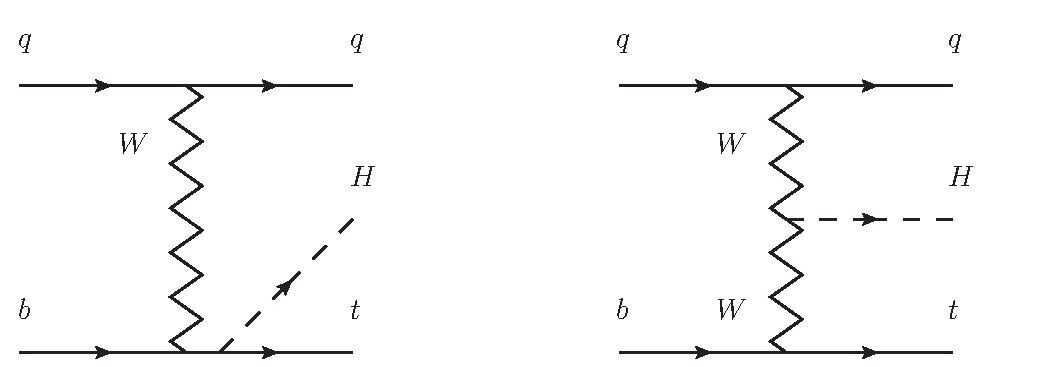
\includegraphics[width=\textwidth]{qtH.pdf}
\end{center}
\caption[The two leading-order diagrams of \tHq production.]{The two leading-order diagrams of \tHq production.}
\label{fig:thq_prod}
\end{figure}

\noindent We selects events with three leptons and a \bjet tagged jet in the final state. The \tHq \ signal contribution is then determined in a fit of the observed data to two multivariate classifier outputs, each trained to discriminate against one of the two dominant backgrounds of events with non-prompt leptons from \ttbar\ and of associated production of \ttbar and vector bosons (\ttW, \ttZ). The fit result is then used to set an upper limit on the combined \ttH, \tHq and \tHW production cross section, as a function of the relative coupling strengths of Higgs and top quark and Higgs and W boson, respectively.

%______________________ Samples  ______________________
\section{Data and MC Samples}
\label{secc:samples}

The data considered in this analysis were collected by the CMS experiment during 2016 and correspond to a total integrated luminosity of 35.9\fbinv. Only periods when the CMS magnet was on were considered when selecting the data samples, that corresponds to the 23 Sep 2016 (Run B to G) and PromptReco (Run H) versions of the datasets. The MC samples used in this analysis correspond to the RunIISummer16MiniAODv2 campaign produced with CMSSW 80X. The two signal samples (for \tHq\ and \tHW) were produced with \textsc{MG5\_}a\textsc{MC@NLO} (version 5.222), in leading-order order mode, and are normalized to next-to-leading-order cross sections, see Tab.~\ref{tab:sigsamples}.Each sample is generated with a set of event weights corresponding to different values of \Ct and \CV couplings as shown in Tab.~\ref{tab:reweight}.

\subsection{Full 2016 dataset and MC samples}
\begin{table}[ht!]
\centering \small
\begin{tabular}{lll}
Sample & $\sigma$ [pb] & BF \\ \hline
\verb|/THQ_Hincl_13TeV-madgraph-pythia8_TuneCUETP8M1/| & 0.7927 & 0.324 \\
\verb|/THW_Hincl_13TeV-madgraph-pythia8_TuneCUETP8M1/| & 0.1472 & 1.0   \\\hline
\end{tabular}
\caption[Signal samples and their cross section and branching fraction.]{Signal samples and their cross section and branching fraction used in this analysis. See Ref.~\cite{THQProdTwiki} for more details.}\label{tab:sigsamples}
\end{table}


\begin{table}[!htbp]
  \centering
  \scriptsize
  \begin{tabular}{lllllll}
        &       & \multicolumn{2}{c}{\tHq} & \multicolumn{2}{c}{\tHW} & \\\hline
   \CV\ & \Ct\  & sum of    & cross         & sum of    & cross        & \\
        &       & weights   & section [pb]  & weights   & section [pb] & LHE weights       \\\hline
   1.0  & -3.0  & 35.700022 & 2.991         & 11.030445 & 0.6409       & LHEweight\_wgt[446]\\
   1.0  & -2.0  & 20.124298 & 1.706         & 5.967205  & 0.3458       & LHEweight\_wgt[447]\\
   1.0  & -1.5  & 14.043198 & 1.205         & 4.029093  & 0.2353       & LHEweight\_wgt[448]\\
   1.0  & -1.25 & 11.429338 & 0.9869        & 3.208415  & 0.1876       & LHEweight\_wgt[449]\\
   1.0  & -1.0  &           & 0.7927        &           & 0.1472       & \\
   1.0  & -0.75 & 7.054998  & 0.6212        & 1.863811  & 0.1102       & LHEweight\_wgt[450]\\
   1.0  & -0.5  & 5.294518  & 0.4723        & 1.339886  & 0.07979      & LHEweight\_wgt[451]\\
   1.0  & -0.25 & 3.818499  & 0.3505        & 0.914880  & 0.05518      & LHEweight\_wgt[452]\\
   1.0  & 0.0   & 2.627360  & 0.2482        & 0.588902  & 0.03881      & LHEweight\_wgt[453]\\
   1.0  & 0.25  & 1.719841  & 0.1694        & 0.361621  & 0.02226      & LHEweight\_wgt[454]\\
   1.0  & 0.5   & 1.097202  & 0.1133        & 0.233368  & 0.01444      & LHEweight\_wgt[455]\\
   1.0  & 0.75  & 0.759024  & 0.08059       & 0.204034  & 0.01222      & LHEweight\_wgt[456]\\
   1.0  & 1.0   & 0.705305  & 0.07096       & 0.273617  & 0.01561      & LHEweight\_wgt[457]\\
   1.0  & 1.25  & 0.936047  & 0.0839        & 0.442119  & 0.02481      & LHEweight\_wgt[458]\\
   1.0  & 1.5   & 1.451249  & 0.1199        & 0.709538  & 0.03935      & LHEweight\_wgt[459]\\
   1.0  & 2.0   & 3.335034  & 0.2602        & 1.541132  & 0.08605      & LHEweight\_wgt[460]\\
   1.0  & 3.0   & 10.516125 & 0.8210        & 4.391335  & 0.2465       & LHEweight\_wgt[461]\\\hline
        &       &           &               &           &              & \\\hline
   1.5  & -3.0  & 45.281492 & 3.845         & 13.426212 & 0.7825       & LHEweight\_wgt[462]\\
   1.5  & -2.0  & 27.606715 & 2.371         & 7.809713  & 0.4574       & LHEweight\_wgt[463]\\
   1.5  & -1.5  & 20.476088 & 1.784         & 5.594971  & 0.3290       & LHEweight\_wgt[464]\\
   1.5  & -1.25 & 17.337465 & 1.518         & 4.635978  & 0.2749       & LHEweight\_wgt[465]\\
   1.5  & -1.0  & 14.483302 & 1.287         & 3.775902  & 0.2244       & LHEweight\_wgt[466]\\
   1.5  & -0.75 & 11.913599 & 1.067         & 3.014744  & 0.1799       & LHEweight\_wgt[467]\\
   1.5  & -0.5  & 9.628357  & 0.874         & 2.352505  & 0.1410       & LHEweight\_wgt[468]\\
   1.5  & -0.25 & 7.627574  & 0.702         & 1.789184  & 0.1081       & LHEweight\_wgt[469]\\
   1.5  & 0.0   & 5.911882  & 0.5577        & 1.324946  & 0.08056      & LHEweight\_wgt[470]\\
   1.5  & 0.25  & 4.479390  & 0.4365        & 0.959295  & 0.05893      & LHEweight\_wgt[471]\\
   1.5  & 0.5   & 3.331988  & 0.3343        & 0.692727  & 0.04277      & LHEweight\_wgt[472]\\
   1.5  & 0.75  & 2.469046  & 0.2558        & 0.525078  & 0.03263      & LHEweight\_wgt[473]\\
   1.5  & 1.0   & 1.890565  & 0.2003        & 0.456347  & 0.02768      & LHEweight\_wgt[474]\\
   1.5  & 1.25  & 1.596544  & 0.1689        & 0.486534  & 0.02864      & LHEweight\_wgt[475]\\
   1.5  & 1.5   & 1.586983  & 0.1594        & 0.615638  & 0.03509      & LHEweight\_wgt[476]\\
   1.5  & 2.0   & 2.421241  & 0.2105        & 1.170602  & 0.06515      & LHEweight\_wgt[477]\\
   1.5  & 3.0   & 7.503280  & 0.5889        & 3.467546  & 0.1930       & LHEweight\_wgt[478]\\\hline
        &       &           &               &           & \\ \hline
   0.5  & -3.0  & 27.432685 & 2.260         & 8.929074  & 0.5136       & LHEweight\_wgt[479]\\
   0.5  & -2.0  & 13.956013 & 1.160         & 4.419093  & 0.2547       & LHEweight\_wgt[480]\\
   0.5  & -1.5  & 8.924438  & 0.7478        & 2.757611  & 0.1591       & LHEweight\_wgt[481]\\
   0.5  & -1.25 & 6.835341  & 0.5726        & 2.075247  & 0.1204       & LHEweight\_wgt[482]\\
   0.5  & -1.0  & 5.030704  & 0.4273        & 1.491801  & 0.08696      & LHEweight\_wgt[483]\\
   0.5  & -0.75 & 3.510528  & 0.2999        & 1.007273  & 0.05885      & LHEweight\_wgt[484]\\
   0.5  & -0.5  & 2.274811  & 0.1982        & 0.621663  & 0.03658      & LHEweight\_wgt[485]\\
   0.5  & -0.25 & 1.323555  & 0.1189        & 0.334972  & 0.01996      & LHEweight\_wgt[486]\\
   0.5  & 0.0   & 0.656969  & 0.06223       & 0.147253  & 0.008986     & LHEweight\_wgt[487]\\
   0.5  & 0.25  & 0.274423  & 0.02830       & 0.058342  & 0.003608     & LHEweight\_wgt[488]\\
   0.5  & 0.5   & 0.176548  & 0.01778       & 0.068404  & 0.003902     & LHEweight\_wgt[489]\\
   0.5  & 0.75  & 0.363132  & 0.03008       & 0.177385  & 0.009854     & LHEweight\_wgt[490]\\
   0.5  & 1.0   & 0.834177  & 0.06550       & 0.385283  & 0.02145      & LHEweight\_wgt[491]\\
   0.5  & 1.25  & 1.589682  & 0.1241        & 0.692099  & 0.03848      & LHEweight\_wgt[492]\\
   0.5  & 1.5   & 2.629647  & 0.2047        & 1.097834  & 0.06136      & LHEweight\_wgt[493]\\
   0.5  & 2.0   & 5.562958  & 0.4358        & 2.206057  & 0.1246       & LHEweight\_wgt[494]\\
   0.5  & 3.0   & 14.843102 & 1.177         & 5.609519  & 0.3172       & LHEweight\_wgt[495]\\ \hline
    \end{tabular} 
    \caption[\CV\ and \Ct\ combinations.]{\CV\ and \Ct\ combinations generated for the two signal samples and their NLO cross sections. The \tHq\ cross section is multiplied by the branching fraction of the enforced leptonic decay of the top quark (0.324). See also Ref.~\cite{THQProdTwiki}.}\label{tab:reweight}
 \end{table}

Different MC generators were used to generate the background processes. The dominant sources (\ttbar, \ttW, \ttZ, \ttH) were produced using \textsc{aMC@NLO} interfaced to PYTHIA8, and are scaled to NLO cross sections. Other processes are simulated using POWHEG interfaced to PYTHIA, or bare PYTHIA (see table ~\ref{tab:bgsamples} and ~\cite{CMS_AN_2016-211} for more details).

\begin{table}
\footnotesize
\centering \scriptsize
\begin{tabular}{ll}
Sample                                                                        & $\sigma$ [pb] \\\hline
\verb|TTWJetsToLNu_TuneCUETP8M1_13TeV-amcatnloFXFX-madspin-pythia8|           & 0.2043 \\
\verb|TTZToLLNuNu_M-10_TuneCUETP8M1_13TeV-amcatnlo-pythia8|                   & 0.2529 \\
\verb|ttHJetToNonbb_M125_13TeV_amcatnloFXFX_madspin_pythia8_mWCutfix|         & 0.2151 \\
\verb|/store/cmst3/group/susy/gpetrucc/13TeV/u/TTLL_m1to10_LO_NoMS_for76X/|   & 0.0283 \\
\verb|WGToLNuG_TuneCUETP8M1_13TeV-madgraphMLM-pythia8|                        & 585.8 \\
\verb|ZGTo2LG_TuneCUETP8M1_13TeV-amcatnloFXFX-pythia8|                        & 131.3 \\
\verb|TGJets_TuneCUETP8M1_13TeV_amcatnlo_madspin_pythia8|                     & 2.967 \\
\verb|TGJets_TuneCUETP8M1_13TeV_amcatnlo_madspin_pythia8|                     & 2.967 \\
\verb|TTGJets_TuneCUETP8M1_13TeV-amcatnloFXFX-madspin-pythia8|                & 3.697 \\
\verb|WpWpJJ_EWK-QCD_TuneCUETP8M1_13TeV-madgraph-pythia8|                     & 0.03711 \\
\verb|ZZZ_TuneCUETP8M1_13TeV-amcatnlo-pythia8|                                & 0.01398 \\
\verb|WWZ_TuneCUETP8M1_13TeV-amcatnlo-pythia8|                                & 0.1651 \\
\verb|WZZ_TuneCUETP8M1_13TeV-amcatnlo-pythia8|                                & 0.05565 \\
\verb|WW_DoubleScattering_13TeV-pythia8|                                      & 1.64 \\
\verb|tZq_ll_4f_13TeV-amcatnlo-pythia8_TuneCUETP8M1|                          & 0.0758 \\
\verb|ST_tWll_5f_LO_13TeV-MadGraph-pythia8|                                   & 0.01123 \\
\verb|TTTT_TuneCUETP8M1_13TeV-amcatnlo-pythia8|                               & 0.009103 \\
\verb|WZTo3LNu_TuneCUETP8M1_13TeV-powheg-pythia8|                             & 4.4296 \\
\verb|ZZTo4L_13TeV_powheg_pythia8|                                            & 1.256 \\ \hline
\verb|TTJets_SingleLeptFromTbar_TuneCUETP8M1_13TeV-madgraphMLM-pythia8|       & 182.1754 \\
\verb|TTJets_SingleLeptFromT_TuneCUETP8M1_13TeV-madgraphMLM-pythia8|          & 182.1754 \\
\verb|TTJets_DiLept_TuneCUETP8M1_13TeV-madgraphMLM-pythia8|                   & 87.3 \\
\verb|DYJetsToLL_M-10to50_TuneCUETP8M1_13TeV-amcatnloFXFX-pythia8|            & 18610 \\
\verb|DYJetsToLL_M-50_TuneCUETP8M1_13TeV-madgraphMLM-pythia8|                 & 6024 \\
\verb|WJetsToLNu_TuneCUETP8M1_13TeV-amcatnloFXFX-pythia8|                     & 61526.7 \\
\verb|ST_tW_top_5f_inclusiveDecays_13TeV-powheg-pythia8_TuneCUETP8M1|         & 35.6 \\
\verb|ST_tW_antitop_5f_inclusiveDecays_13TeV-powheg-pythia8_TuneCUETP8M1|     & 35.6 \\
\verb|ST_t-channel_4f_leptonDecays_13TeV-amcatnlo-pythia8_TuneCUETP8M1|       & 70.3144\\
\verb|ST_t-channel_antitop_4f_leptonDecays_13TeV-powheg-pythia8_TuneCUETP8M1| & 26.2278\\
\verb|ST_s-channel_4f_leptonDecays_13TeV-amcatnlo-pythia8_TuneCUETP8M1|       & 3.68064 \\
\verb|WWTo2L2Nu_13TeV-powheg|                                                 & 10.481 \\\hline
\end{tabular}
\caption[List of background samples used in this analysis (CMSSW 80X).]{List of background samples used in this analysis (CMSSW 80X). In the first section of the table are listed the samples of the processes for which we use the simulation to extract the final yields and shapes, in the second section the samples of the processes we will estimate from data. The MC simulation is used to design the data driven methods and derive the associated systematics.} \label{tab:bgsamples}
\end{table}

\begin{table}
\centering
\begin{tabular}{ll}
                          Sample & $\sigma$ [pb] \\\hline
\verb|ttWJets_13TeV_madgraphMLM| & 0.6105 \\
\verb|ttZJets_13TeV_madgraphMLM| & 0.5297/0.692 \\\hline
\end{tabular}
\caption[Leading-order \ttW\ and \ttZ\ samples used in the signal BDT training.]{Leading-order \ttW\ and \ttZ\ samples used in the signal BDT training.} \label{tab:ttvlo_samples}
\end{table}

\subsection{Triggers}
We consider online-reconstructed events triggered by one, two, or three leptons. Single-lepton triggers are included to boost the acceptance of events where the \pt\ of the sub-leading lepton falls below the threshold of the double-lepton triggers. Additionally, by including double-lepton triggers in the $\geq$ 3 lepton category, as well as single-lepton triggers in all categories, we increase the efficiency, considering the logical ``or'' of the trigger decisions of all the individual triggers in a given category. Tab.~\ref{tab:triggers} shows the lowest-threshold non-prescaled triggers present in the High-Level Trigger (HLT) menus for both Monte-Carlo and data in 2016.
\begin{table}
\centering \footnotesize
\begin{tabular}{ll}
%% Same-sign dilepton (==2 muons)\\
%% \verb|HLT_Mu17_TrkIsoVVL_Mu8_TrkIsoVVL_DZ_v*|\\
%% \verb|HLT_Mu17_TrkIsoVVL_TkMu8_TrkIsoVVL_DZ_v*|\\
%% \verb|HLT_IsoMu22_v*|\\
%% \verb|HLT_IsoTkMu22_v*|\\
%% \verb|HLT_IsoMu22_eta2p1_v*| \\
%% \verb|HLT_IsoTkMu22_eta2p1_v*| \\
%% \verb|HLT_IsoMu24_v*| \\
%% \verb|HLT_IsoTkMu24_v*|\\\hline
%% Same-sign dilepton (==2 electrons)\\
%% \verb|HLT_Ele23_Ele12_CaloIdL_TrackIdL_IsoVL_DZ_v*|\\
%% \verb|HLT_Ele27_eta2p1_WPLoose_Gsf_v*|\\
%% \verb|HLT_Ele27_WPTight_Gsf_v*| \\
%% \verb|HLT_Ele25_eta2p1_WPTight_Gsf_v*| \\\hline
%% Same-sign dilepton (==1 muon, ==1 electron)\\
%% \verb|HLT_Mu23_TrkIsoVVL_Ele8_CaloIdL_TrackIdL_IsoVL_v*|\\
%% \verb|HLT_Mu8_TrkIsoVVL_Ele23_CaloIdL_TrackIdL_IsoVL_v*|\\
%% \verb|HLT_Mu23_TrkIsoVVL_Ele8_CaloIdL_TrackIdL_IsoVL_DZ_v*| \\
%% \verb|HLT_Mu8_TrkIsoVVL_Ele23_CaloIdL_TrackIdL_IsoVL_DZ_v*| \\
%% \verb|HLT_IsoMu22_v*|\\
%% \verb|HLT_IsoTkMu22_v*|\\
%% \verb|HLT_IsoMu22_eta2p1_v*| \\
%% \verb|HLT_IsoTkMu22_eta2p1_v*| \\
%% \verb|HLT_IsoMu24_v*| \\
%% \verb|HLT_IsoTkMu24_v*| \\
%% \verb|HLT_Ele27_WPTight_Gsf_v*| \\
%% \verb|HLT_Ele25_eta2p1_WPTight_Gsf_v*| \\
%% \verb|HLT_Ele27_eta2p1_WPLoose_Gsf_v*|\\\hline
Three lepton and Four lepton\\
\verb|HLT_DiMu9_Ele9_CaloIdL_TrackIdL_v*|\\
\verb|HLT_Mu8_DiEle12_CaloIdL_TrackIdL_v*|\\
\verb|HLT_TripleMu_12_10_5_v*|\\
\verb|HLT_Ele16_Ele12_Ele8_CaloIdL_TrackIdL_v*|\\
\verb|HLT_Mu23_TrkIsoVVL_Ele8_CaloIdL_TrackIdL_IsoVL_v*|\\
\verb|HLT_Mu23_TrkIsoVVL_Ele8_CaloIdL_TrackIdL_IsoVL_DZ_v*| \\
\verb|HLT_Mu8_TrkIsoVVL_Ele23_CaloIdL_TrackIdL_IsoVL_v*|\\
\verb|HLT_Mu8_TrkIsoVVL_Ele23_CaloIdL_TrackIdL_IsoVL_DZ_v|* \\
\verb|HLT_Ele23_Ele12_CaloIdL_TrackIdL_IsoVL_DZ_v*|\\
\verb|HLT_Mu17_TrkIsoVVL_Mu8_TrkIsoVVL_DZ_v*|\\
\verb|HLT_Mu17_TrkIsoVVL_TkMu8_TrkIsoVVL_DZ_v*|\\
\verb|HLT_IsoMu22_v*|\\
\verb|HLT_IsoTkMu22_v*|\\
\verb|HLT_IsoMu22_eta2p1_v*|\\
\verb|HLT_IsoTkMu22_eta2p1_v*|\\
\verb|HLT_IsoMu24_v*|\\
\verb|HLT_IsoTkMu24_v*|\\
\verb|HLT_Ele27_WPTight_Gsf_v*|\\
\verb|HLT_Ele25_eta2p1_WPTight_Gsf_v*|\\
\verb|HLT_Ele27_eta2p1_WPLoose_Gsf_v*|\\
\hline
\end{tabular}
\caption{Table of high-level triggers that we consider in the analysis.} \label{tab:triggers}
\end{table}

\subsubsection{Trigger efficiency scale factors}
The efficiency of events to pass the trigger is measured in simulation (trivially using generator information) and in the data (using event collected by an uncorrelated MET trigger). Small differences between the data and MC efficiencies are corrected by applying scale factors as shown in Tab.~\ref{tab:trigSFs}. The exact procedure and control plots are documented in ~\cite{CMS_AN_2017-029} for the current analysis.

\begin{table}
\centering
\begin{tabular}{ll}
Category & Scale Factor \\\hline
    ee   & $1.01 \pm 0.02$ \\
e$\mu$   & $1.01 \pm 0.01$ \\
$\mu\mu$ & $1.00 \pm 0.01$ \\
3l       & $1.00 \pm 0.03$ \\\hline
\end{tabular}
\caption[Trigger efficiency scale factors and associated uncertainties.]{Trigger efficiency scale factors and associated uncertainties, shown here rounded to the nearest percent.}
\label{tab:trigSFs}
\end{table}


%______________________ object id ______________________
\section{Object Identification and event selection}
\label{secc:ob_id}

\subsection{Jets and \bjet tagging}
The analysis uses anti-$k_t$ (0.4) particle-flow (PF) jets, corrected for charged hadrons not coming from the primary vertex (charged hadron subtraction), and having jet energy corrections (\verb|Summer16_23Sep2016V3|) applied as a function of the jet $E_T$ and $\eta$. Jets are only considered if they have a transverse energy above $25$GeV.

% FIXME Something about forward jets?

In addition, they are required to be separated from any lepton candidates passing the fakeable object selections (see Tables~\ref{tab:muonIDs} and~\ref{tab:eleIDs}) by $\Delta\mathrm{R}>0.4$.

The loose and medium working points of the CSV b-tagging algorithm are used to identify \bjet jets. Data/simulation differences in the \bjet tagging performance are corrected by applying per-jet weights to the simulation, dependent on the jet \pt, eta, \bjet tagging discriminator, and flavor (from simulation truth)~\cite{btagRecommTWiki}. The per-event weight is taken as the product of the per-jet weights, including those of the jets associated to the leptons. More details can be found in the corresponding \ttH documentation~\cite{CMS_AN_2016-211,CMS_AN_2017-029}.

\subsection{Lepton selection}

\begin{table}[!htbp]
\centering
\small
\begin{tabular}{cccc}
Cut & Loose & Fakeable object & Tight \\
\hline
$|\eta| < 2.4$         & \checkmark & \checkmark         & \checkmark \\
$\pt$                  & $>5 GeV$   & $>15 GeV$          & $>15 GeV$\\
$|d_{xy}| < 0.05$ (cm) & \checkmark & \checkmark         & \checkmark \\
$|d_z| < 0.1$ (cm)     & \checkmark & \checkmark         & \checkmark \\
$\text{SIP}_{3D} < 8$  & \checkmark & \checkmark         & \checkmark \\
\miniIso $< 0.4$       & \checkmark & \checkmark         & \checkmark \\
is Loose Muon          & \checkmark & \checkmark         & \checkmark \\
%\ptRatio              & --         & $>0.3\dagger$ / -- & -- \\
jet CSV                & --         & $< 0.8484$         & $ < 0.8484$ \\
%mva electron ID       & --         & $\ddagger$         & -- \\
is Medium Muon         & --         & --                 & \checkmark \\
tight-charge           & --         & --                 & \checkmark \\
lepMVA $> 0.90$        & --         & --                 & \checkmark \\
\hline
\end{tabular}
\caption[Requirements on each of the three muon selections.]{
Requirements on each of the three muon selections. In the cases where the cut values change between the selections, those values are listed in the table. Otherwise, whether the cut is applied is indicated. For the two \ptRatio\ and CSV rows, the cuts marked with a $\dagger$ are applied to leptons that fail the lepton MVA cut, while the loose cut value is applied to those that pass the lepton MVA cut.
}
\label{tab:muonIDs}
\end{table}

The lepton reconstruction and selection is identical to that used in the \ttH multilepton analysis, as documented in Refs.~\cite{CMS_AN_2016-211,CMS_AN_2017-029}. For details on the reconstruction algorithms, isolation, pileup mitigation, and a description of the lepton MVA discriminator and validation plots thereof, we refer to that document since they are out of the scope of this thesis. Three different selections are defined both for the electron and muon object identification: the \emph{Loose}, \emph{Fakeable Object}, and \emph{Tight} selection. As described in more detail later, these are used for event level vetoes, the fake rate estimation application region, and the final signal selection, respectively. The \pt\ of fakeable objects is defined as $0.85\times\pt(\mathrm{jet})$, where the jet is the one associated to the lepton object. This mitigates the dependence of the fake rate on the momentum of the fakeable object and thereby improves the precision of the method.

Tables~\ref{tab:muonIDs} and~\ref{tab:eleIDs} list the full criteria for the different selections of muons and electrons.

\begin{table}
\centering
\small
\resizebox{1.0\linewidth}{!}{
\begin{tabular}{cccc}
Cut & Loose & Fakeable Object & Tight \\
\hline
$|\eta| < 2.5$                                  & \checkmark & \checkmark                   & \checkmark \\
$\pt$                                           & $>7 GeV$   & $>15 GeV$                    & $>15 GeV$      \\
$|d_{xy}| < 0.05$ (cm)                          & \checkmark & \checkmark                   & \checkmark \\
$|d_z| < 0.1$ (cm)                              & \checkmark & \checkmark                   & \checkmark \\
$\text{SIP}_{3D} < 8$                           & \checkmark & \checkmark                   & \checkmark \\
\miniIso $< 0.4$                                & \checkmark & \checkmark                   & \checkmark \\
MVA ID $> (0.0, 0.0, 0.7)$                      & \checkmark & \checkmark                   & \checkmark \\
$\sigma_{i\eta i\eta} <(0.011,0.011,0.030)$     & --         & \checkmark                   & \checkmark \\ %   & for corr. $\pt>30$ & for corr. $\pt>30$ \\
H/E $< (0.10,0.10,0.07)$                        & --         & \checkmark                   & \checkmark \\ %   & for corr. $\pt>30$ & for corr. $\pt>30$ \\
$\Delta\eta_{\textrm in} < (0.01, 0.01, 0.008)$ & --         & \checkmark                   & \checkmark \\ %   & for corr. $\pt>30$ & for corr. $\pt>30$ \\
$\Delta\phi_{\textrm in} < (0.04, 0.04, 0.07)$  & --         & \checkmark                   & \checkmark \\ %   & for corr. $\pt>30$ & for corr. $\pt>30$ \\
$-0.05 < 1/E-1/p < (0.010,0.010,0.005)$         & --         & \checkmark                   & \checkmark \\ %   & for corr. $\pt>30$ & for corr. $\pt>30$ \\
\ptRatio                                        & --         & $>0.5\dagger$ / --           & -- \\
jet CSV                                         & --         & $< 0.3 \dagger$ / $< 0.8484$ & $ < 0.8484$ \\
tight-charge                                    & --         & --                           & \checkmark \\
conversion rejection                            & --         & --                           & \checkmark \\
Number of missing hits                          & $<2$       & $== 0$                       & $== 0$ \\
lepMVA $> 0.90$                                 & --         & --                           & \checkmark \\
\hline
\end{tabular}}
\caption[Criteria for each of the three electron selections.]{
Criteria for each of the three electron selections. In cases where the cut values change between selections, those values are listed in the table. Otherwise, whether the cut is applied is indicated. In some cases, the cut values change for different $\eta$ ranges. These ranges are $0 < |\eta| < 0.8$, $0.8 < |\eta| < 1.479$, and $1.479 < |\eta| < 2.5$ and the respective cut values are given in the form (value$_1$, value$_2$, value$_3$).
}
\label{tab:eleIDs}
\end{table}


\subsection{Lepton selection efficiency}
Efficiencies of reconstruction and selecting loose leptons are measured both for muons and electrons using a tag and probe method on both data and MC, using $Z\rightarrow\ell^{+}\ell^{-}$.
Corresponding scale factors are derived from the ratio of efficiencies and applied to the selected These. Events are produced for the leptonic SUSY analyses using equivalent lepton selections and recycled for the \ttH analysis as well as for this analysis. The efficiencies of applying the tight selection as defined in Tables~\ref{tab:muonIDs} and~\ref{tab:eleIDs}, on the loose leptons are determined again by using a tag and probe method on a sample of DY-enriched events. They are documented for the \ttH analysis in Ref.~\cite{CMS_AN_2017-029} and are exactly equivalent for this analysis.

%______________________ Background predictions ______________________
\section{Background predictions}
\label{secc:bg}

The modeling of reducible and irreducible backgrounds in this analysis uses the exact methods, analysis code, and ROOT trees used for the \ttH multilepton analysis. We give a brief description of the methods and refer to the documentation of that analysis in Refs.~\cite{CMS_AN_2016-211,CMS_AN_2017-029} for any details.

The backgrounds in three-lepton final states can be split in two broad categories: irreducible backgrounds with genuine prompt leptons (\ie from on-shell W and Z boson decays); and reducible backgrounds where at least one of the leptons is ``non-prompt'', \ie produced within a hadronic jet, either a genuine lepton from heavy flavor decays, or simply mis-reconstructed jets. %A further class of reducible backgrounds consists of leptons with a mis-reconstructed electric charge sign, only truly relevant for electrons.

Irreducible backgrounds can be reliantly estimated directly from Monte-Carlo simulated events, using higher-order cross sections or data control regions for the overall normalization. This is done in this analysis for all backgrounds involving prompt leptons: \ttW, \ttZ, \ttH, \WZ, $ZZ$, $W^\pm W^\pm qq$, $\ttbar\ttbar$, $tZq$, $tZW$, $WWW$, $WWZ$, $WZZ$, $ZZZ$.

Reducible backgrounds, on the other hand, are not well predicted by simulation, and are estimated using data-driven methods. In the case of non-prompt leptons, a fake rate method is used, where the contribution to the final selection is estimated by extrapolating from a sideband (or ``application region'') with a looser lepton definition (the fakeable object definitions in Tabs.~\ref{tab:muonIDs} and~\ref{tab:eleIDs}) to the signal selection. The tight-to-loose ratios (or ``fake rates'') are measured in several background dominated data events with dedicated triggers, subtracting the residual prompt lepton contribution using MC. Non-prompt leptons in our signal regions are predominantly produced in \ttbar events, with a much smaller contribution, from Drell--Yan production. The systematic uncertainty on the normalization of the non-prompt background estimation is on the order of 50\%, and thereby one of the dominant limitations on the performance of multilepton analyses in general and this analysis in particular. It consists of several individual sources, such as the result of closure tests of the method using simulated events, limited statistics in the data control regions due to necessary prescaling of lepton triggers, and the uncertainty in the subtraction of residual prompt leptons from the control region.

The fake background where the leptons pass the looser selection are weighted according to how many of them fail the tight criteria. Events with a single failing lepton are weighted with the factor $f/(1-f)$ for the estimate to the tight selection region, where $f$ is the fake rate. Events with two failing leptons are given the negative weight $-f_{i}f_{j}/(1-f_{i})(1-f_{j})$, and for three leptons the weight is positive and equal to the product of $f/(1-f)$ factor evaluated for each failing lepton.

%%Finally, backgrounds from electron charge mis-identification (muon charge mis-id.\ is negligible) are estimated from the yield of opposite-sign event in the signal region using a measured charge mis-identification probability. The mis-id.\ probability is measured in same-sign and opposite-sign Drell--Yan events, in several bins of \pt\ and $\eta$. As for non-prompt leptons, the contribution from charge mis-identified electrons in our signal selection is predominantly from \ttbar\ and Drell--Yan events. The systematic uncertainty of the normalization of the charge mis-id.\ estimate is evaluated at about 30\%, stemming from a slight disagreement of the mis-id.\ probability between data and simulation. As it only affects the \Pe\Pgm\ channel, however, the impact of this background on the final sensitivity is very limited.

Figures~\ref{fig:input_vars_3l_xsec} show the distributions of some relevant kinematic variables, normalized to the cross section of the respective processes and to the integrated luminosity.
\begin{figure} [!h]
 \centering
 \includegraphics[width=0.22\textwidth]{3lsignal/Lep3Pt.pdf} 
 \includegraphics[width=0.22\textwidth]{3lsignal/dEtaFwdJetBJet.pdf}
 \includegraphics[width=0.22\textwidth]{3lsignal/dEtaFwdJet2BJet.pdf}
 \includegraphics[width=0.22\textwidth]{3lsignal/dEtaFwdJetClosestLep.pdf} \\
 \includegraphics[width=0.22\textwidth]{3lsignal/dPhiHighestPtSSPair.pdf}
 \includegraphics[width=0.22\textwidth]{3lsignal/maxEtaJet25.pdf}
 \includegraphics[width=0.22\textwidth]{3lsignal/minDRll.pdf}
 \includegraphics[width=0.22\textwidth]{3lsignal/nJet25.pdf} \\
 \includegraphics[width=0.22\textwidth]{3lsignal/maxEtaJet25.pdf}
 \includegraphics[width=0.22\textwidth]{3lsignal/totCharge.pdf}
\caption[Input variables to the BDT for signal discrimination normalized.]{Distributions of input variables to the BDT for signal discrimination, three lepton channel, normalized to their cross section and to 35.9\fbinv.} 
\label{fig:input_vars_3l_xsec}
\end{figure}    

%______________________ Signal discrimination ______________________
\section{Signal discrimination }
\label{secc:signal_disc}

The \tHq signal is separated from the main backgrounds using a boosted decision tree (BDT) classifier, trained on simulated signal and background events. A set of discriminating variables are given as input to the BDT which produces a output distribution maximizing the discrimination power. Table~\ref{tab:bdtinputs} lists the input variables used while Figures~\ref{fig:input_vars_3l} show their distributions for the relevant signal and background samples, for the three lepton channel. Two BDT classifiers are trained for the two main backgrounds expected in the analysis: events with prompt leptons from \ttW and \ttZ (also referred to as \ttV), and events with non-prompt leptons from \ttbar. The datasets used in the training are the \tHq signal (see Tab.~\ref{tab:sigsamples}), and LO MADGRAPH samples of \ttW and \ttZ, in an admixture proportional to their respective cross sections (see Tab.~\ref{tab:ttvlo_samples}).

\begin{table}[h!]
\centering
\begin{tabular}{lp{10cm}}
Variable name        & Description\\ \hline
nJet25               & Number of jets with $\pt>25$ GeV, $|\eta|<2.4$\\
MaxEtaJet25          & Maximum $|\eta|$ of any (non-CSV-loose) jet with $\pt>25$ GeV\\
% nBJetLoose25         & Number of jets with $\pt>25\GeV$, CSV loose\\
totCharge            & Sum of lepton charges \\
nJetEta1             & Number of jets with $|\eta|>1.0$, non-CSV-loose\\
detaFwdJetBJet       & $\Delta \eta$ between forward light jet and hardest CSV loose jet\\
detaFwdJet2BJet      & $\Delta \eta$ between forward light jet and second hardest CSV loose jet (defaults to -1 in events with only one CSV loose jet) \\
detaFwdJetClosestLep & $\Delta \eta$ between forward light jet and closest lepton\\
dphiHighestPtSSPair  & $\Delta \phi$ of highest \pt\ same-sign lepton pair\\
minDRll              & minimum $\Delta R$ between any two leptons\\
Lep3Pt/Lep2Pt        & \pt\ of the $3^{rd}$ lepton ($2^{nd}$ for ss2l)\\ \hline
\end{tabular}
\caption{MVA input discriminating variables}
\label{tab:bdtinputs}
\end{table}


\begin{figure} [!h]
 \centering
 \includegraphics[width=0.245\textwidth]{Lep3Pt.pdf} 
 \includegraphics[width=0.245\textwidth]{dEtaFwdJetBJet.pdf}
 \includegraphics[width=0.245\textwidth]{dEtaFwdJet2BJet.pdf}
 \includegraphics[width=0.245\textwidth]{dEtaFwdJetClosestLep.pdf} \\
 \includegraphics[width=0.245\textwidth]{dPhiHighestPtSSPair.pdf}
 \includegraphics[width=0.245\textwidth]{maxEtaJet25.pdf}
 \includegraphics[width=0.245\textwidth]{minDRll.pdf}
 \includegraphics[width=0.245\textwidth]{nJet25.pdf} \\
 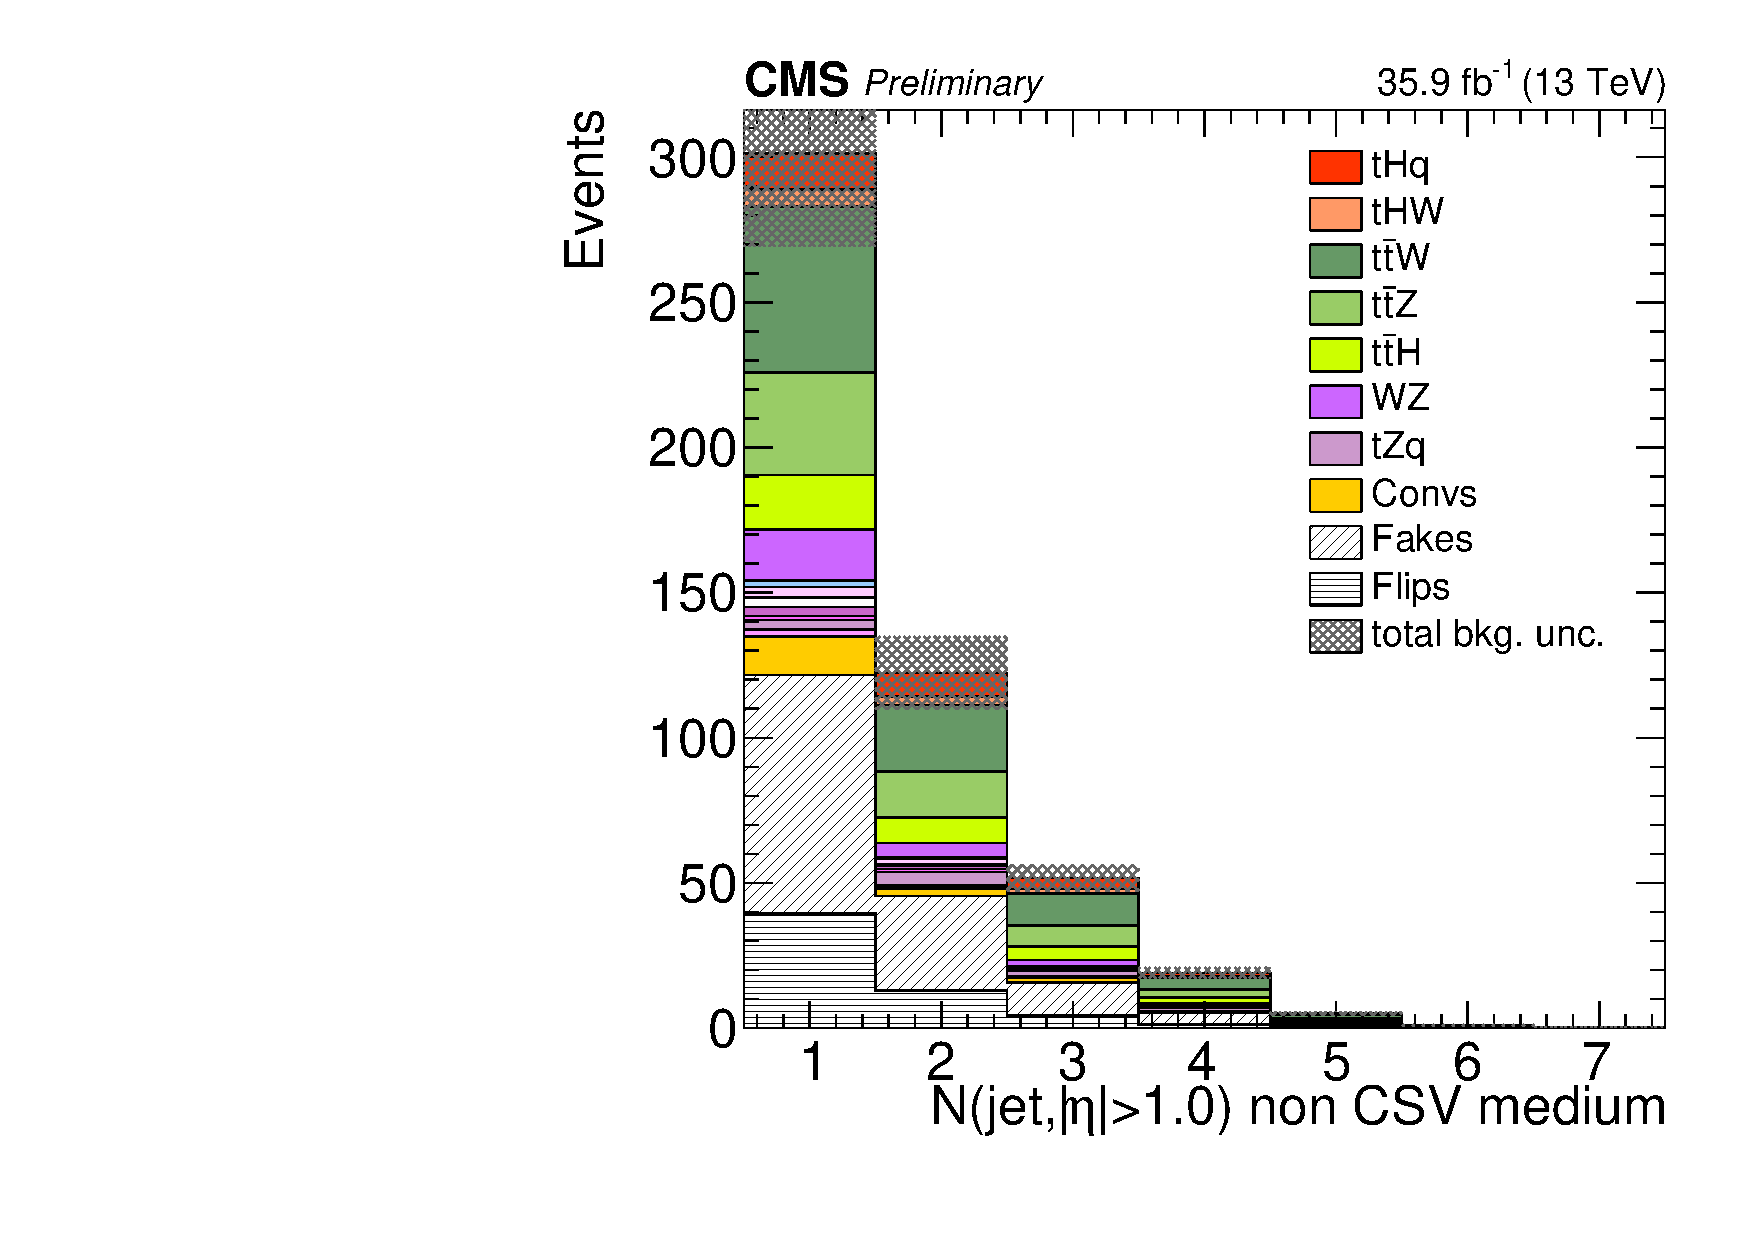
\includegraphics[width=0.245\textwidth]{nJetEta1.pdf}
 \includegraphics[width=0.245\textwidth]{totCharge.pdf}
\caption[Input variables to the BDT for signal discrimination not normalized.]{Distributions of input variables to the BDT for signal discrimination, three lepton channel.} 
\label{fig:input_vars_3l}
\end{figure}    

%% \begin{figure} [!h]
%%   \centering
%%   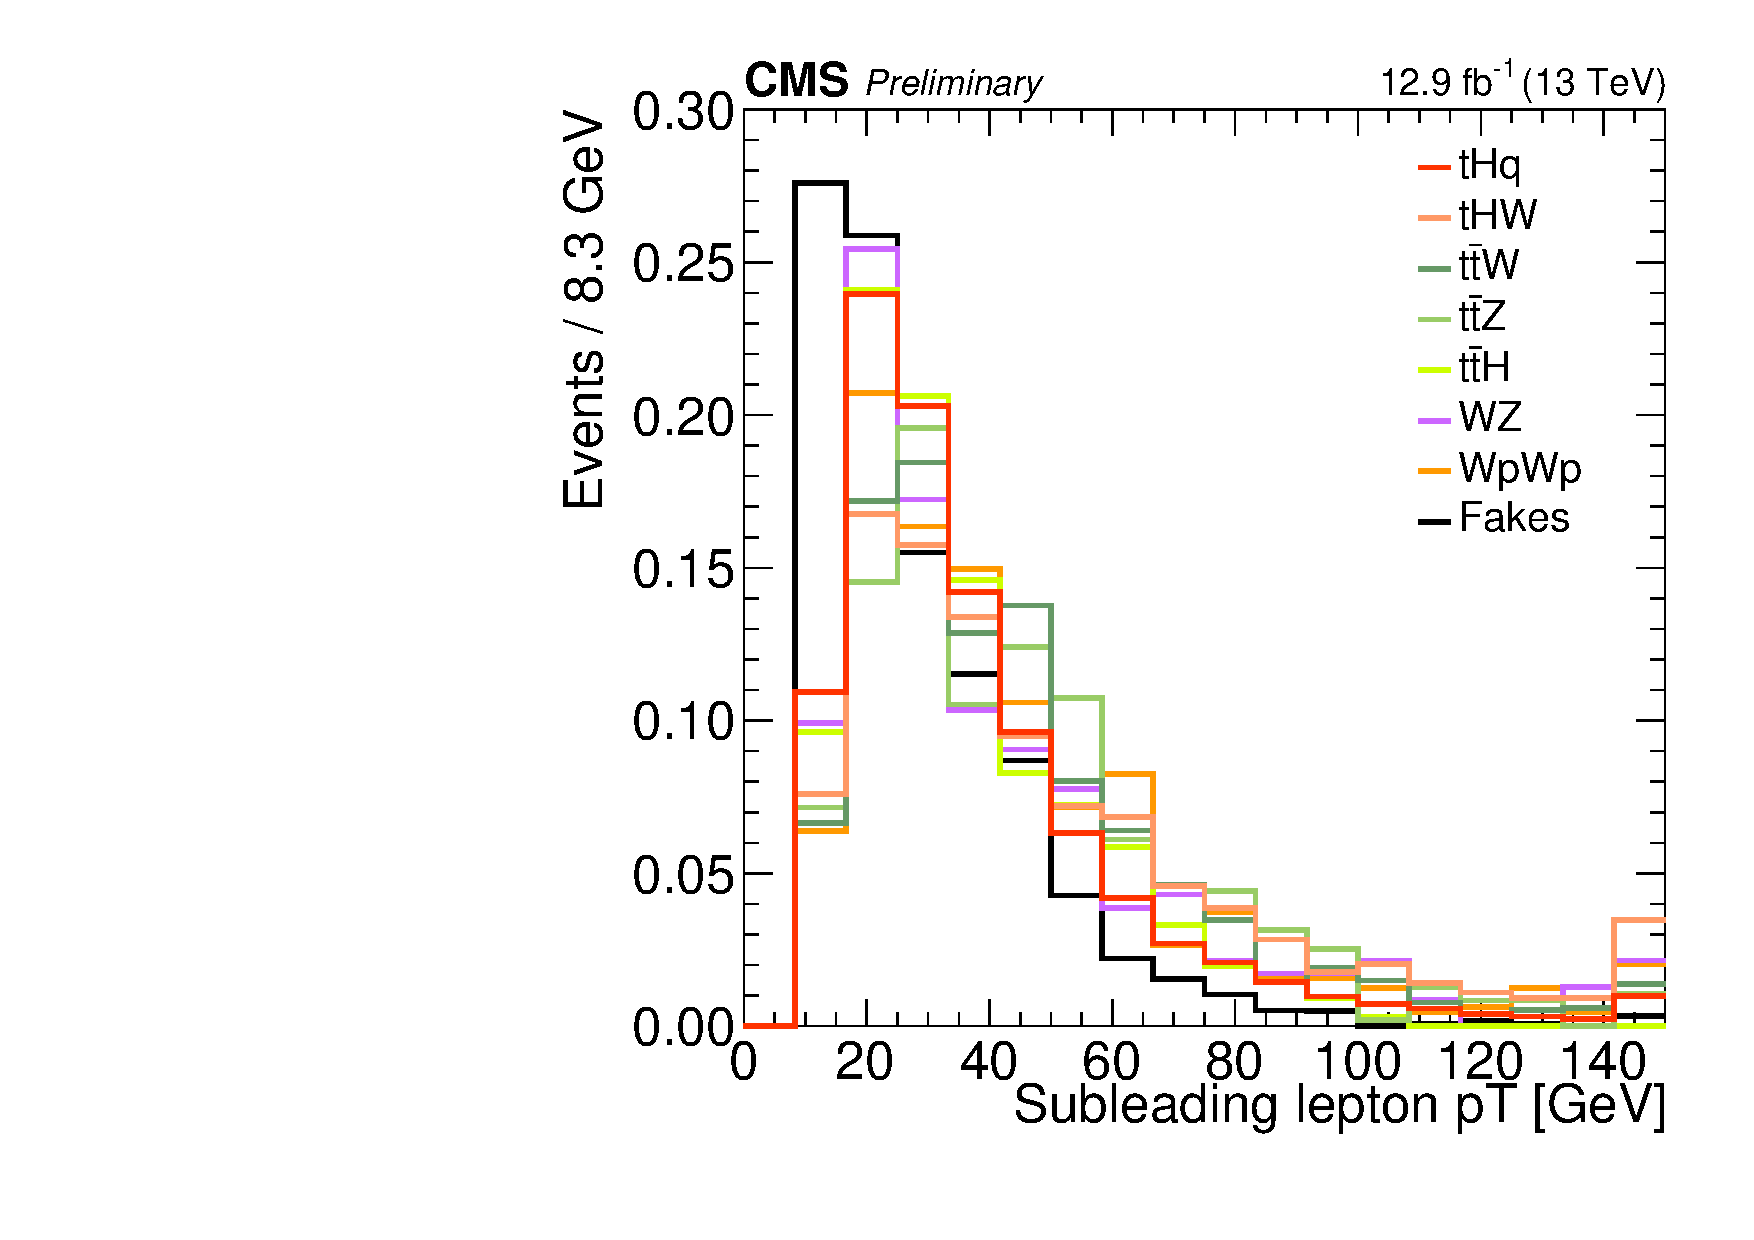
\includegraphics[width=0.245\textwidth]{Lep2Pt_mumu.pdf} 
%%   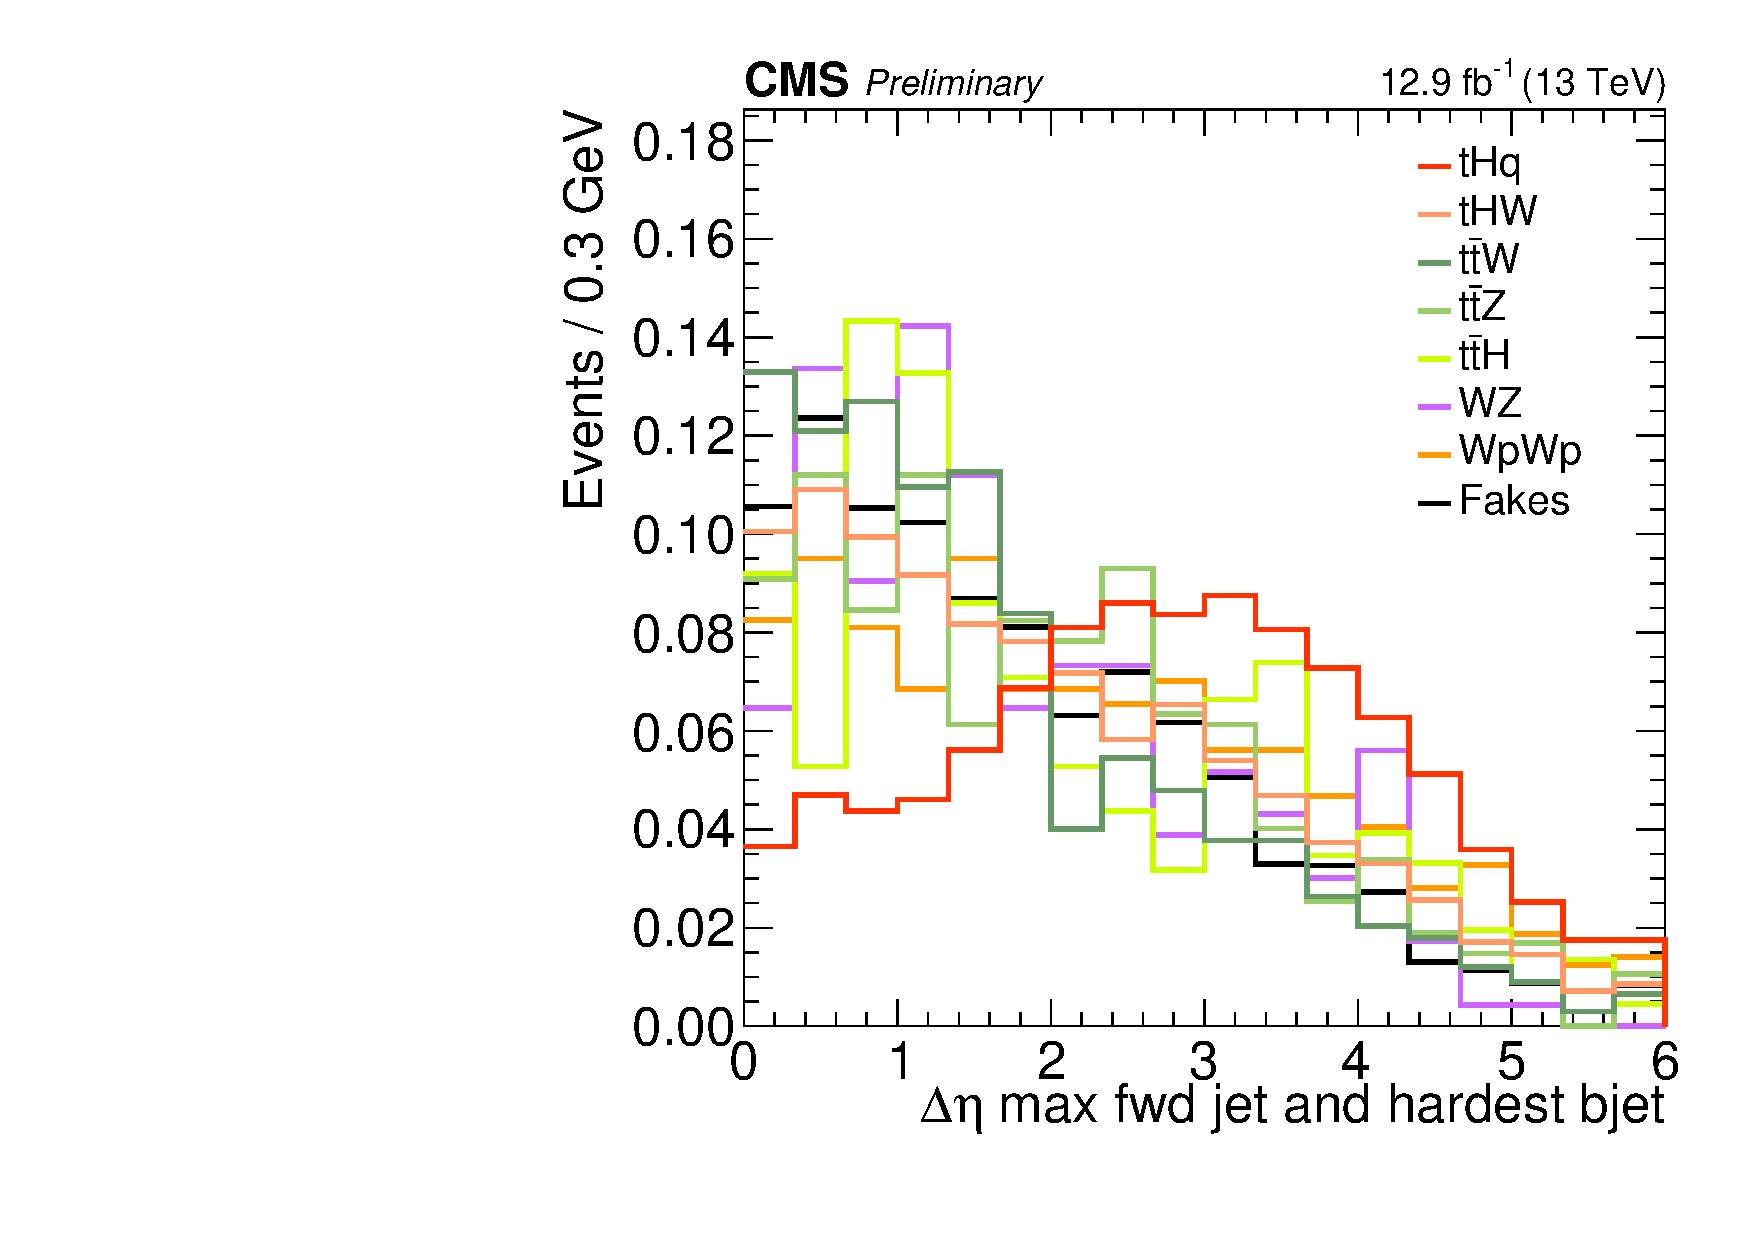
\includegraphics[width=0.245\textwidth]{dEtaFwdJetBJet_mumu.pdf}
%%   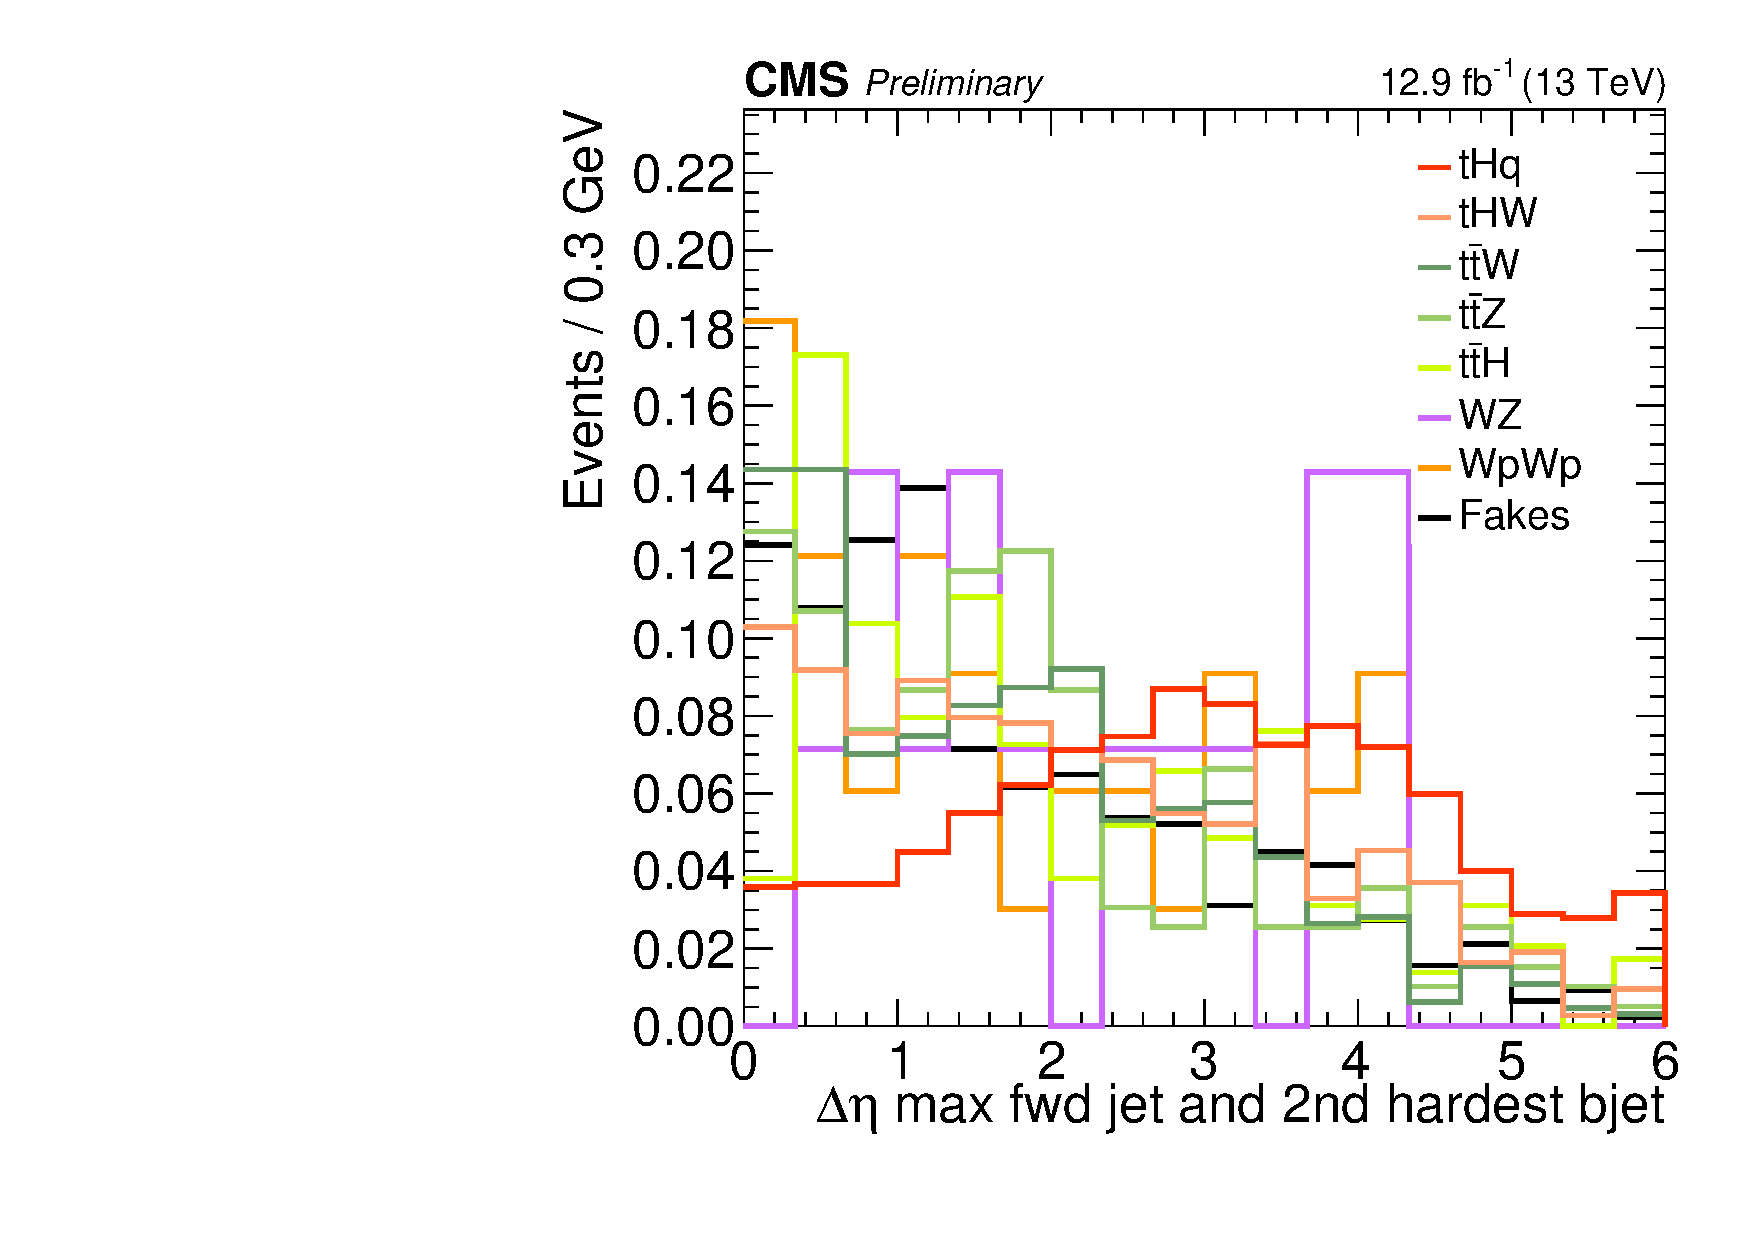
\includegraphics[width=0.245\textwidth]{dEtaFwdJet2BJet_mumu.pdf}
%%   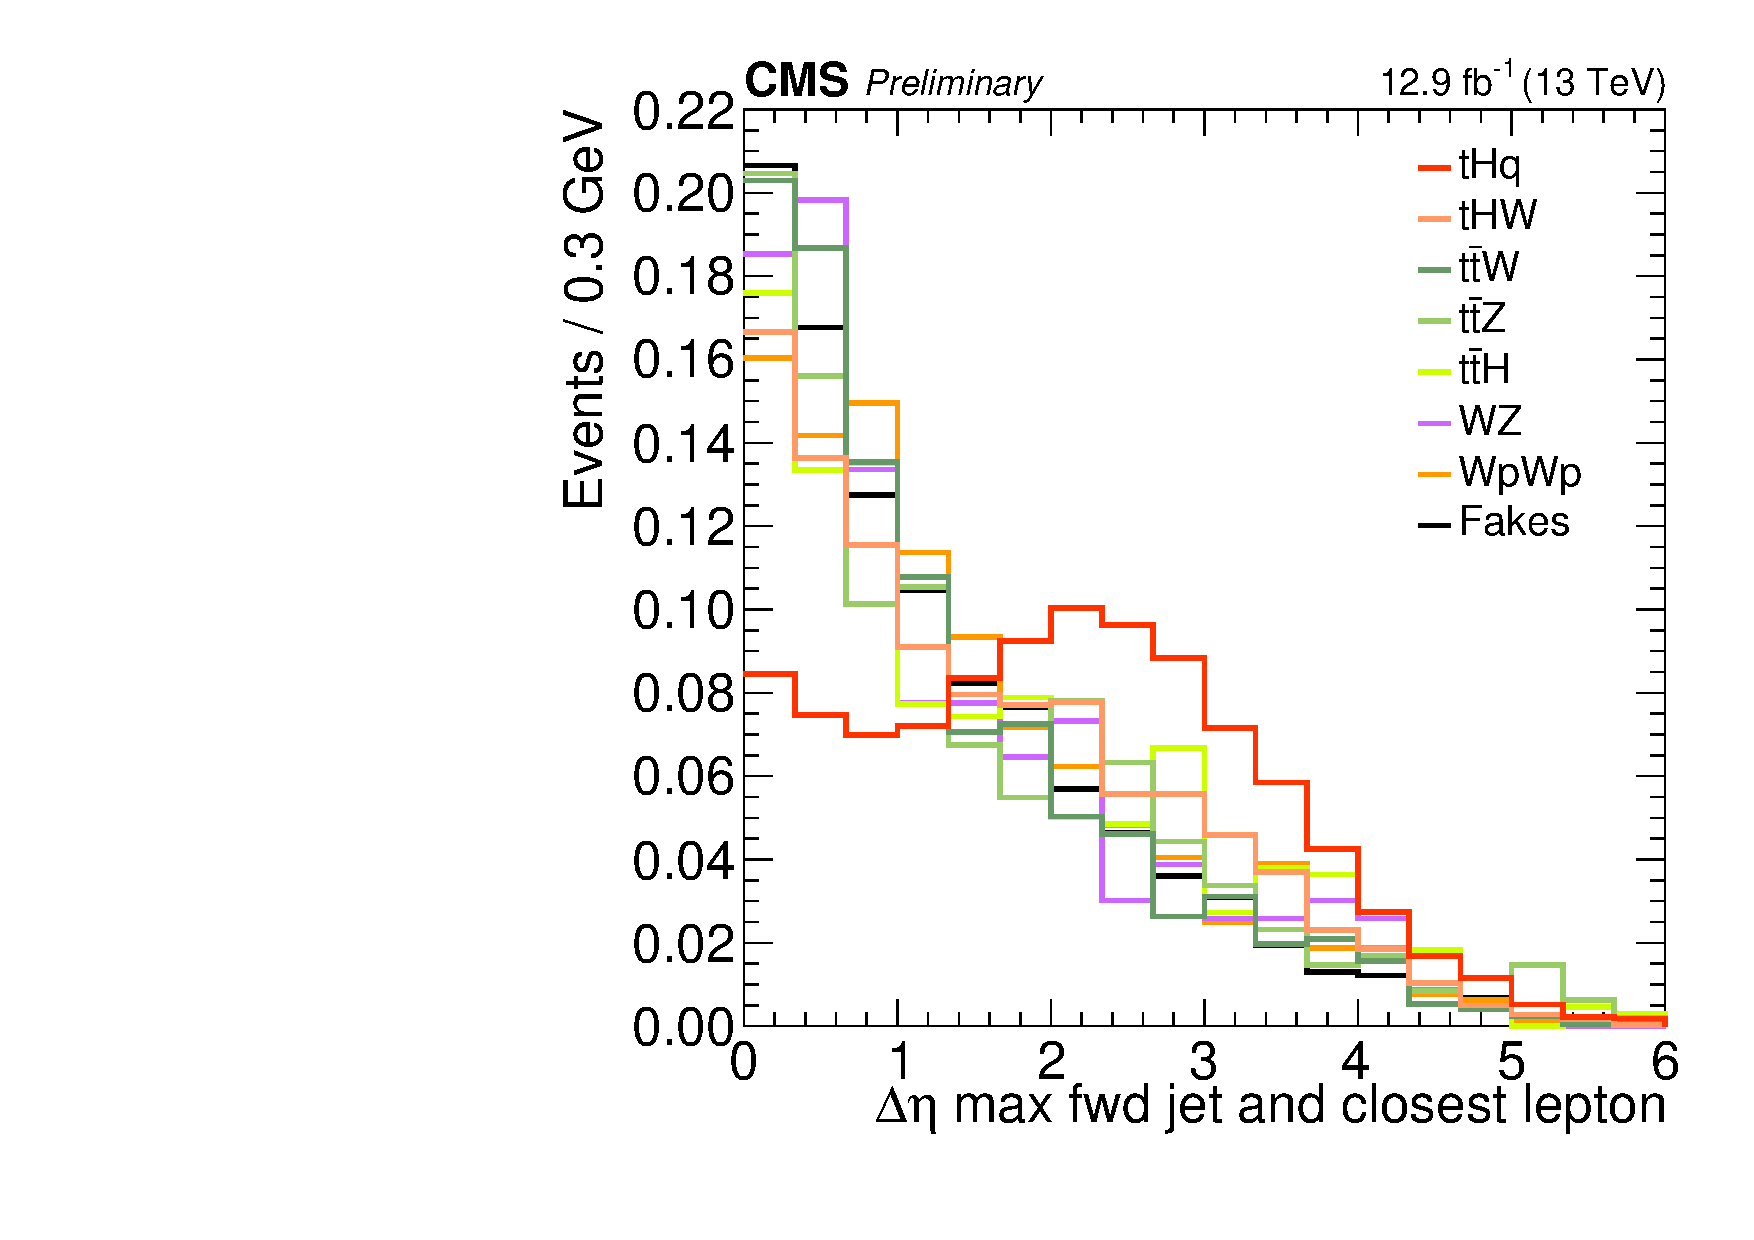
\includegraphics[width=0.245\textwidth]{dEtaFwdJetClosestLep_mumu.pdf} \\
%%   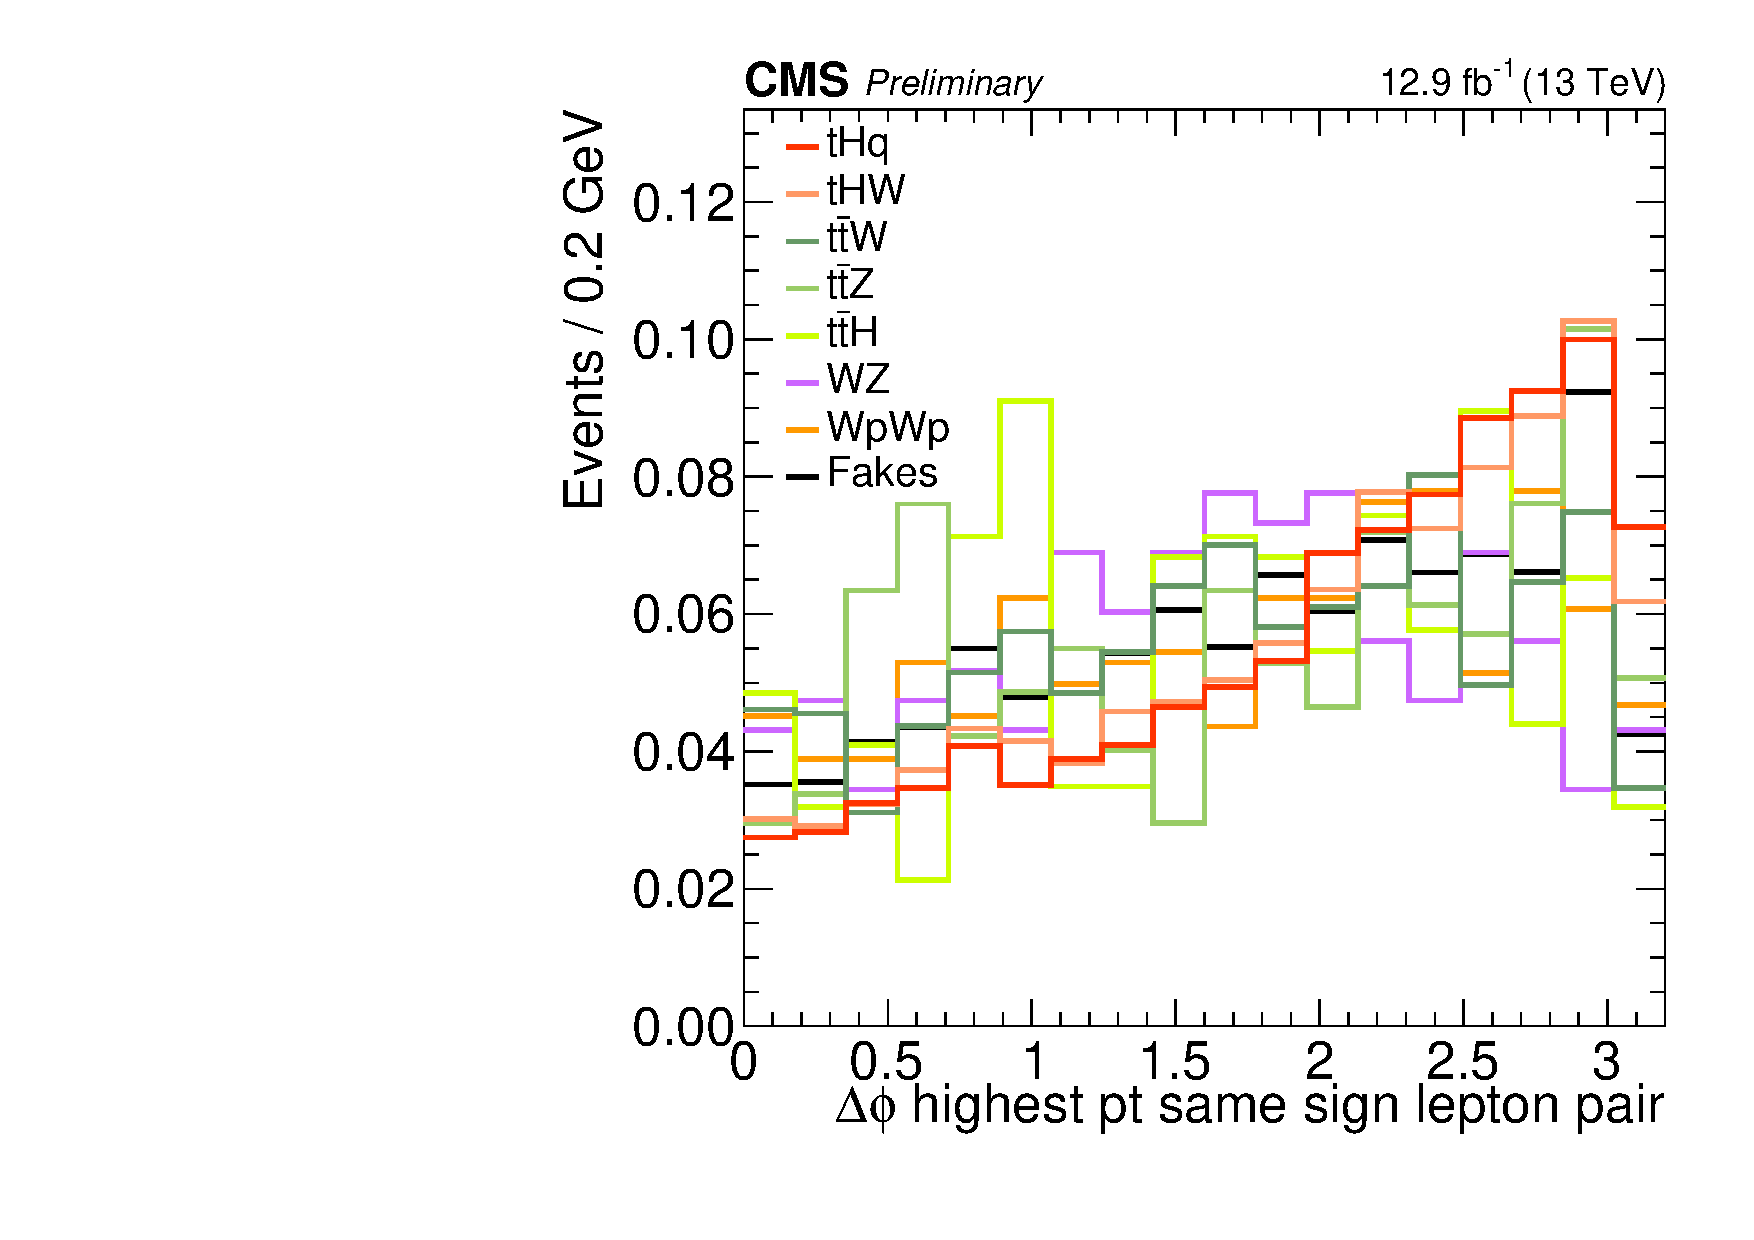
\includegraphics[width=0.245\textwidth]{dPhiHighestPtSSPair_mumu.pdf}
%%   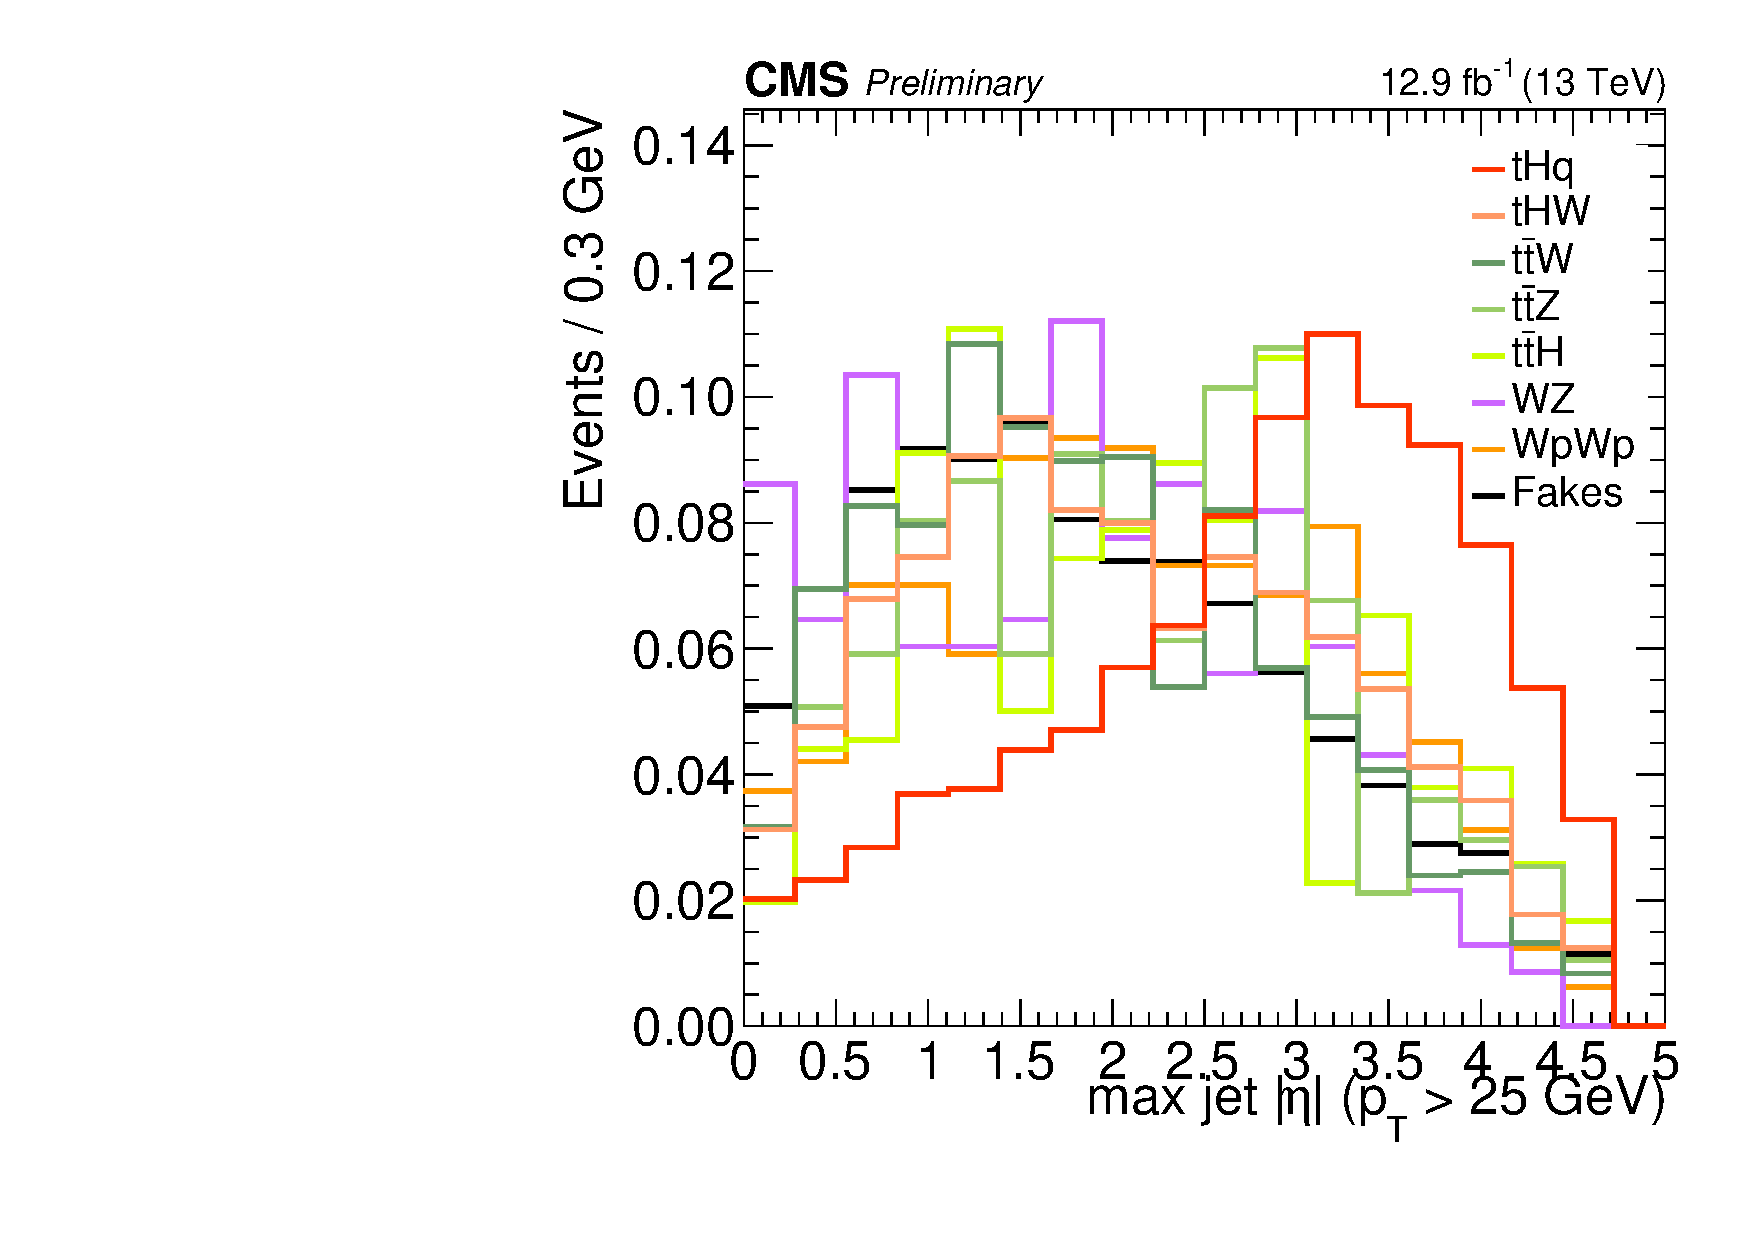
\includegraphics[width=0.245\textwidth]{maxEtaJet25_mumu.pdf}
%%   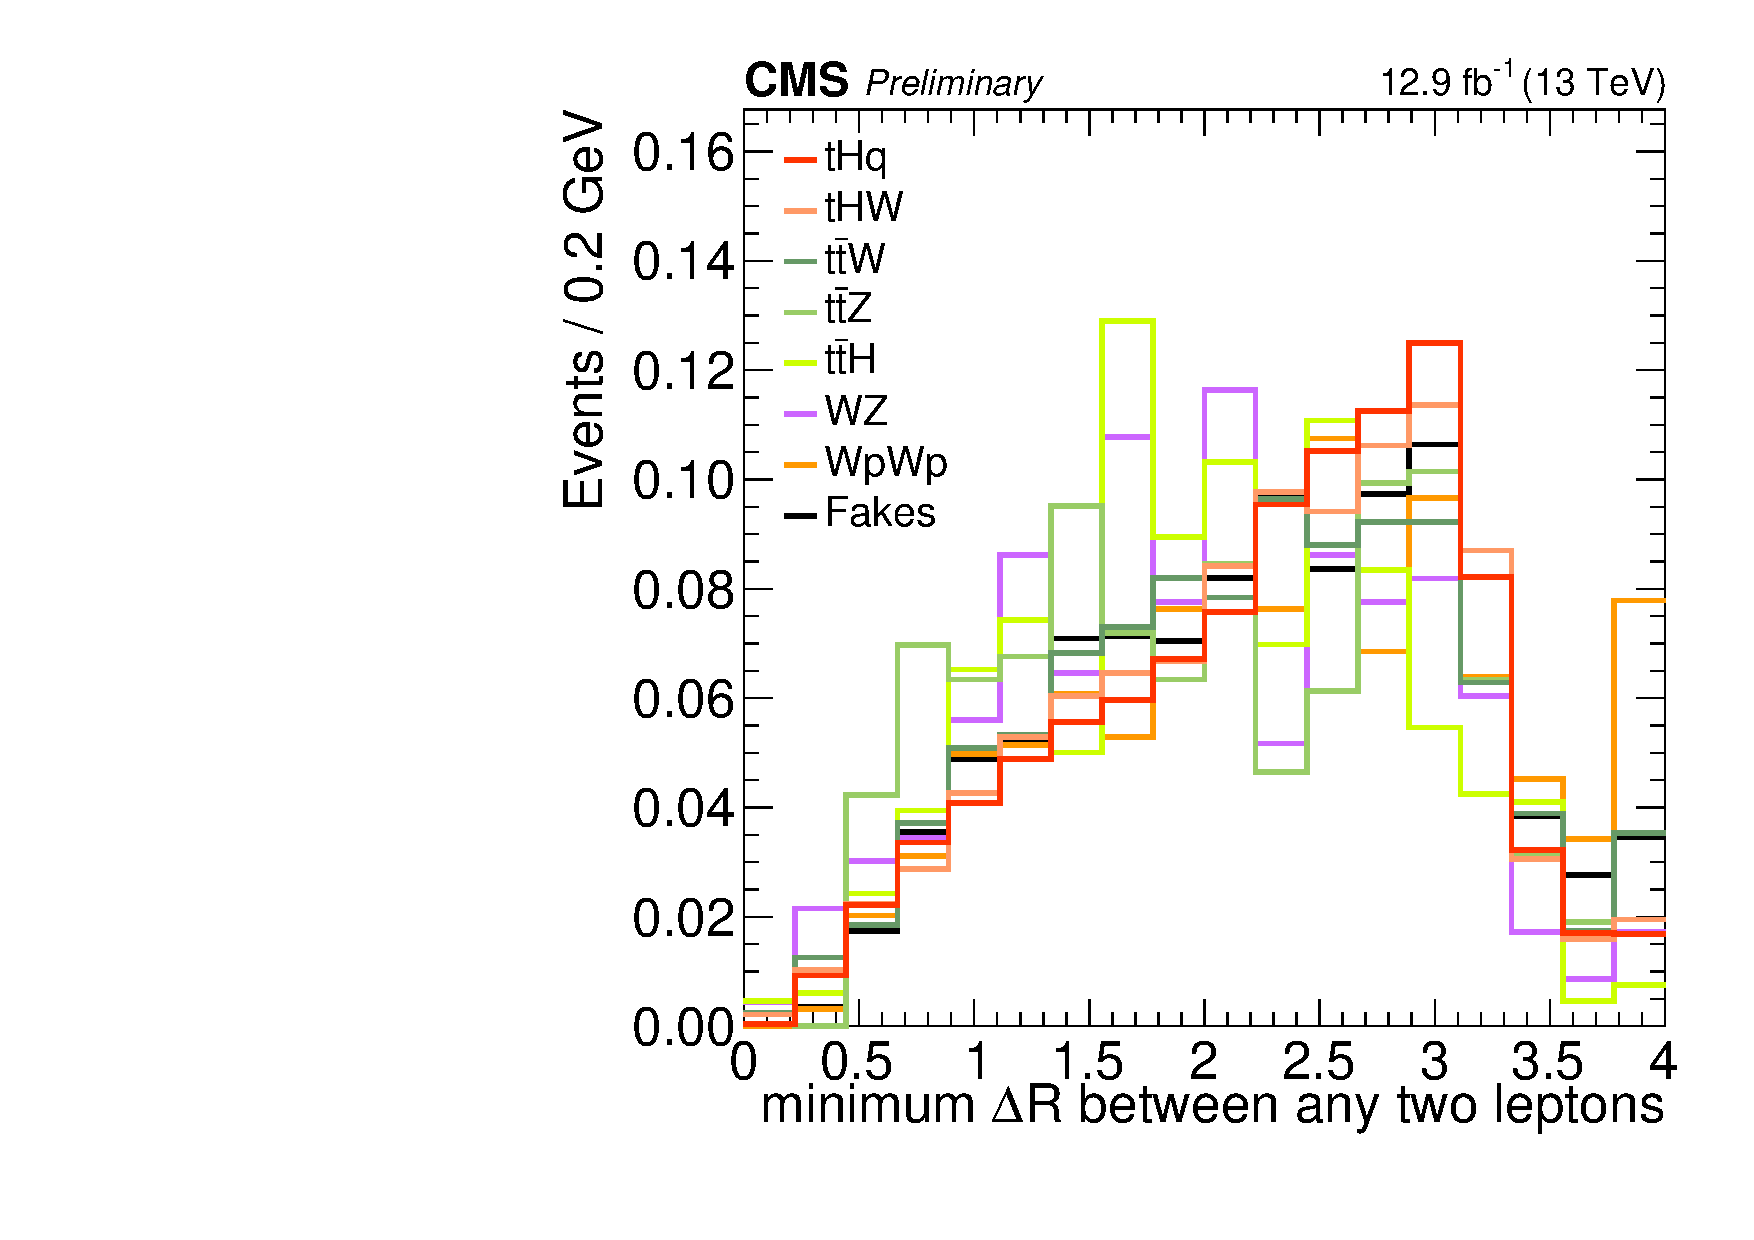
\includegraphics[width=0.245\textwidth]{minDRll_mumu.pdf}
%%   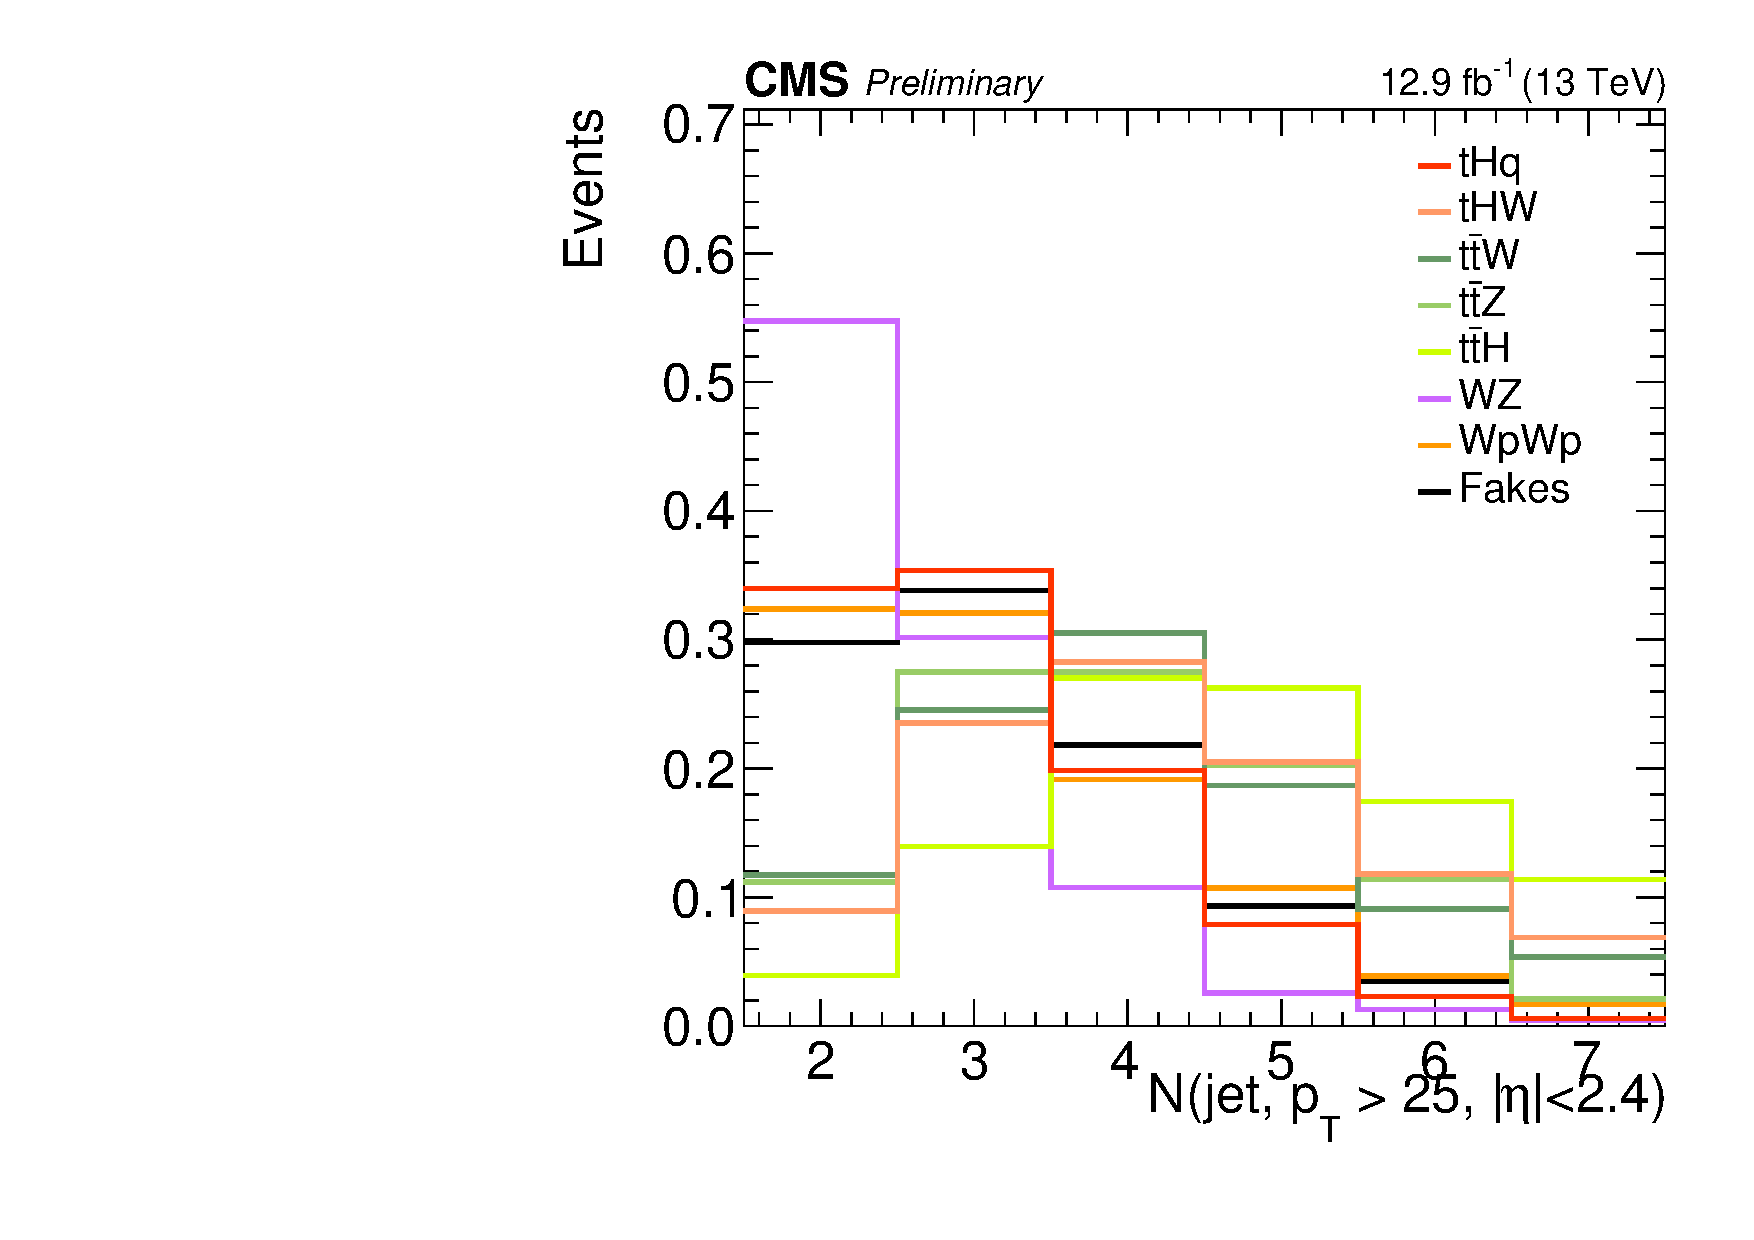
\includegraphics[width=0.245\textwidth]{nJet25_mumu.pdf} \\
%%   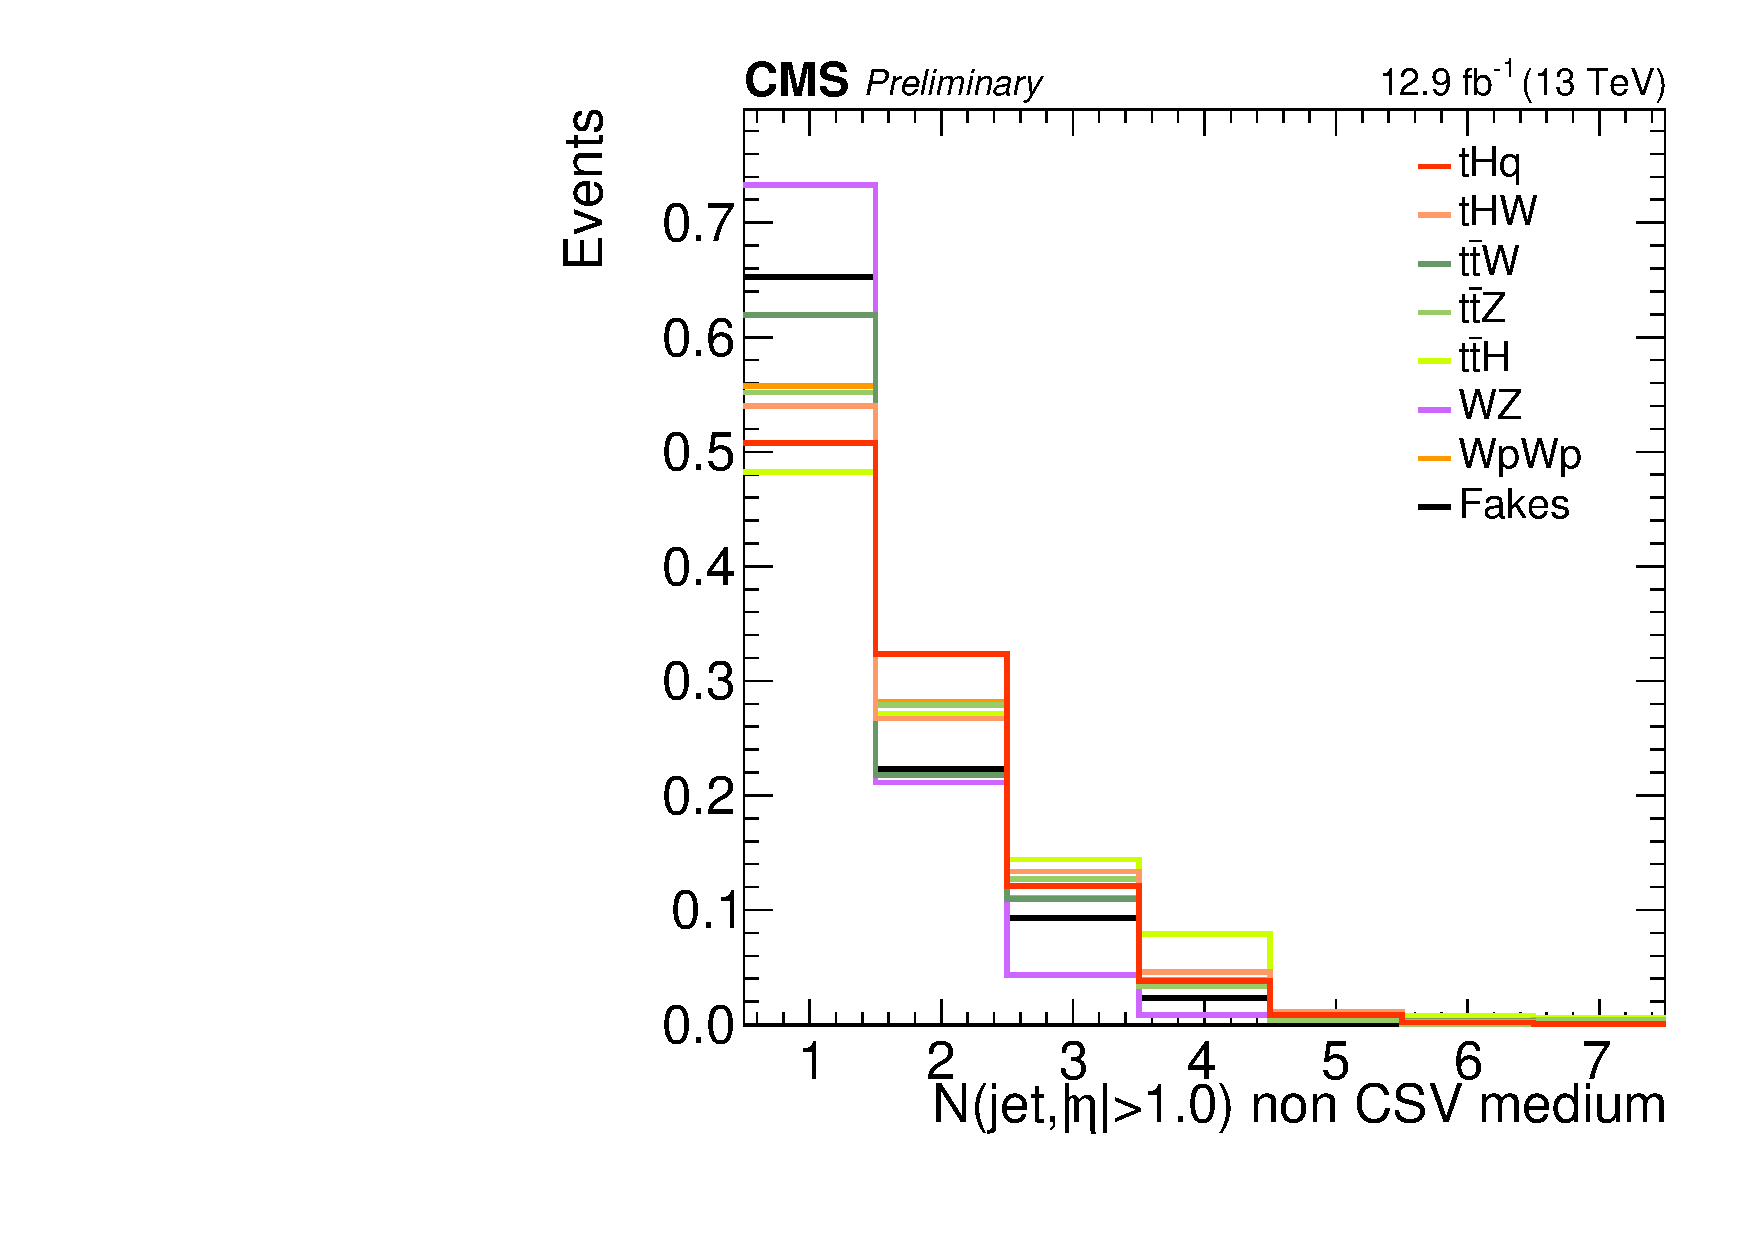
\includegraphics[width=0.245\textwidth]{nJetEta1_mumu.pdf}
%%   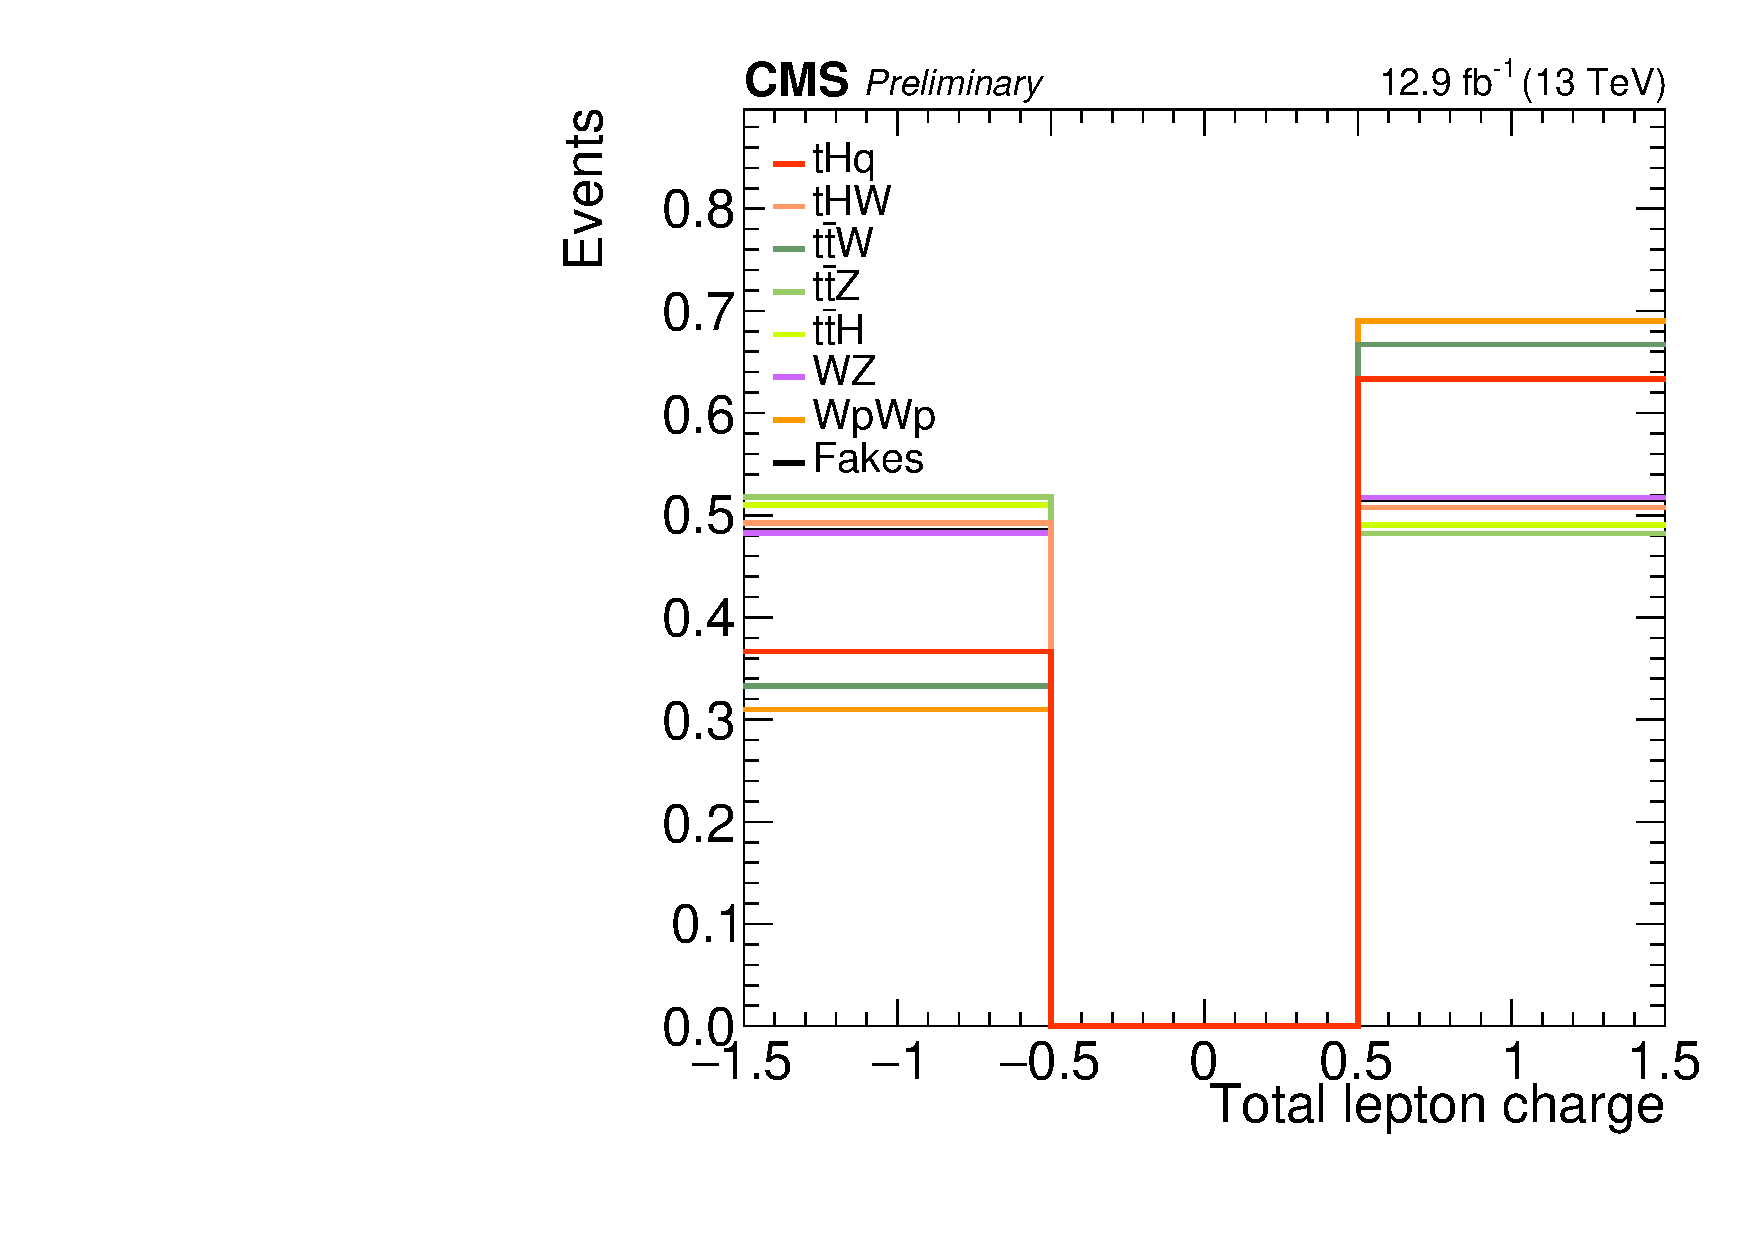
\includegraphics[width=0.245\textwidth]{totCharge_mumu.pdf}
%%  \caption{Distributions of input variables to the BDT for signal discrimination, two lepton same sign channel.}
%% \label{fig:input_vars_2lss}
%% \end{figure}    

The MVA analysis consist of two stages: first a ``training'' where the MVA method is trained to discriminate between simulated signal and background events, then a ``test'' stage where the trained algorithm is used to classify different events from the samples. The sample is obtained from a pre-selection (see Tab.~\ref{tab:evsel} with pre-selection cuts). Figures~\ref{mva_input_tt} show the input variables distributions as seen by the MVA algorithm. Note that in contrast to the distributions in Fig.~\ref{fig:input_vars_3l} only the main backgrounds (\ttbar\ from simulation, \ttV) are included.

\begin{figure} [!h]
  \centering
  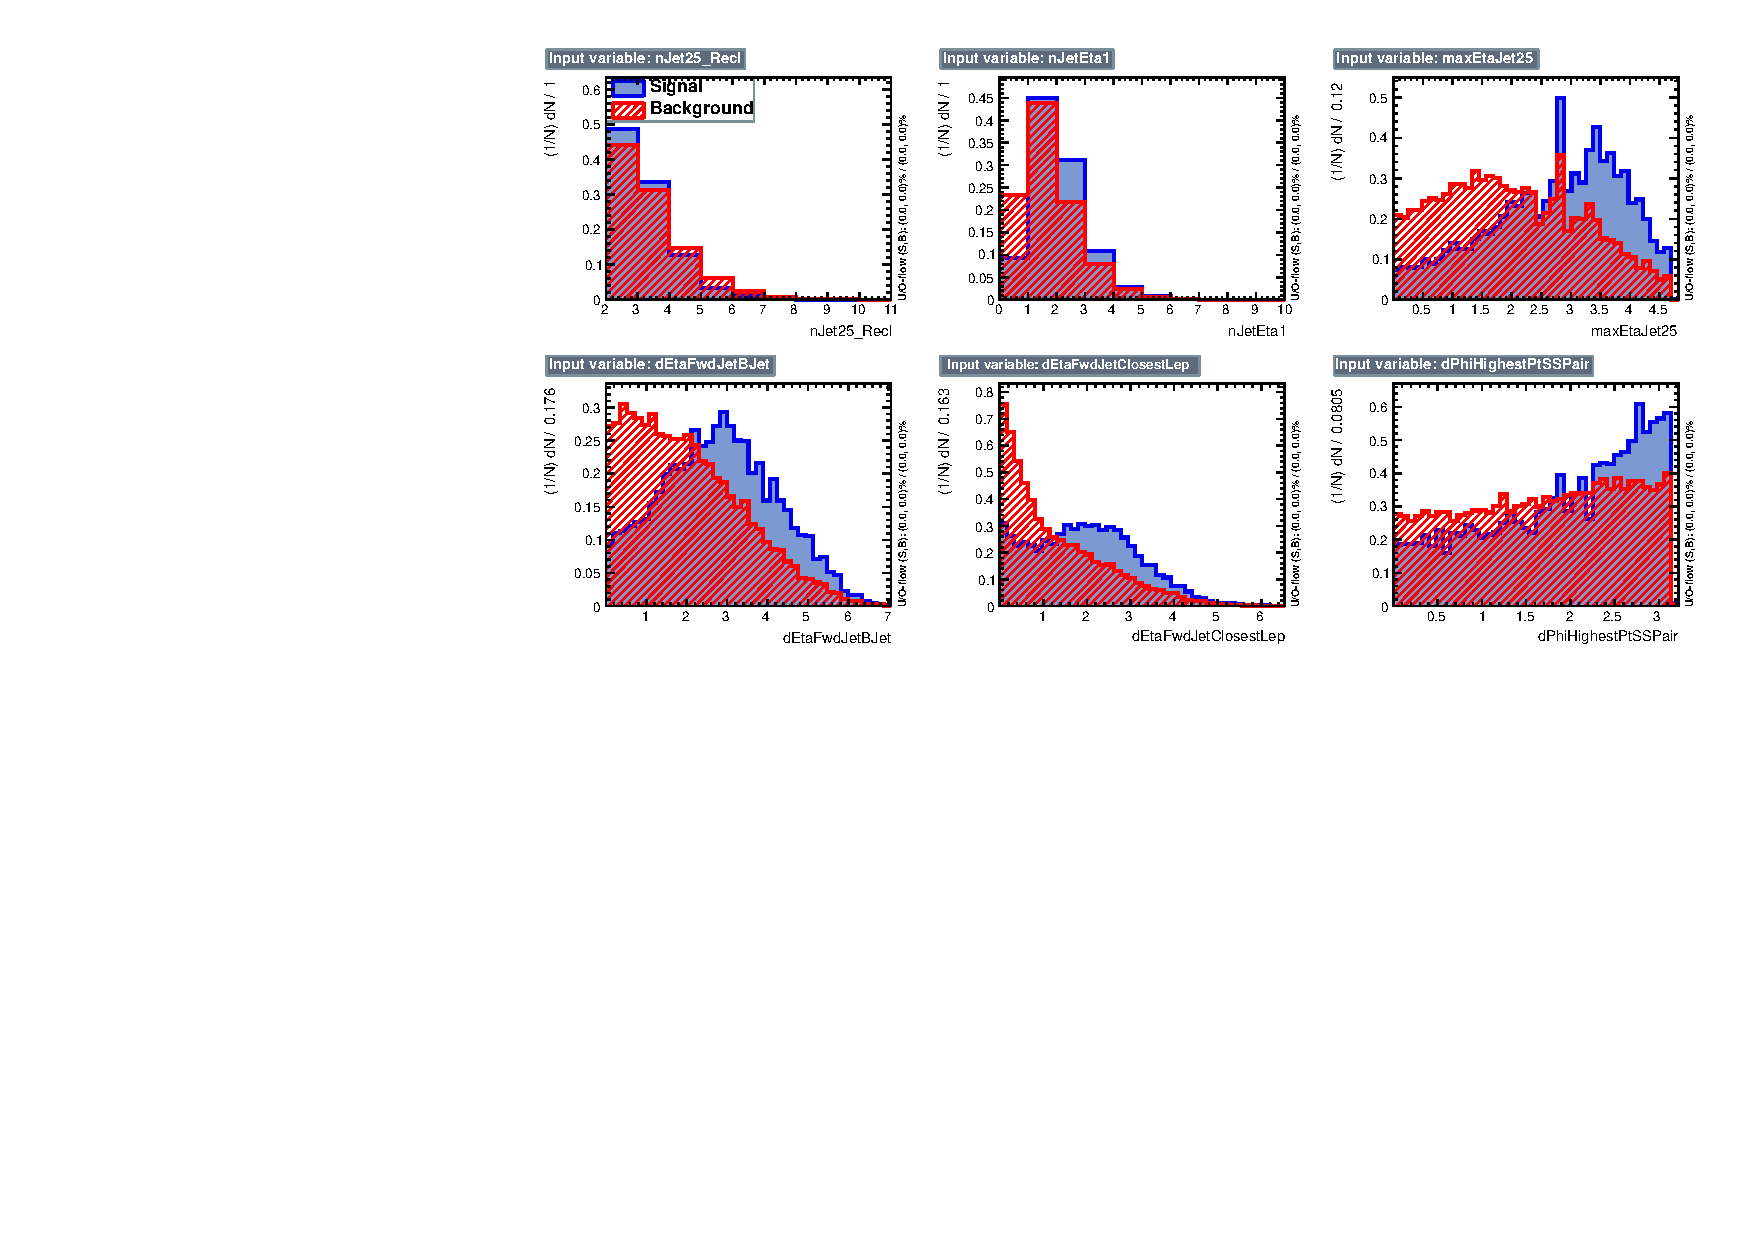
\includegraphics[width=\textwidth]{mva_input1_tt.pdf}
  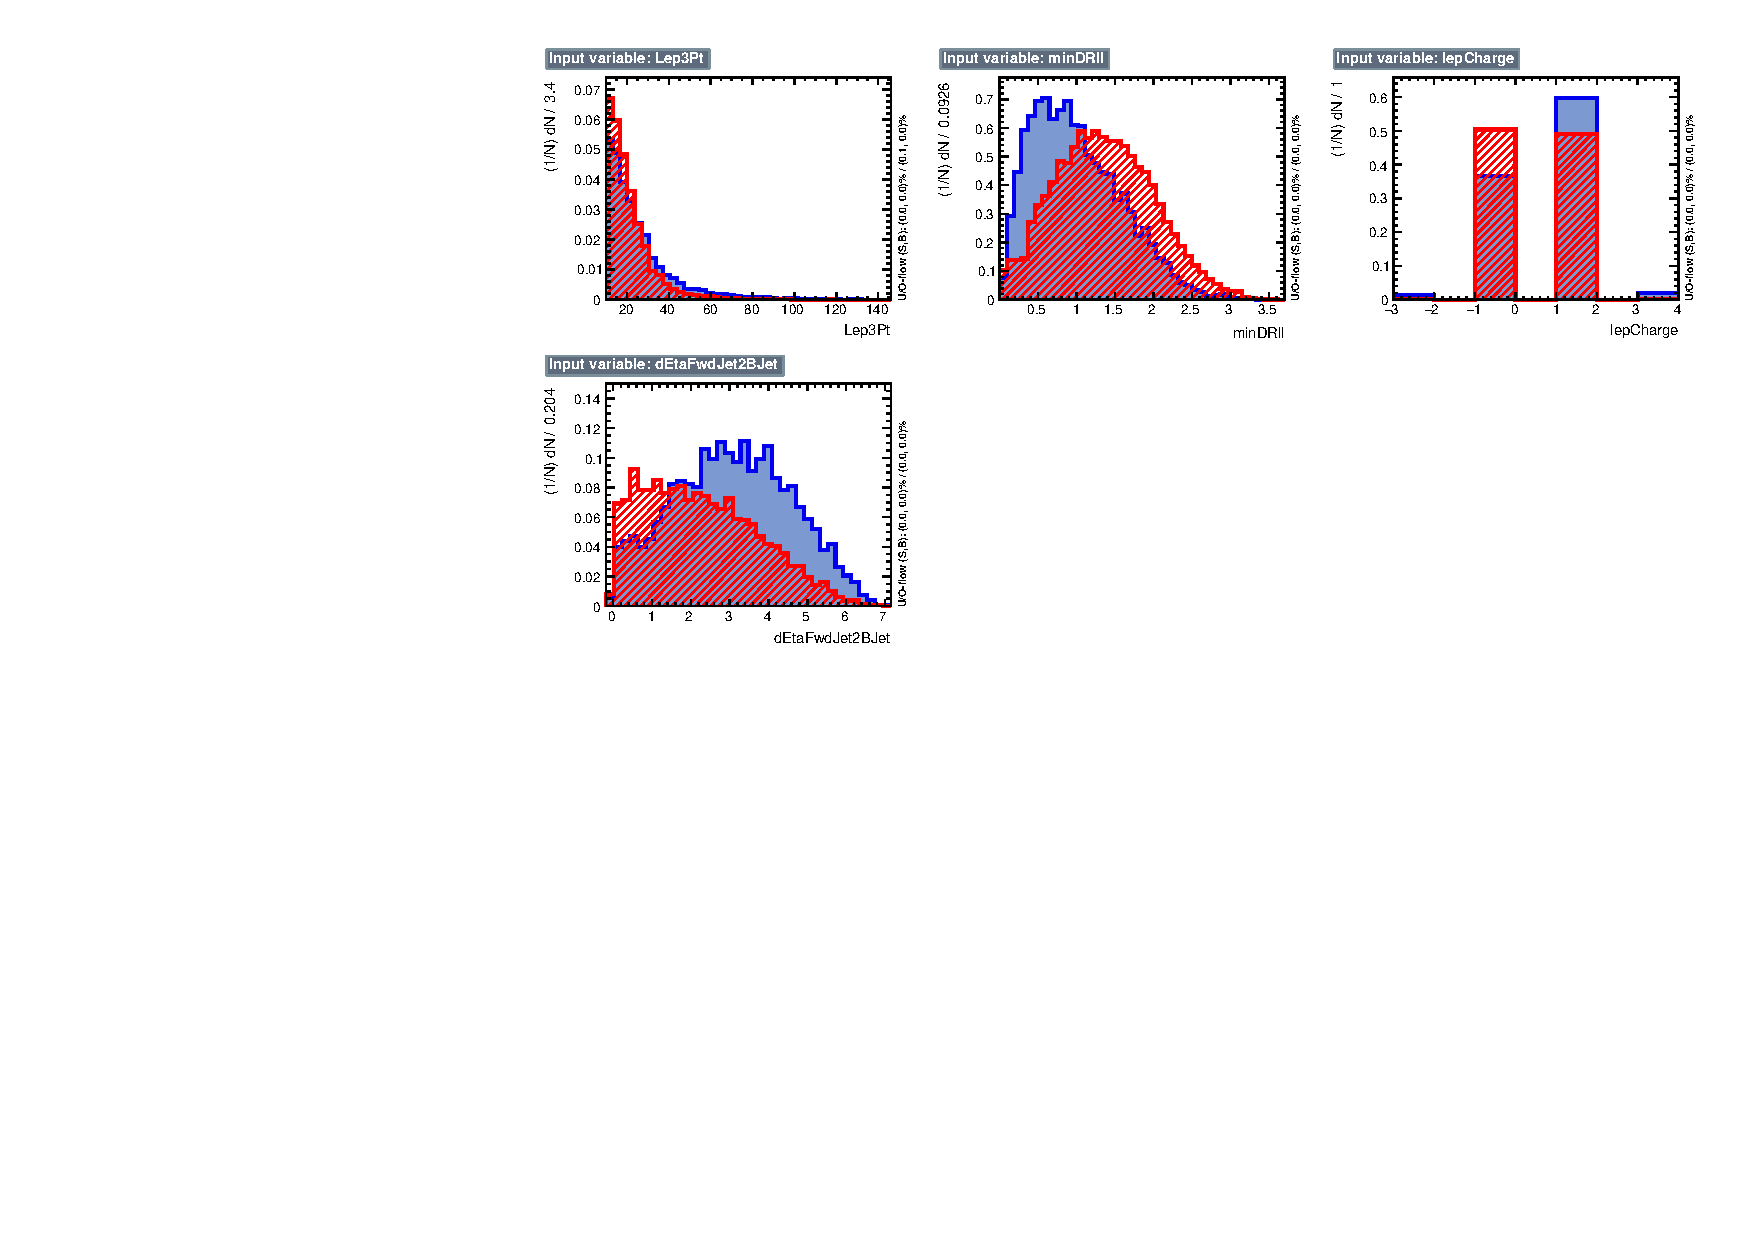
\includegraphics[width=\textwidth]{mva_input2_tt.pdf}
\caption[BDT inputs as seen by TMVA against \ttbar.]{BDT inputs as seen by TMVA (signal, in blue, is \tHq, background, in red, is \ttbar) for the three lepton channel, discriminated against \ttbar\ (fakes) background.} 
\label{mva_input_tt}
\end{figure}

\begin{figure} [!h]
  \centering
  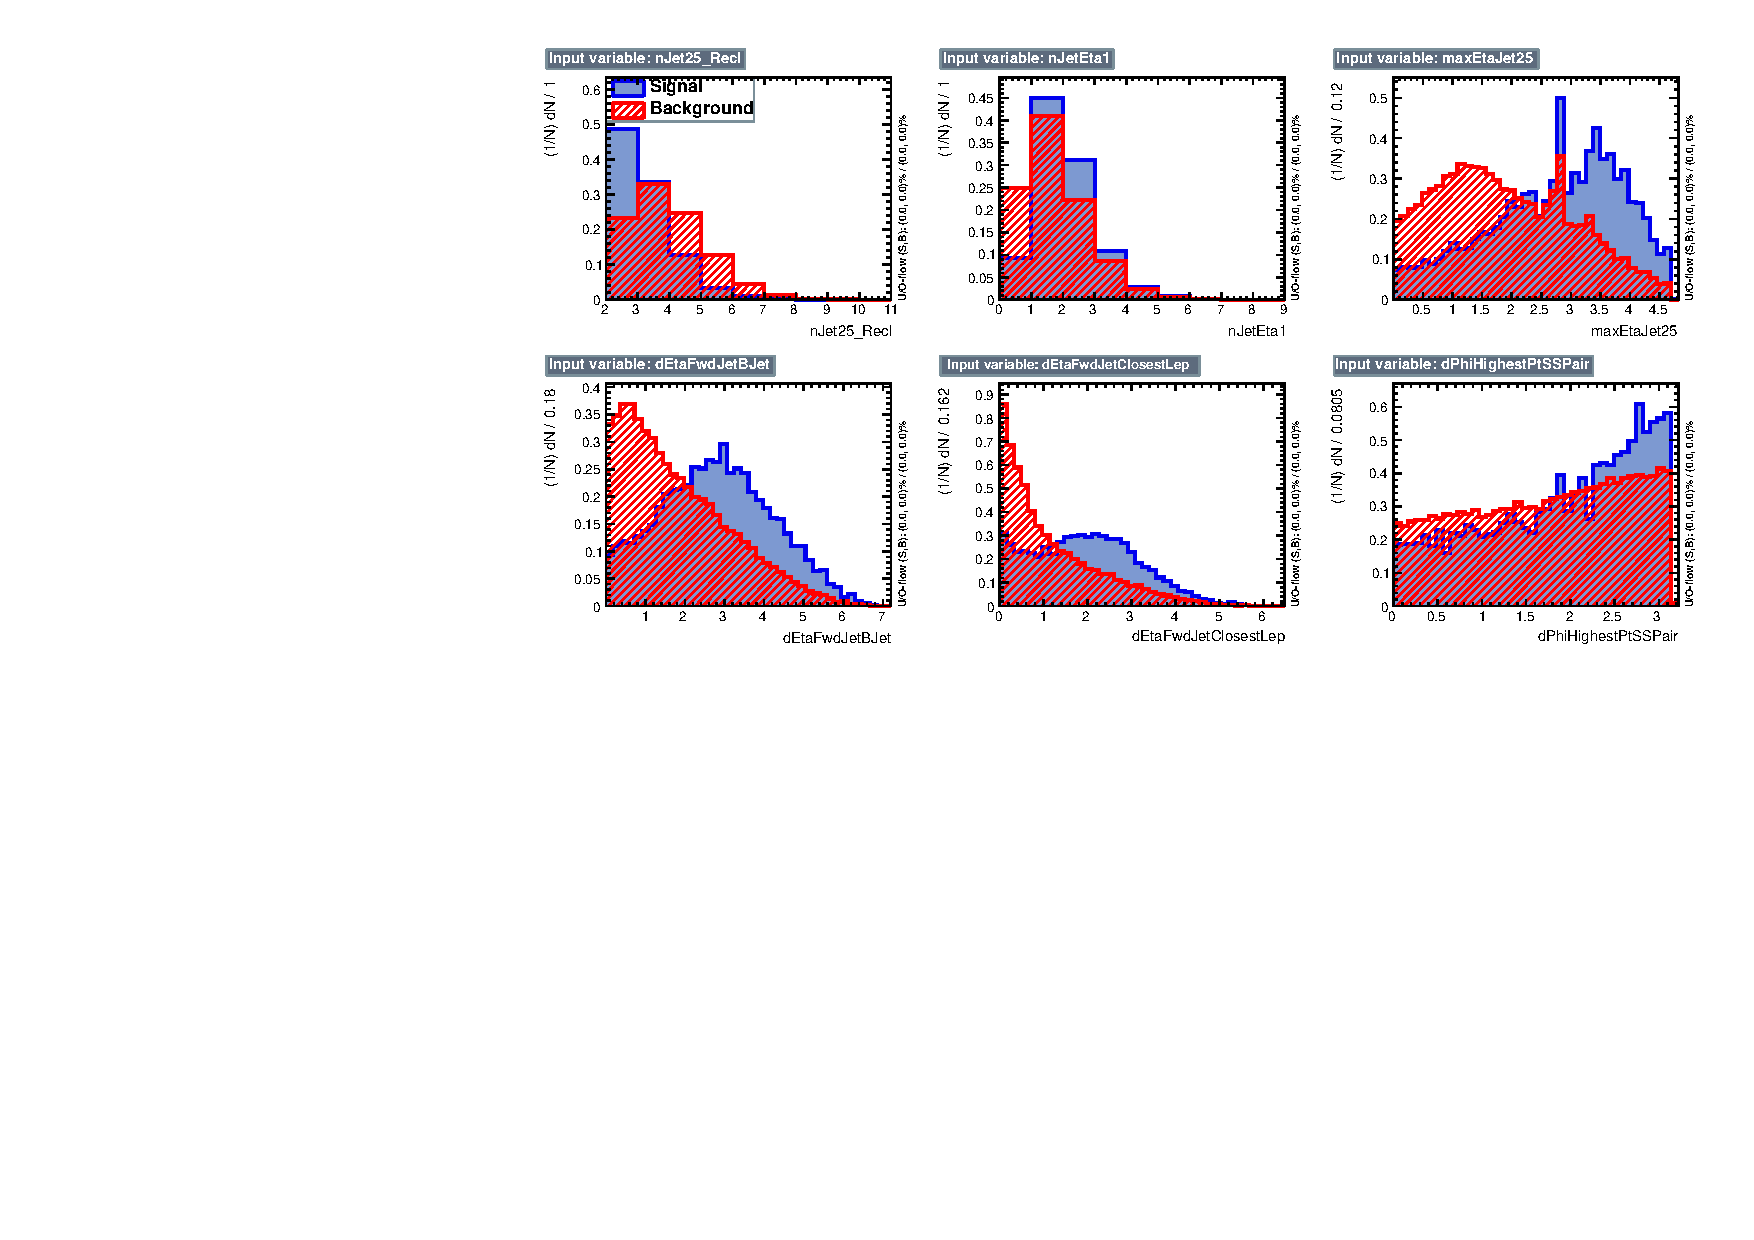
\includegraphics[width=\textwidth]{mva_input1_ttv.pdf}
  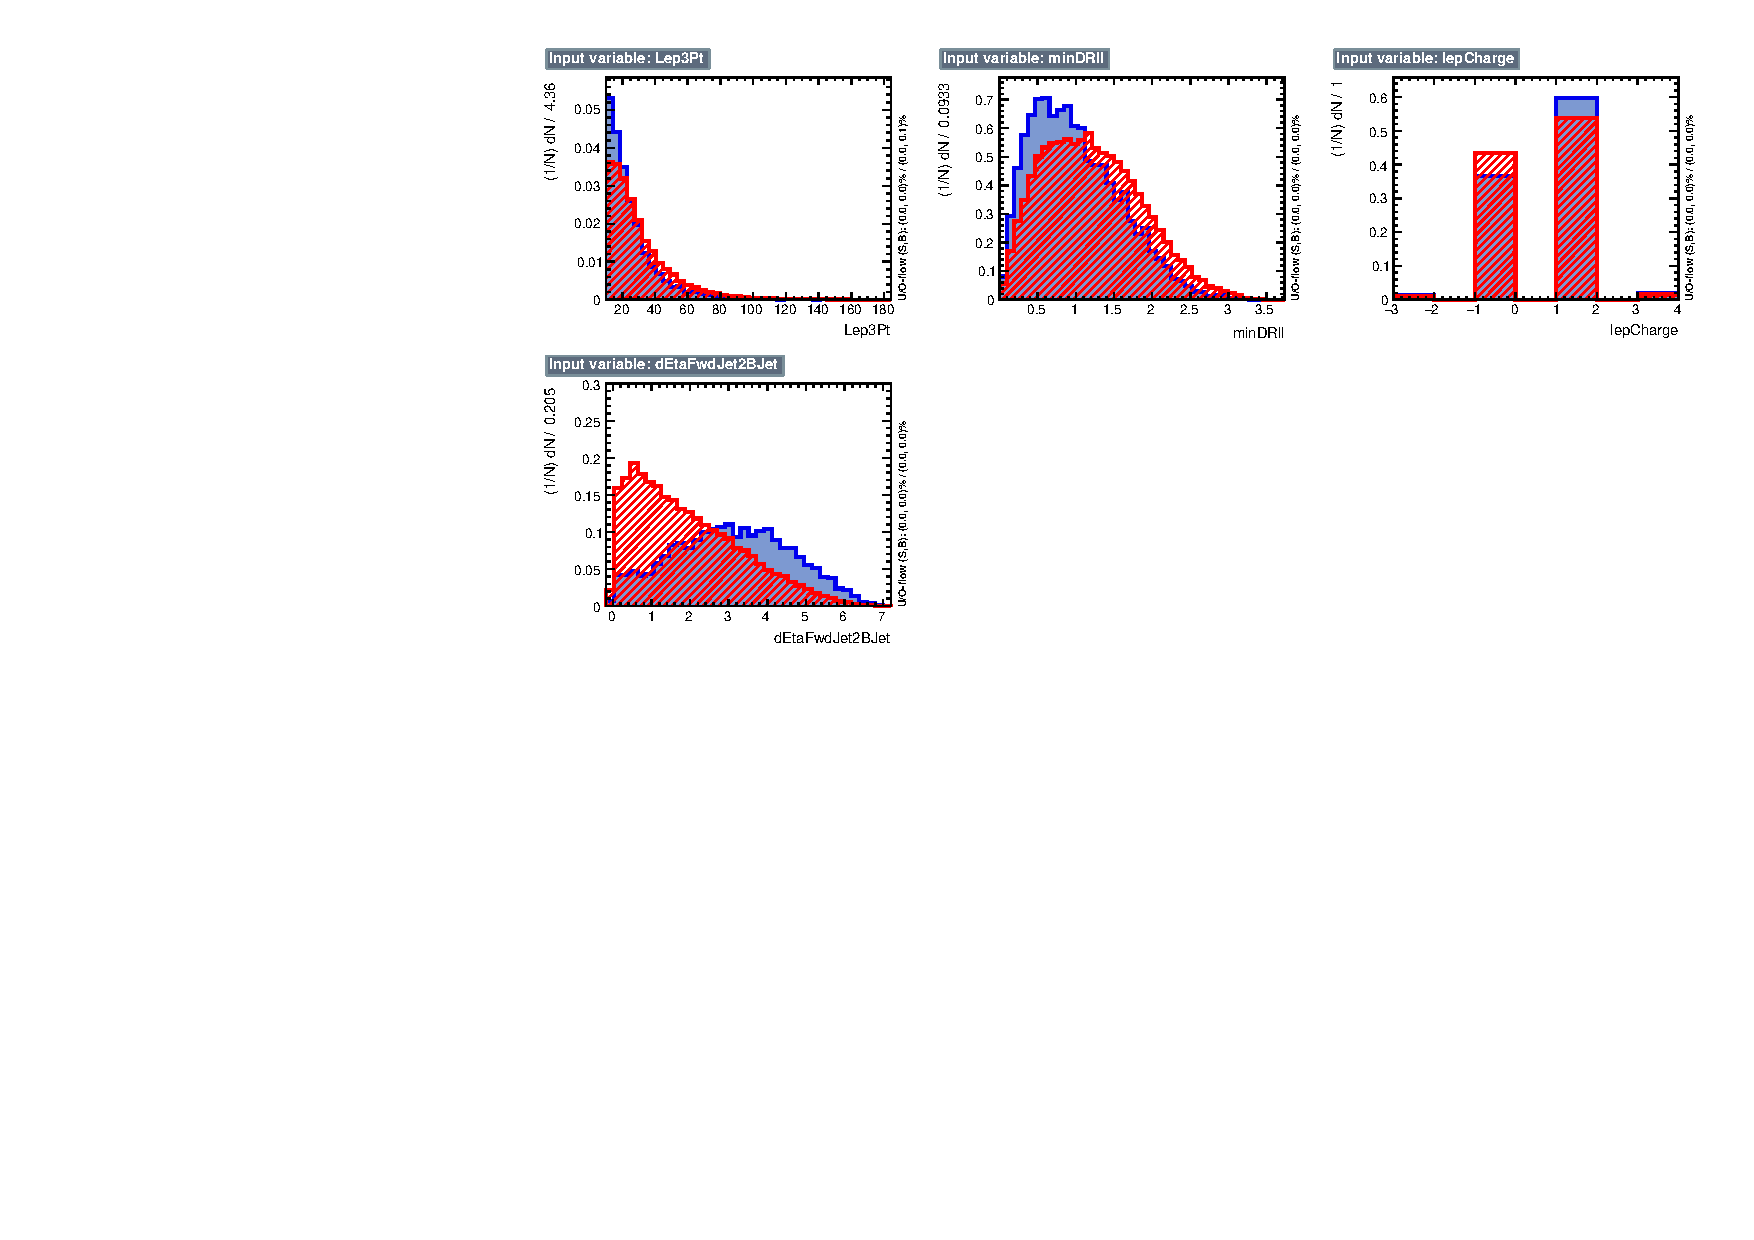
\includegraphics[width=\textwidth]{mva_input2_ttv.pdf}
\caption[BDT inputs as seen by TMVA against \ttV\ .]{BDT inputs as seen by TMVA (signal, in blue, is \tHq, background, in red, is \ttW+\ttZ) for the three lepton channel, discriminated against \ttV\ background.}                                                                                                                                                         
\label{mva_input_ttv}
\end{figure}

%% The input variables distributions for 2lss channel for signal against the \ttbar\ and \ttV\ are shown in Figure~\ref{mva_input_2lss_tt} and Figure~\ref{mva_input_2lss_ttv} respectively.
%% \begin{figure} [!h]
%%   \centering
%%   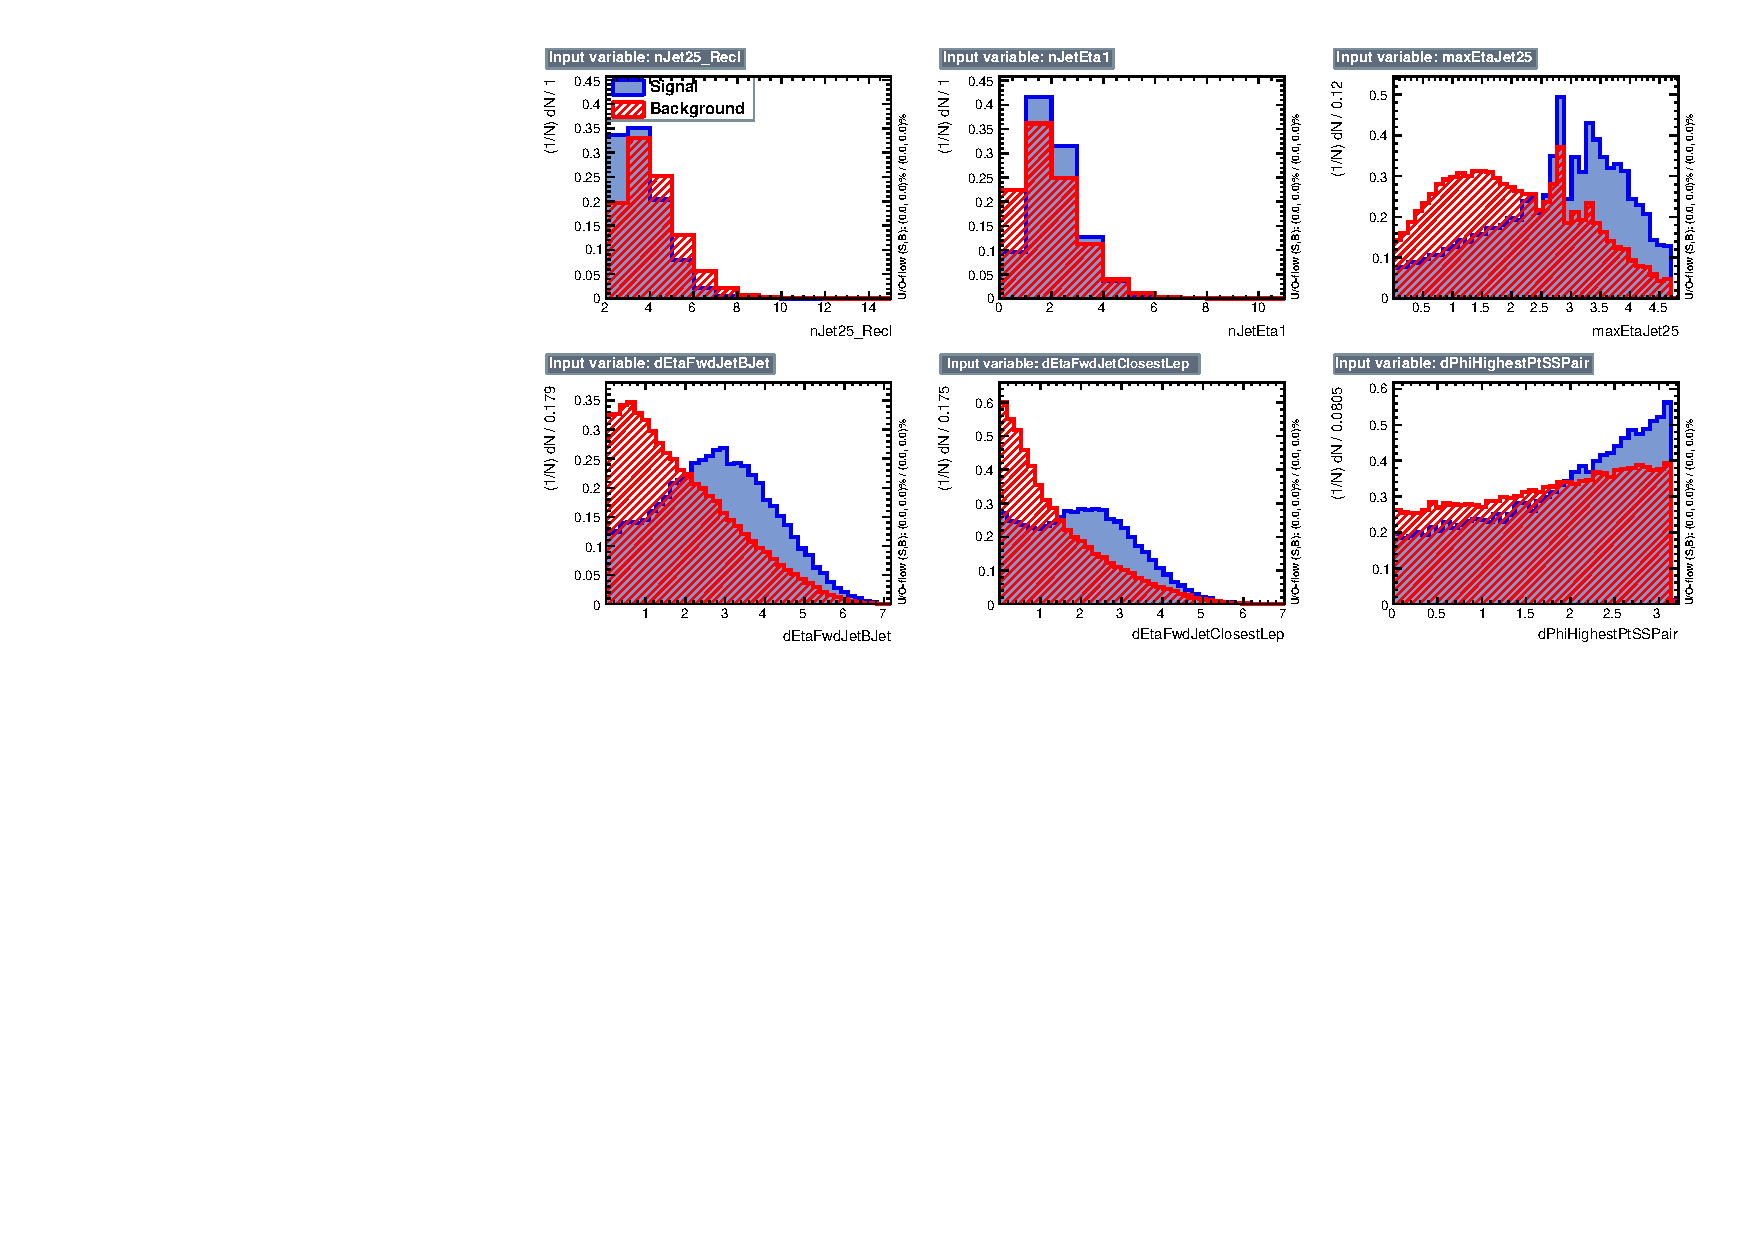
\includegraphics[width=\textwidth]{6var_tt.pdf}
%%   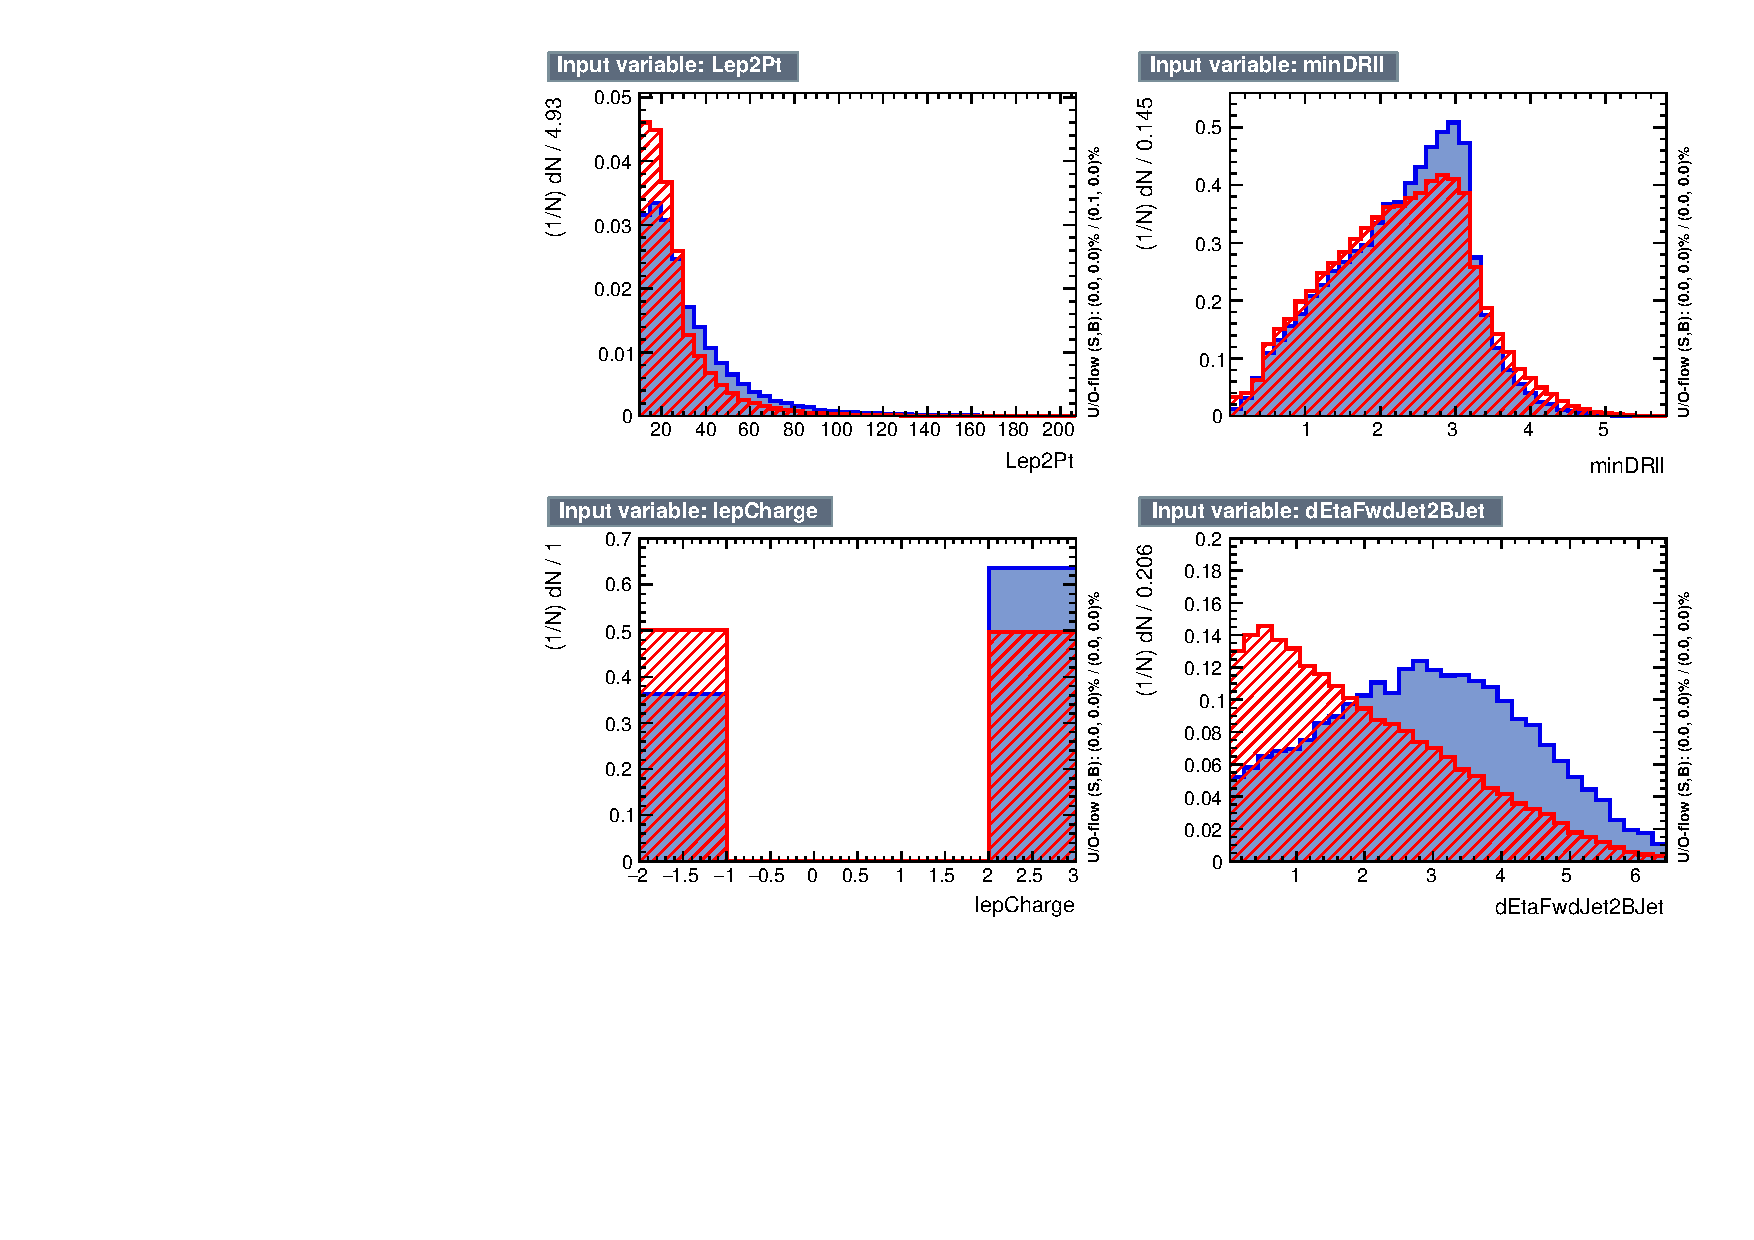
\includegraphics[width=0.66\textwidth]{4var_tt.pdf}
%% \caption{BDT inputs as seen by TMVA (signal, in blue, is \tHq, background, in red, is \ttbar) for the same sign dilepton channel, discriminated against \ttbar\ background.} 
%% \label{mva_input_2lss_tt}
%% \end{figure}

%% \begin{figure} [!h]
%%   \centering
%%   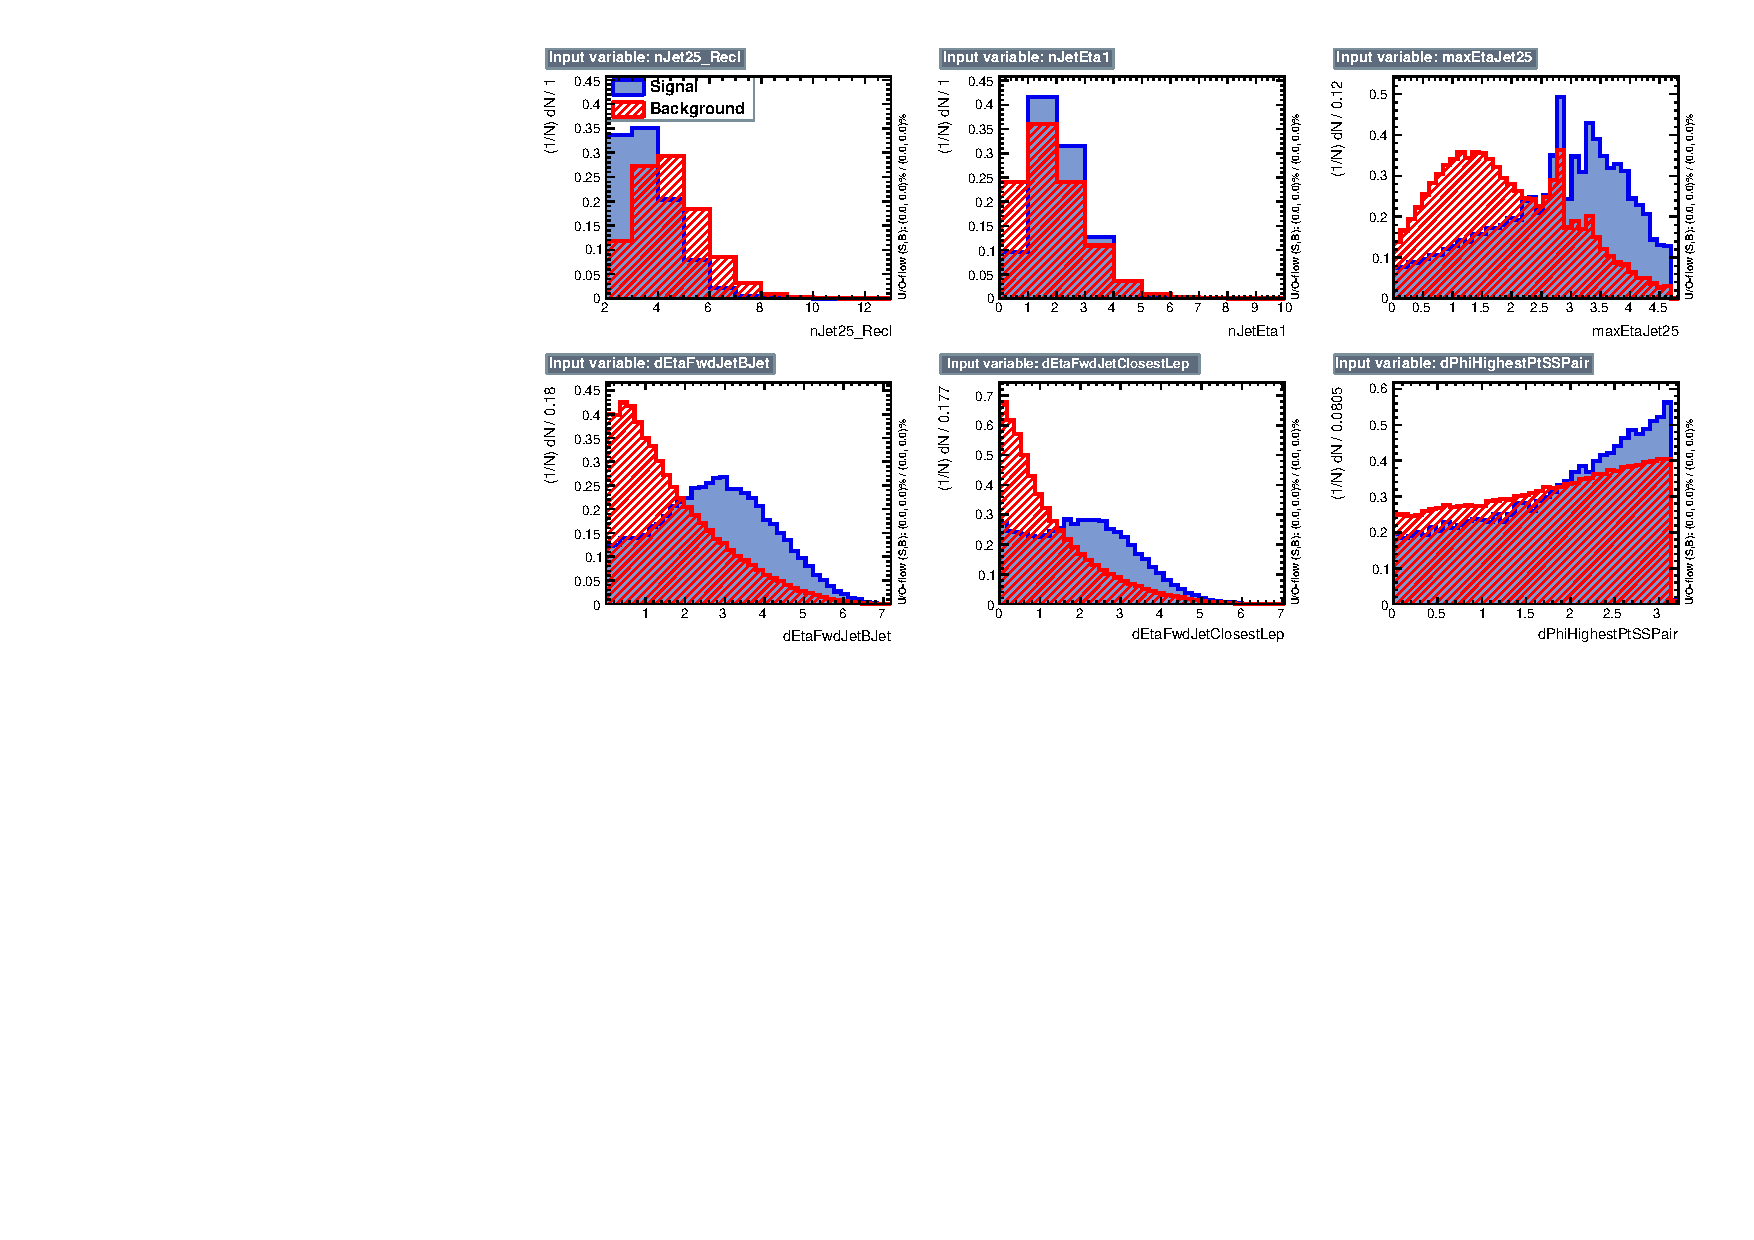
\includegraphics[width=\textwidth]{6var_ttv.pdf}
%%   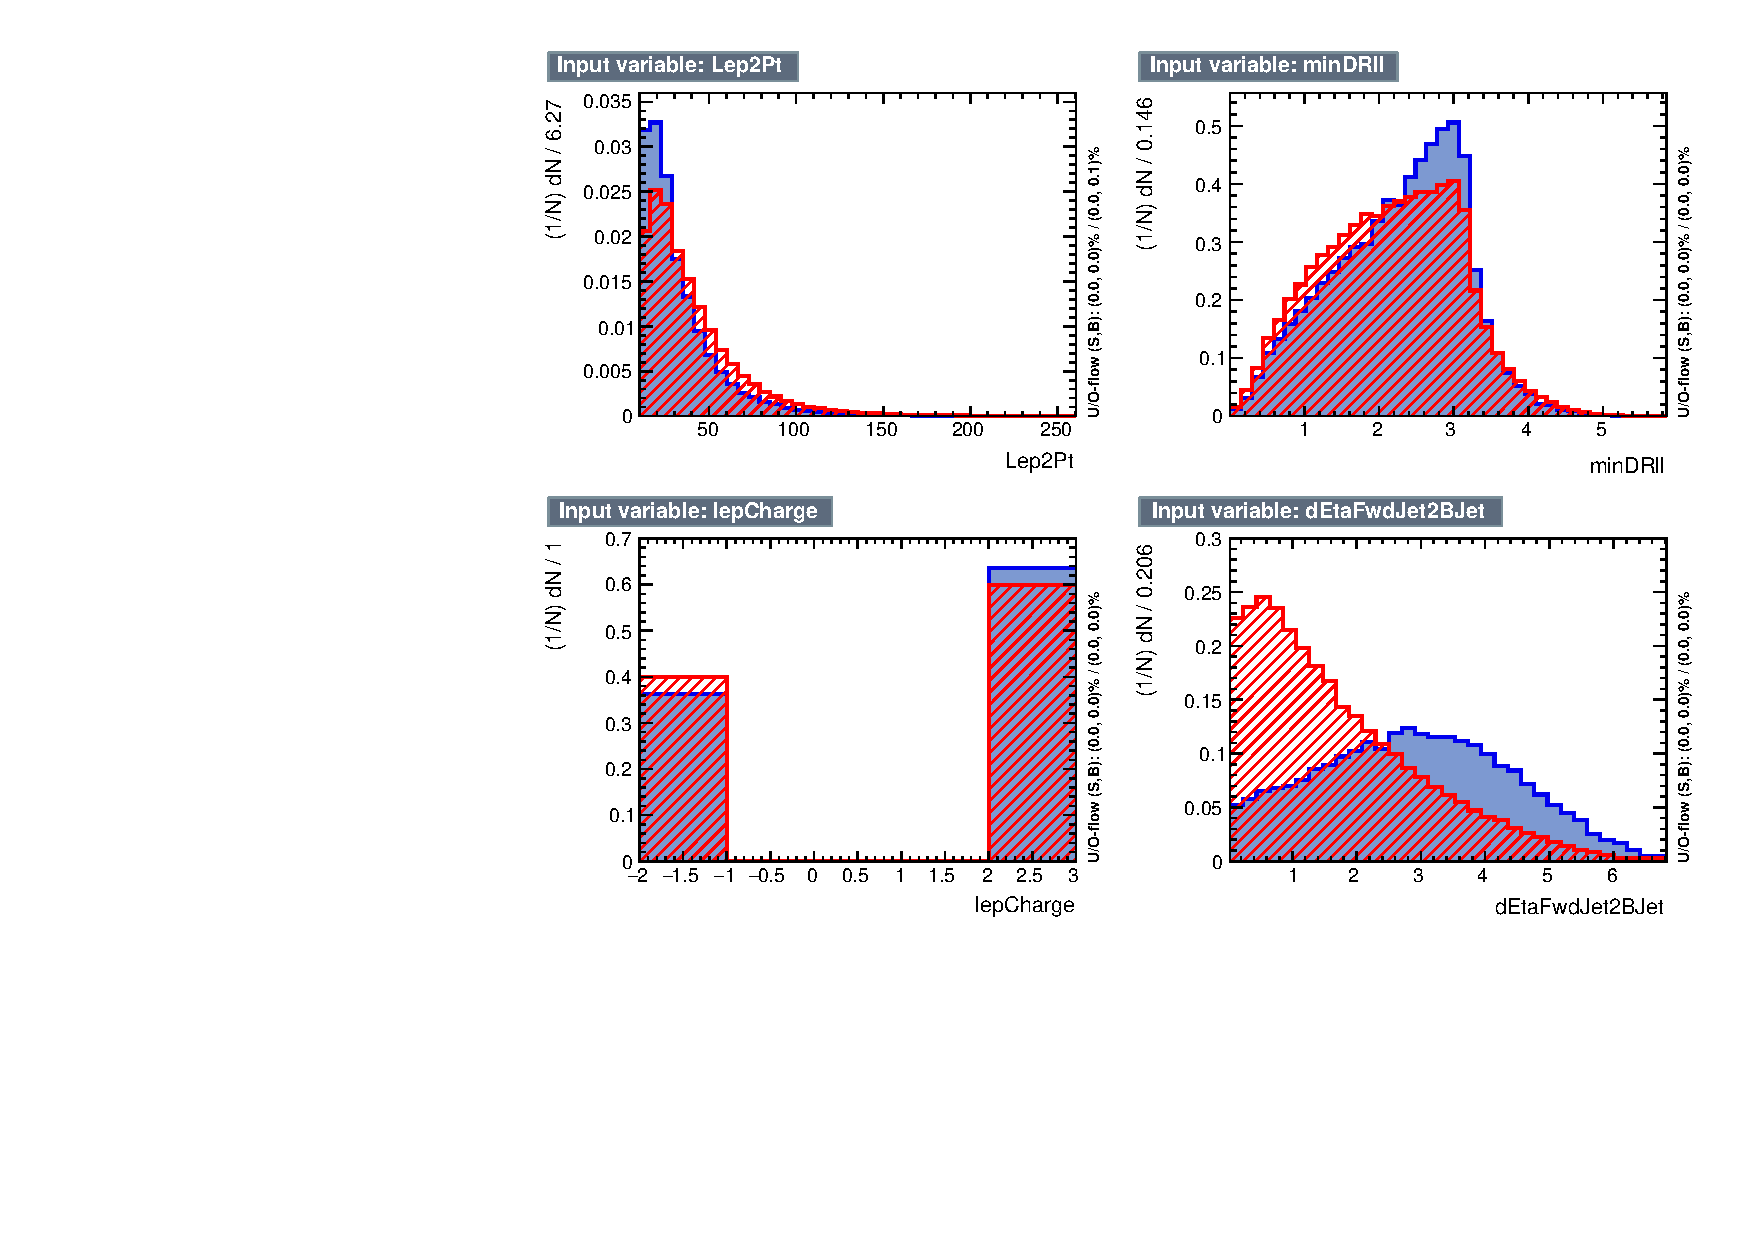
\includegraphics[width=0.66\textwidth]{4var_ttv.pdf}
%% \caption{BDT inputs as seen by TMVA (signal, in blue, is \tHq, background, in red, is \ttW+\ttZ) for the same sign dilepton channel, discriminated against \ttV\ background.}
%% \label{mva_input_2lss_ttv}
%% \end{figure}

Note that splitting the training in two groups reveals that some variables show opposite behavior for the two background sources; potentially screening the discrimination power if they were to be used in a single discriminant. For some other variables the distributions are similar in both background cases.

From table~\ref{tab:bdtinputs}, it is clear that the input variables are correlated to some extend. These correlations play an important role for some MVA methods like the Fisher discriminant method in which the first step consist of performing a linear transformation to an phase space where the correlations between variables are removed. In case a boosted decision tree (BDT) method however, correlations do not affect the performance. Figure~\ref{mva_corr} show the linear correlation coefficients for signal and background for the two training cases (the signal values are identical by construction). As expected, strong correlations appears for variables related to the forward jet activity. Same trend is seen in case of the same sign dilepton channel in Figure~\ref{mva_corr_2lss}.

\begin{figure} [!h]
  \centering
   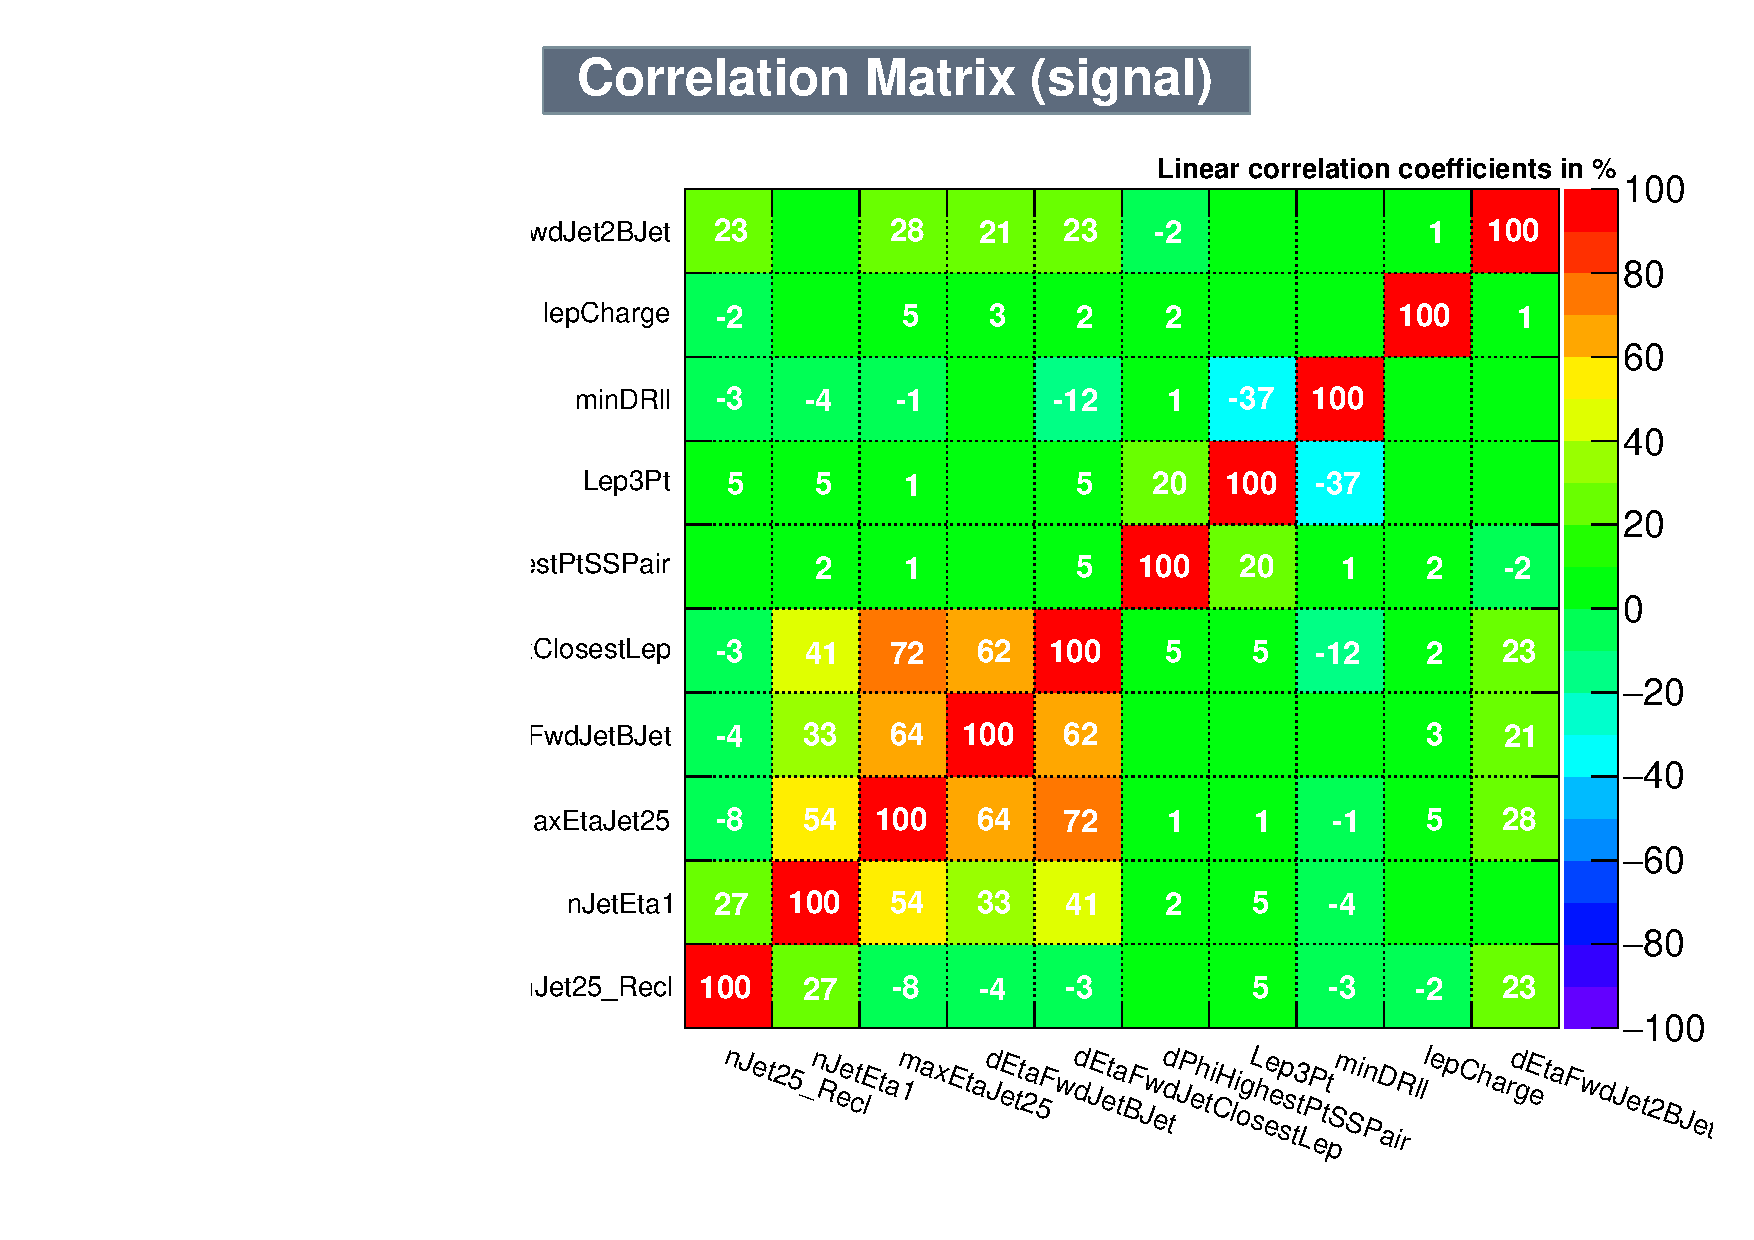
\includegraphics[width=0.32\textwidth]{corr_signal.pdf}
   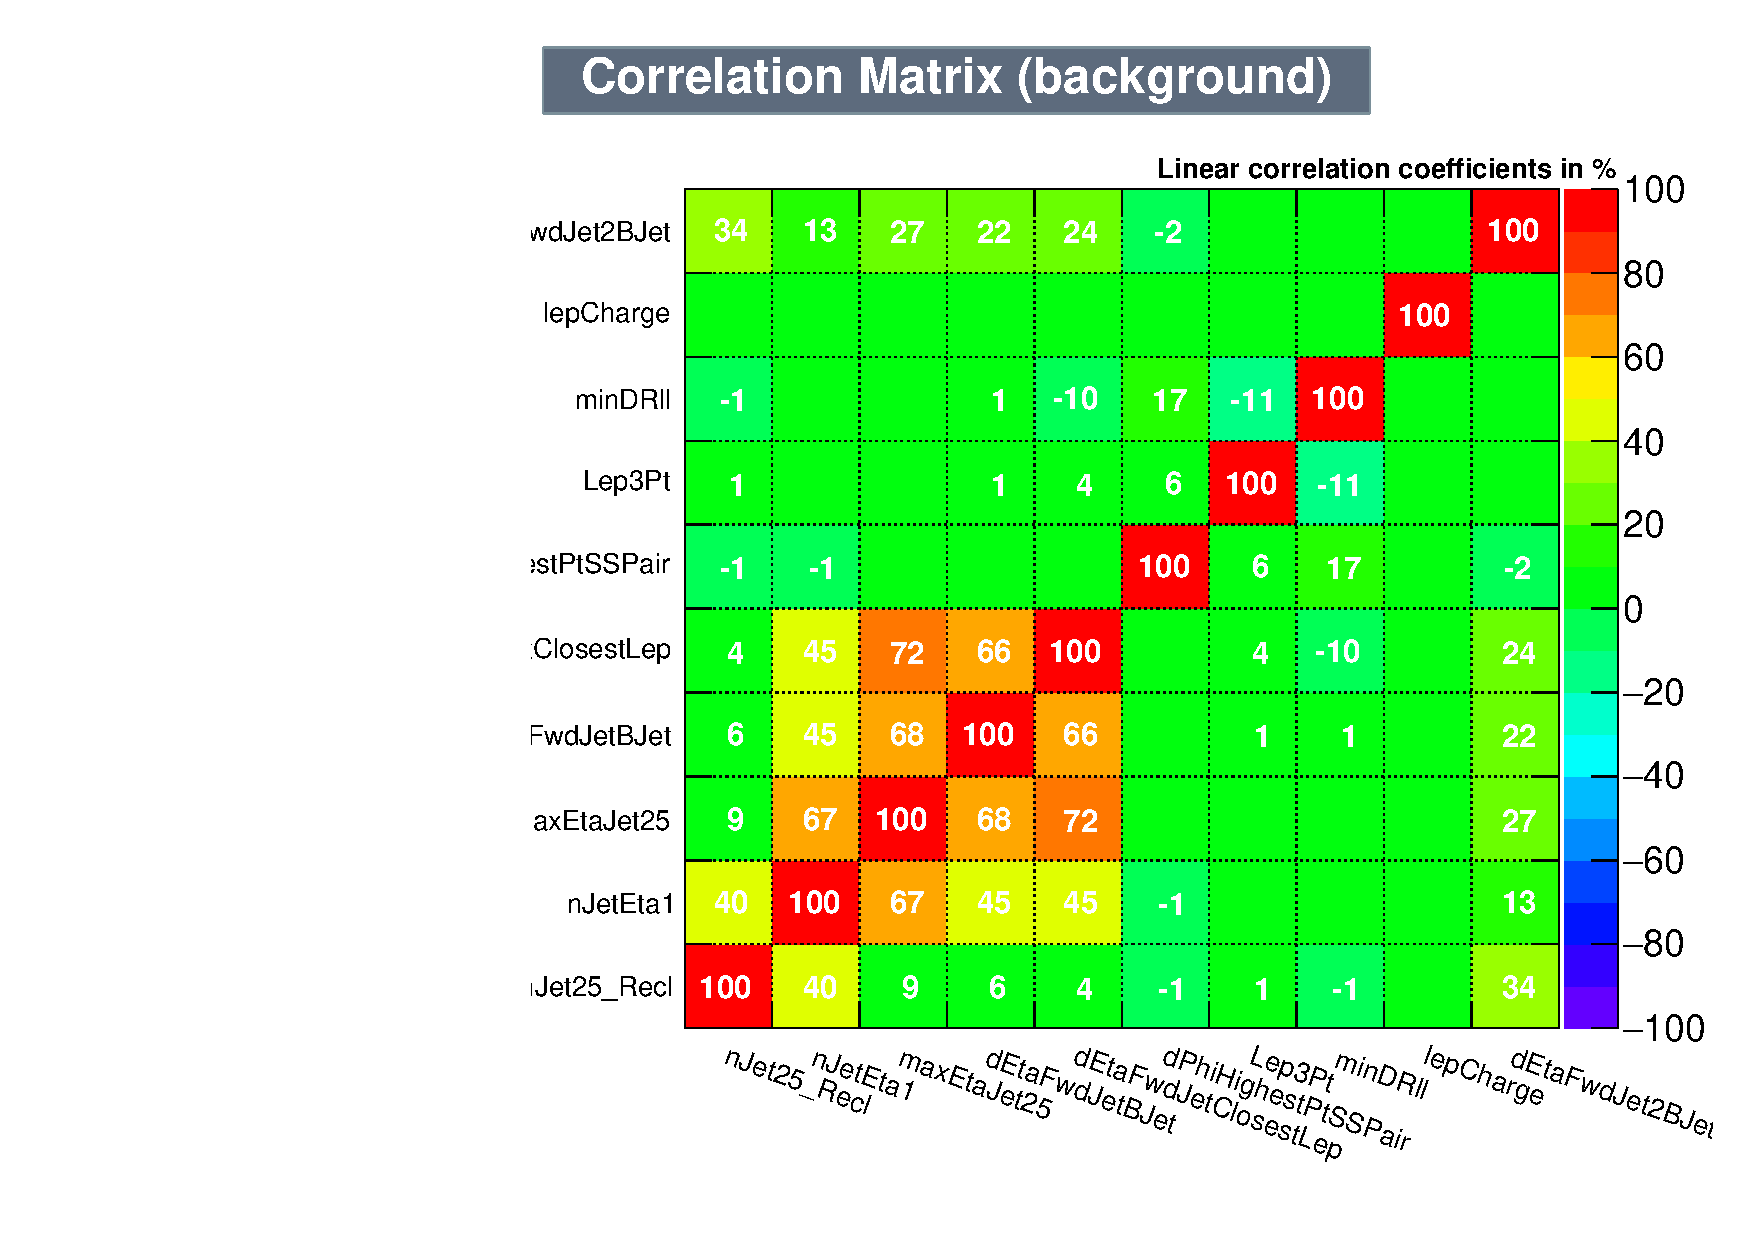
\includegraphics[width=0.32\textwidth]{corr_tt.pdf}
   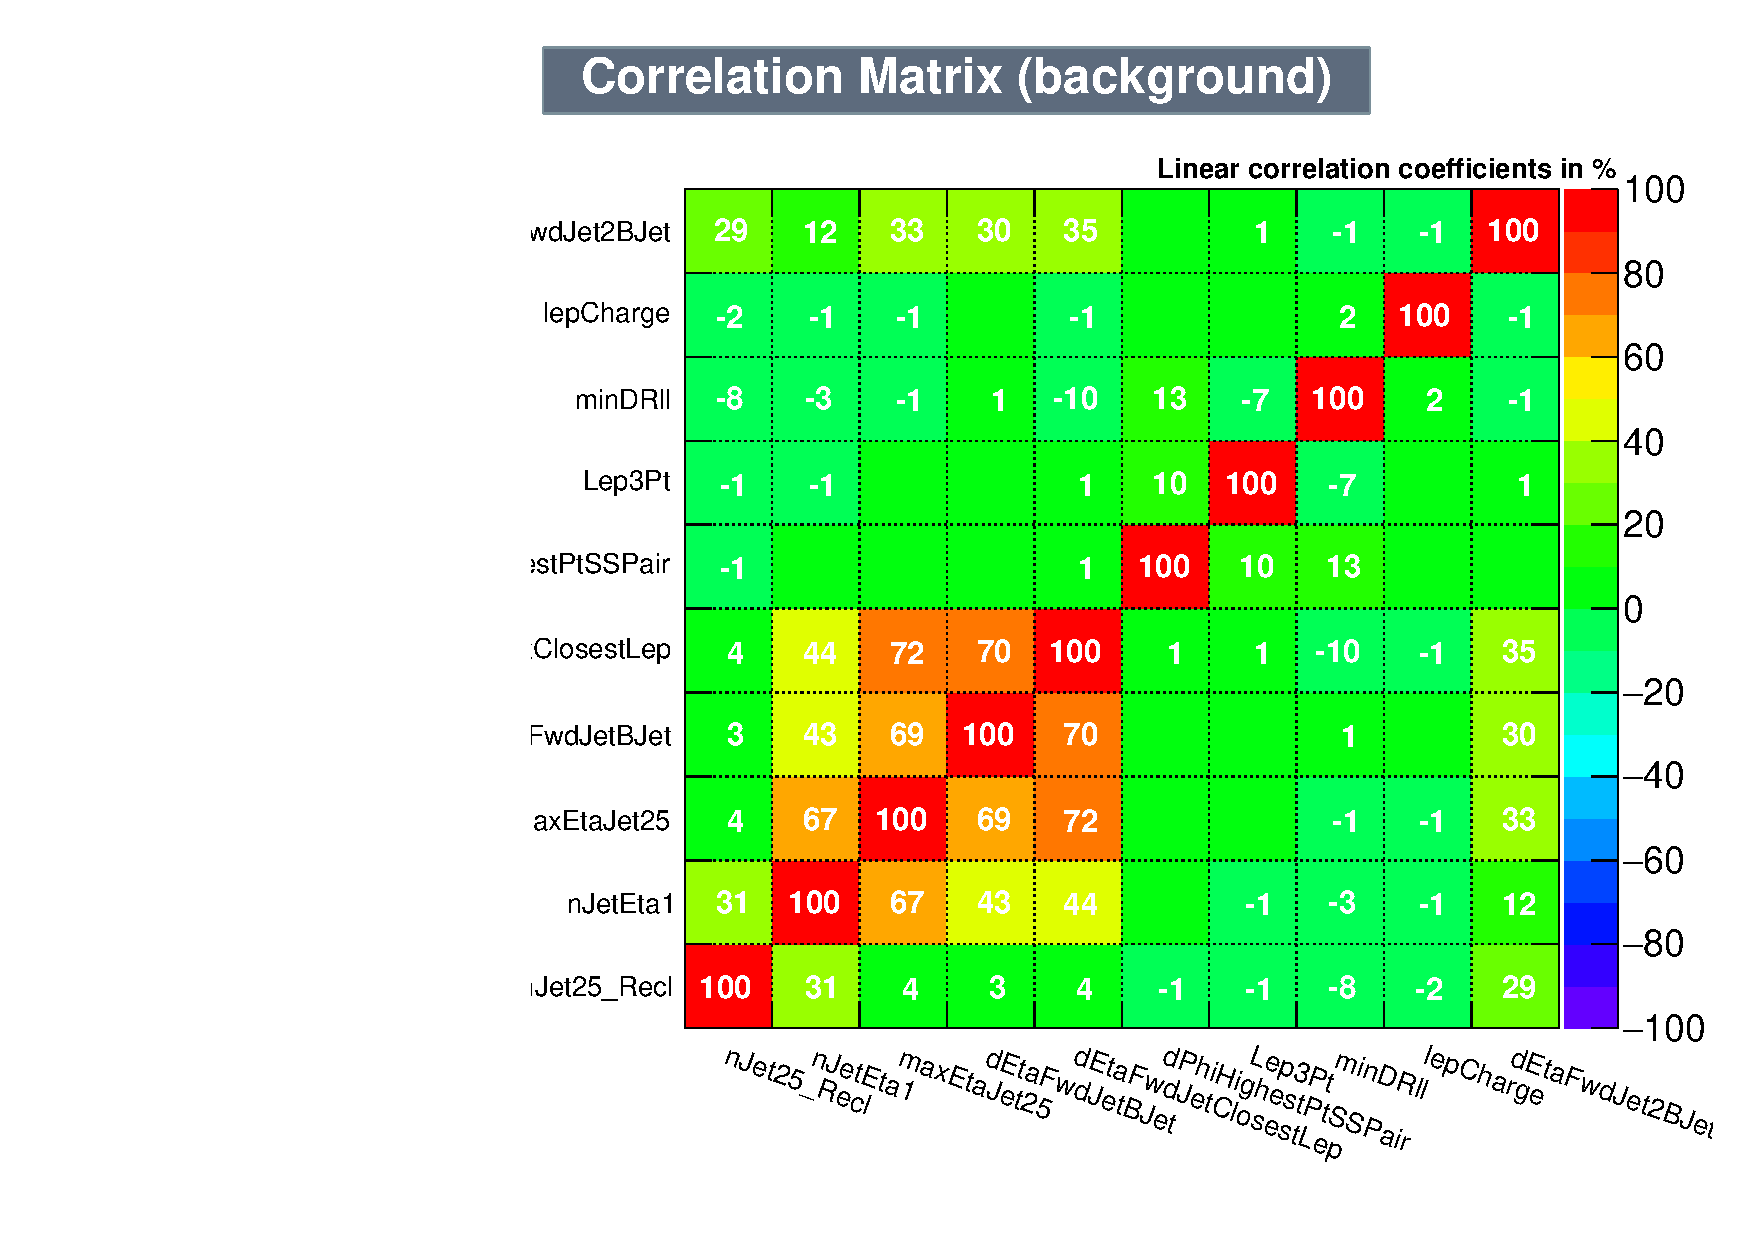
\includegraphics[width=0.32\textwidth]{corr_ttv.pdf}

\caption[Correlation matrices for the input variables in the TMVA.]{ Signal (left), \ttbar\ background (middle), and \ttV\ background (right.) correlation matrices for the input variables in the TMVA analysis for the three lepton channel.}
\label{mva_corr}
\end{figure}

%% \begin{figure} [!h]
%%   \centering
%%   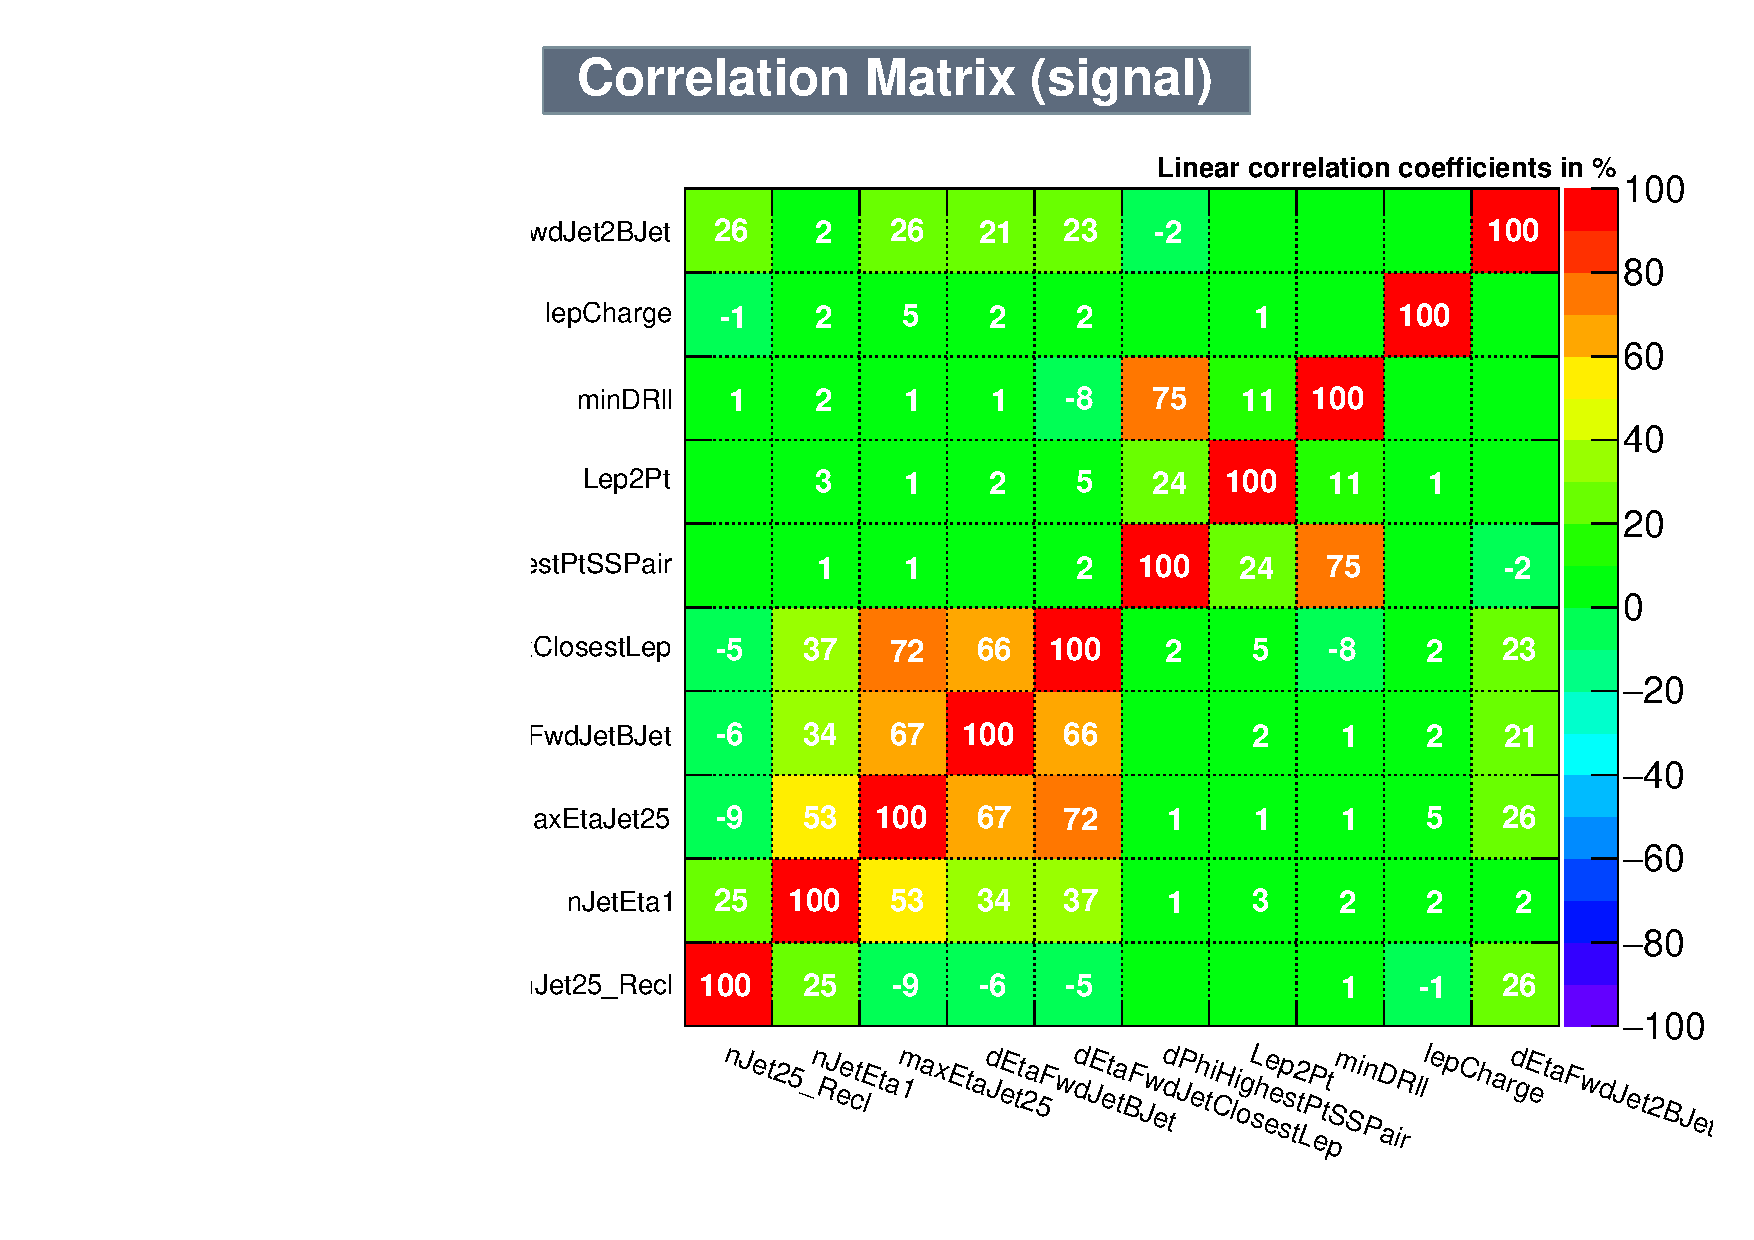
\includegraphics[width=0.32\textwidth]{sig_corr_tt_2lss.pdf}
%%   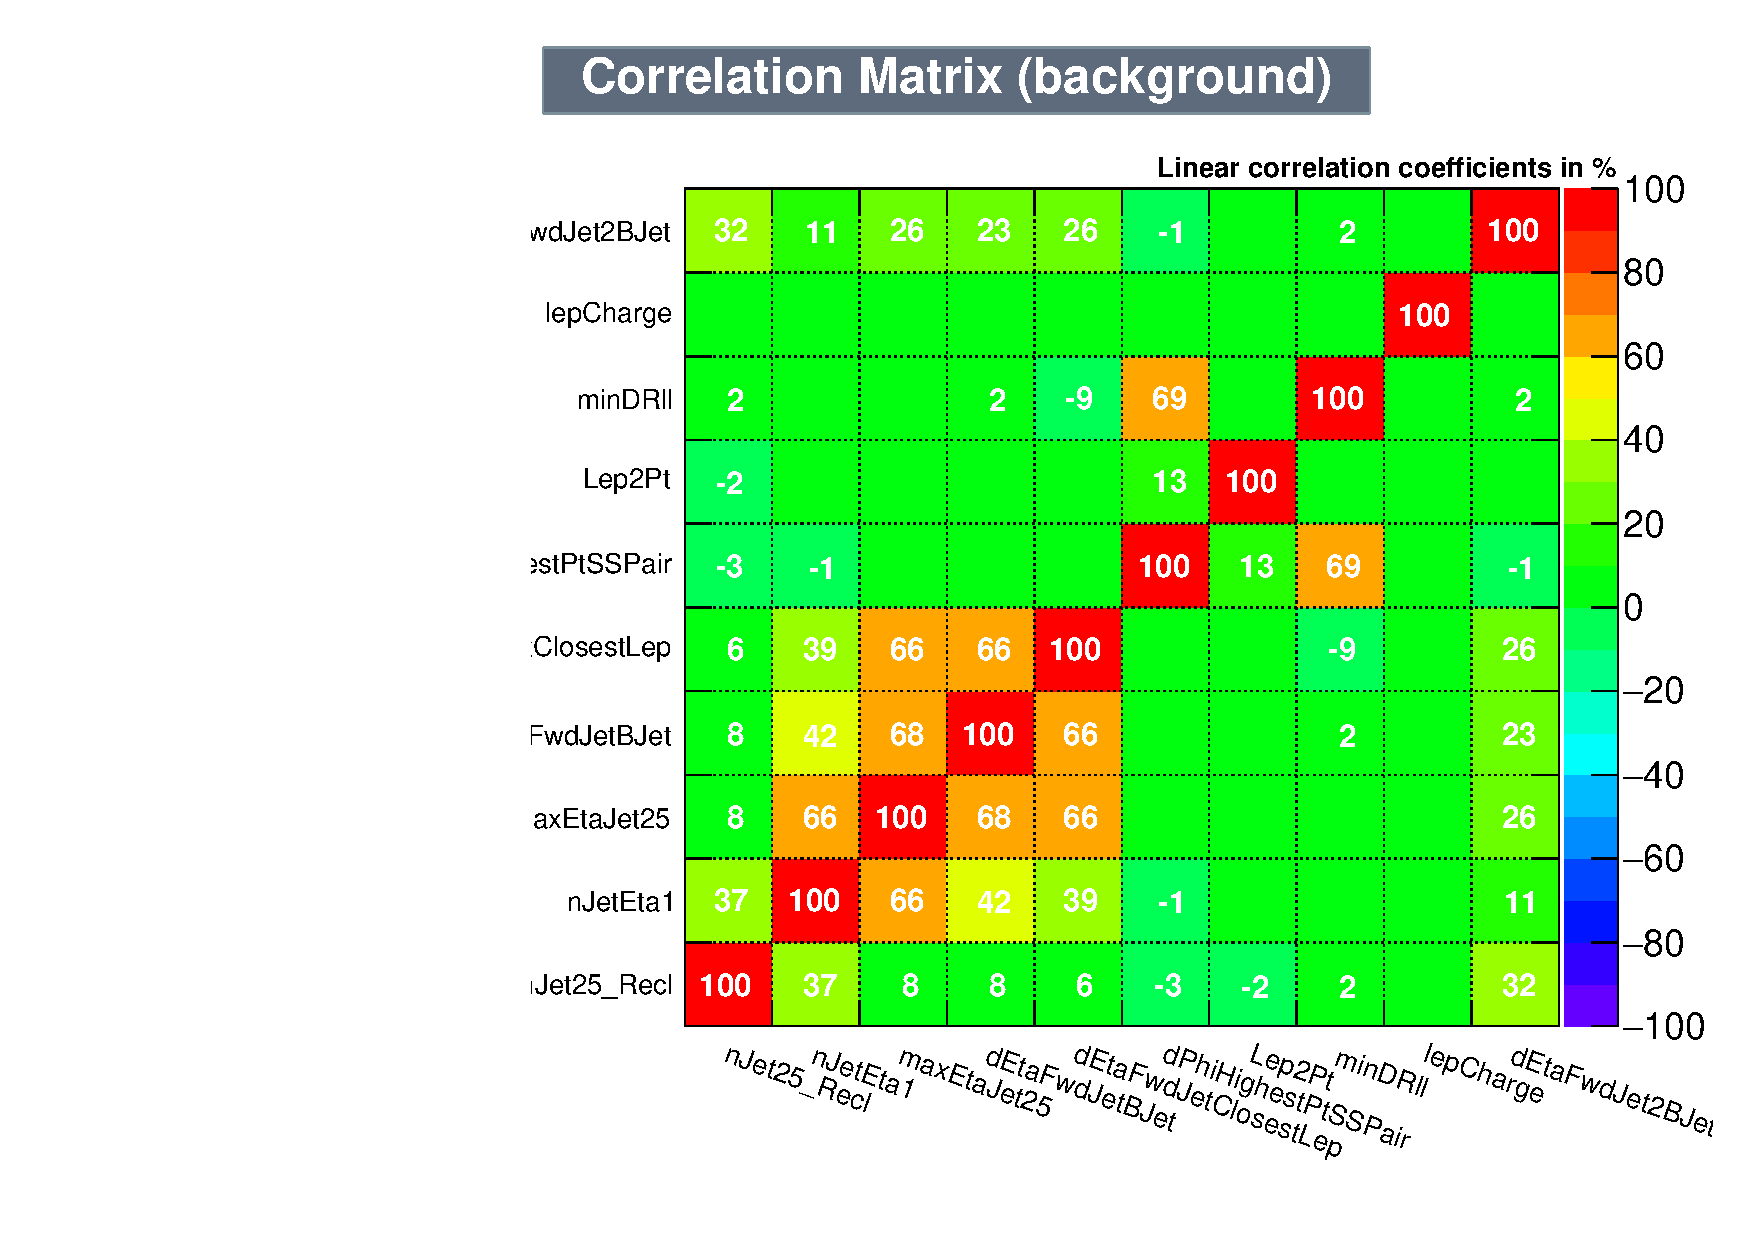
\includegraphics[width=0.32\textwidth]{bkg_corr_tt_2lss.pdf}
%%   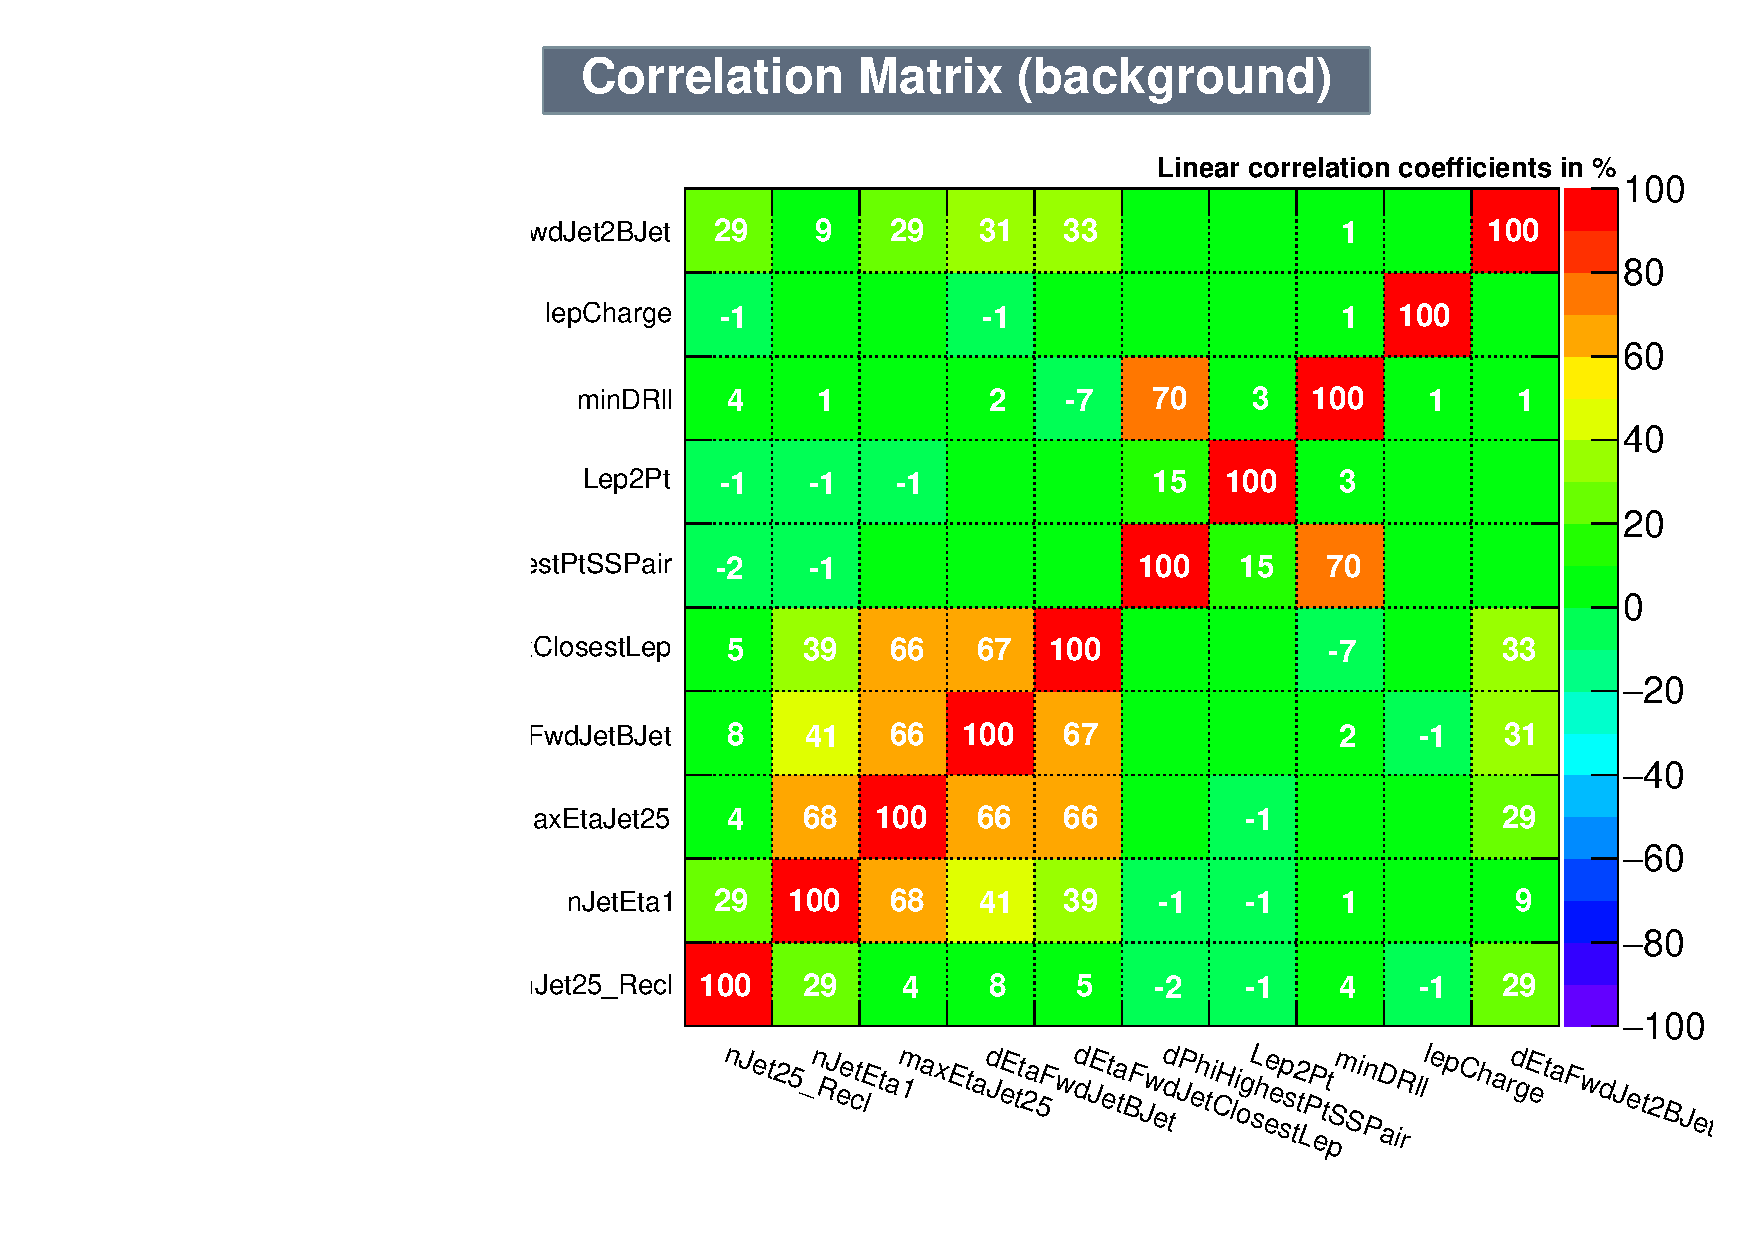
\includegraphics[width=0.32\textwidth]{bkg_corr_ttv_2lss.pdf}
%% \caption{Signal and Background correlation matrices for the input variables in the TMVA analysis for the same sign dilepton channel, for the signal (left), \ttbar\ background (middle), and \ttV\ background (right.)}
%% \label{mva_corr_2lss}
%% \end{figure}

\subsection{Classifiers response}
Several MVA algorithms were evaluated to determine the most appropriate method for this analysis. The plots in Fig.~\ref{roc} (top) show the background rejection as a function of the signal efficiency for \ttbar\ and \ttV\ trainings (ROC curves) for the different algorithms that were evaluated.

\begin{figure} [!h]
  \centering
   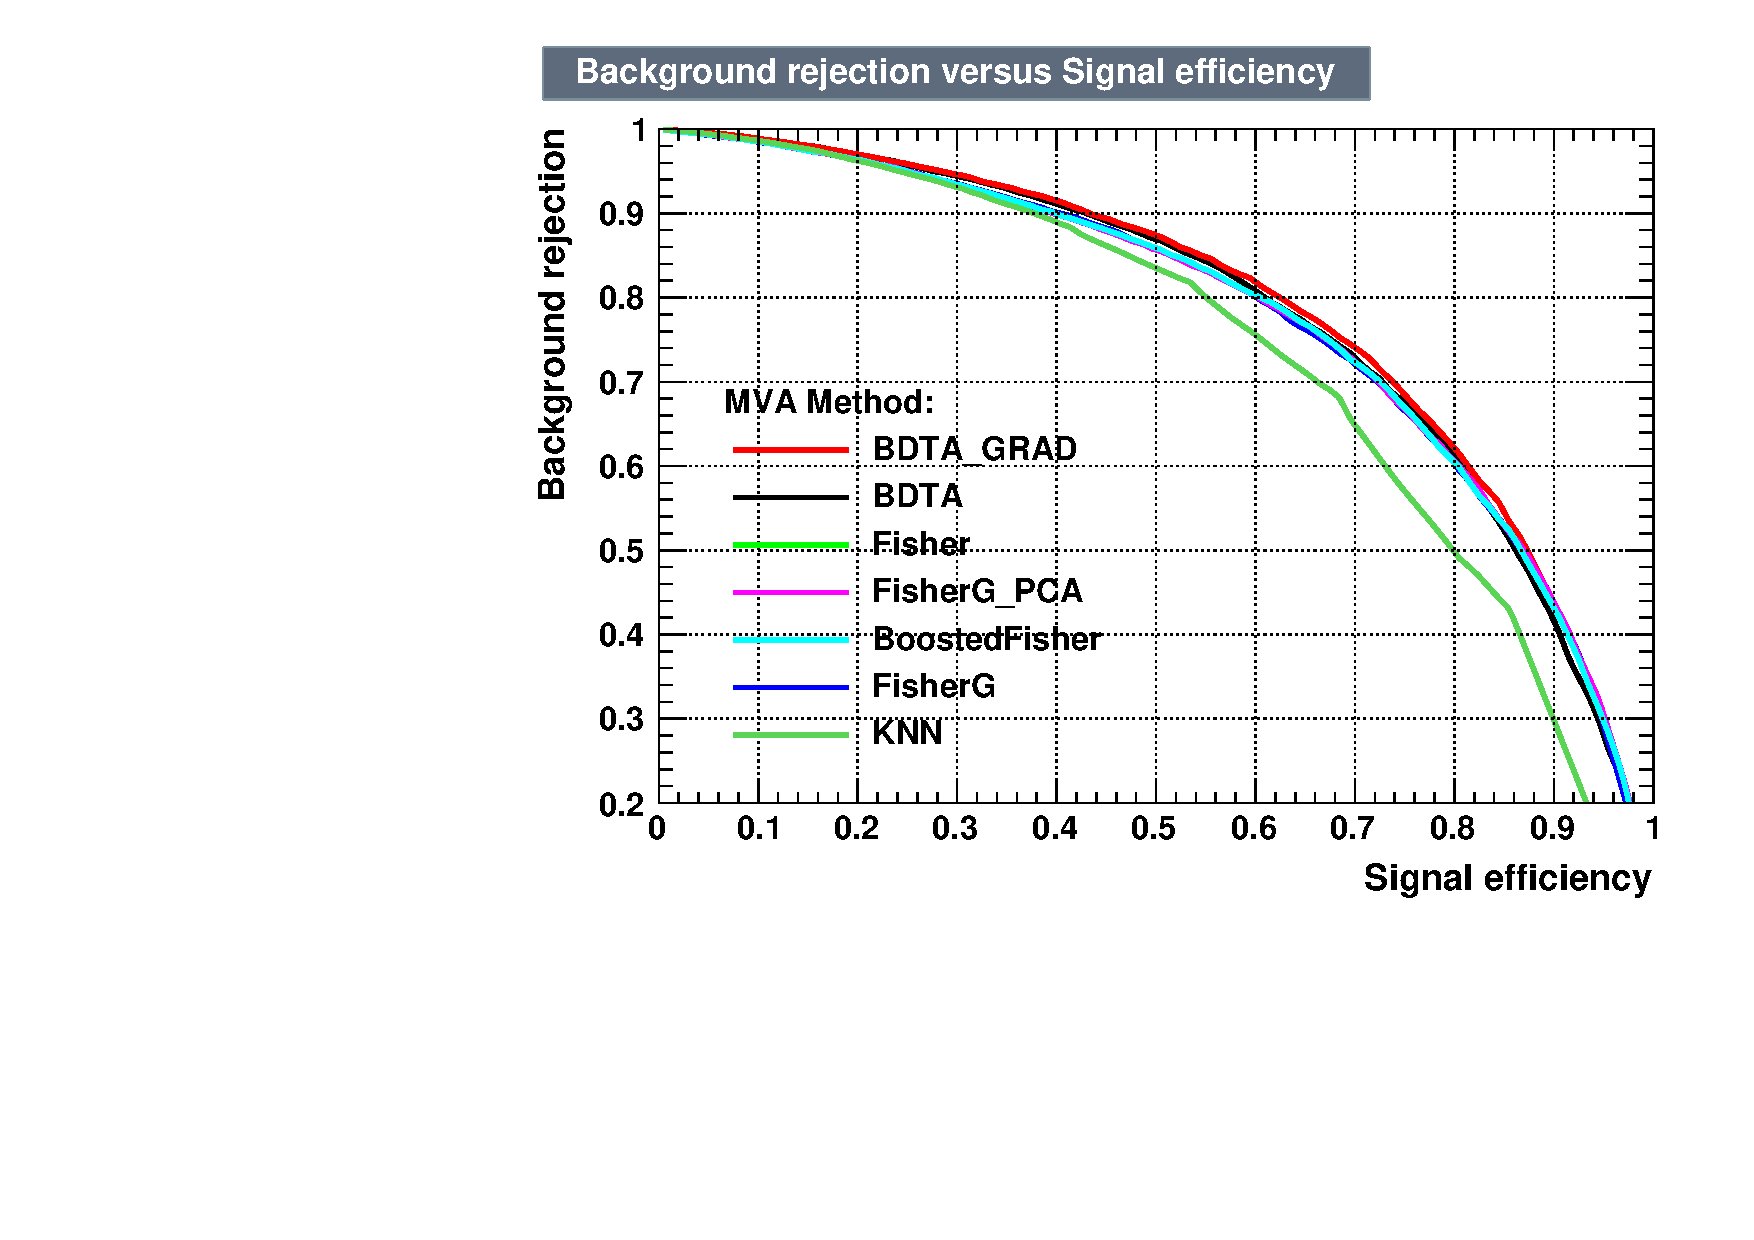
\includegraphics[width=0.4\textwidth]{roc_ttv_3l_multimva.pdf}
   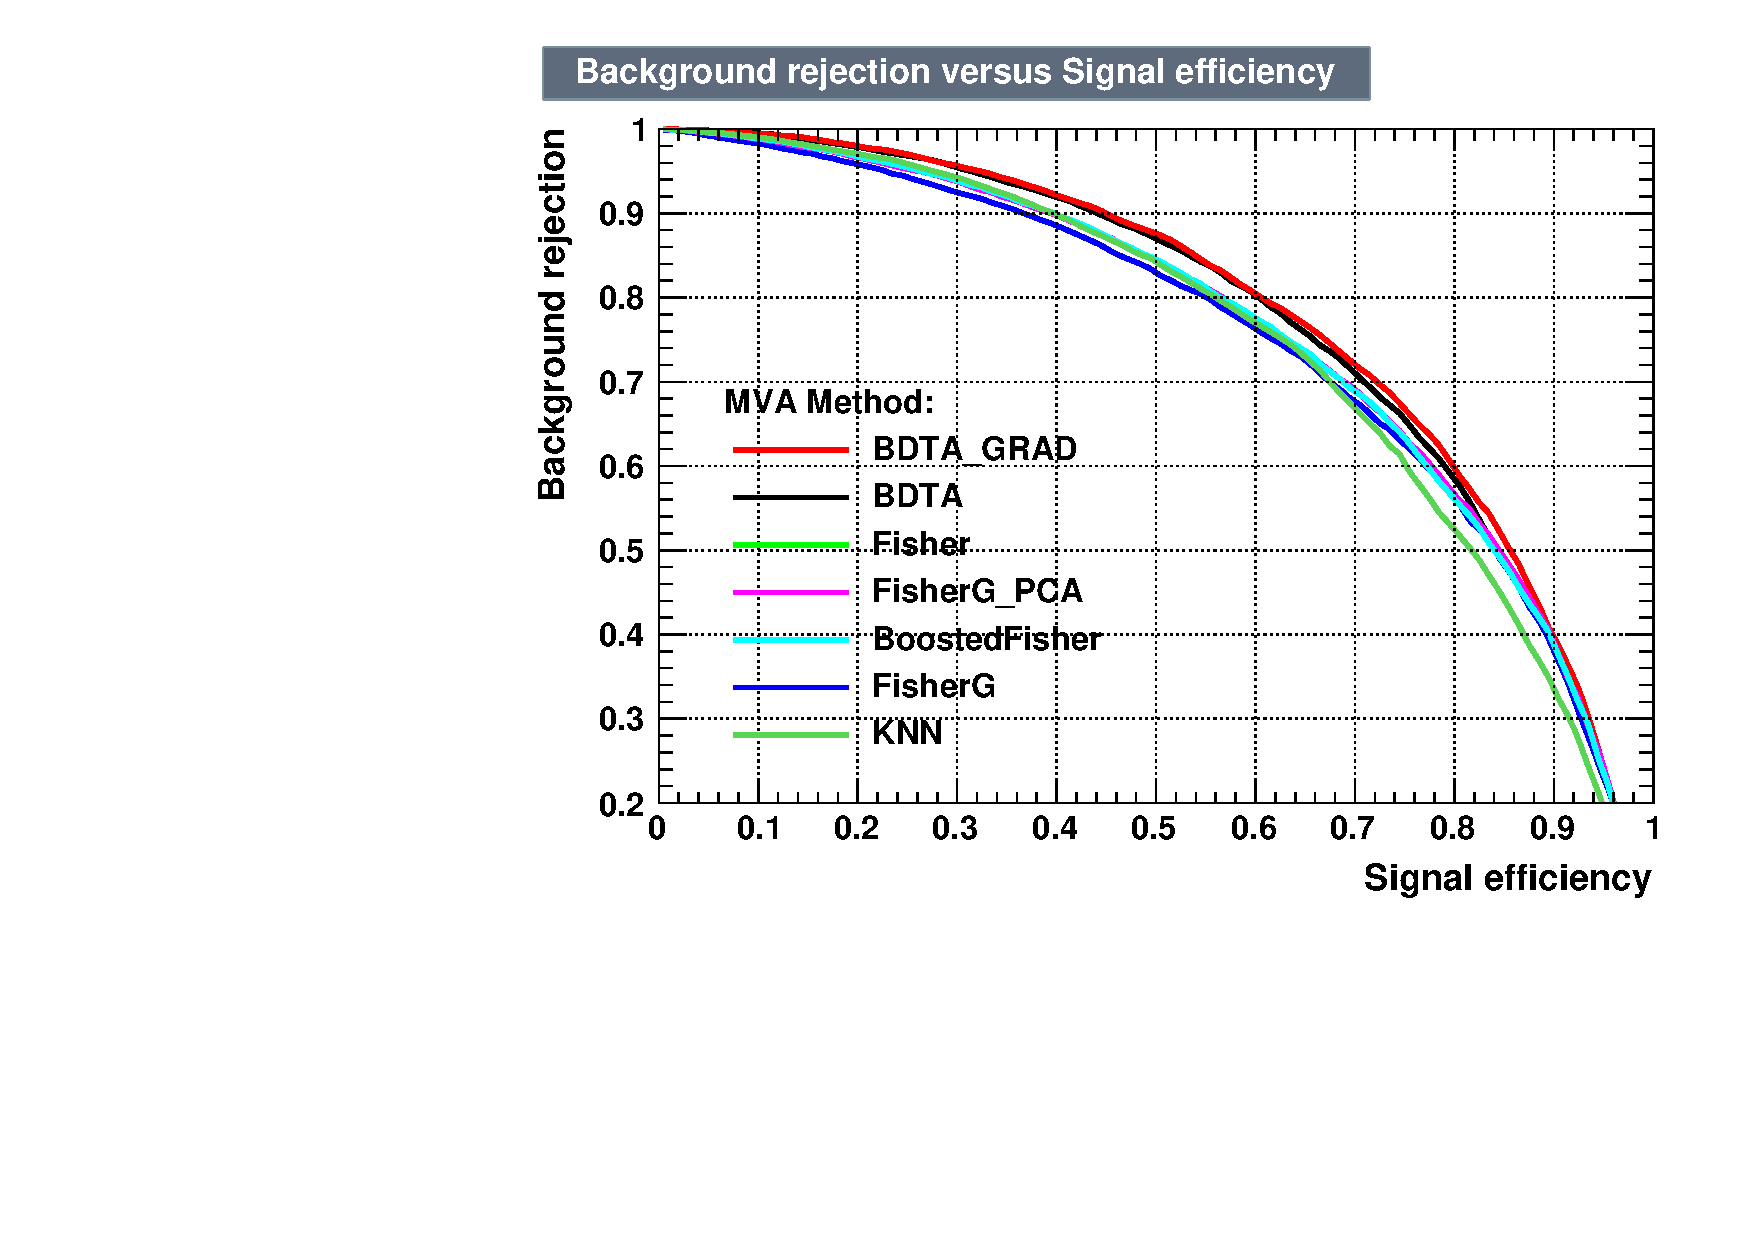
\includegraphics[width=0.4\textwidth]{roc_tt_3l_multimva.pdf} \\
   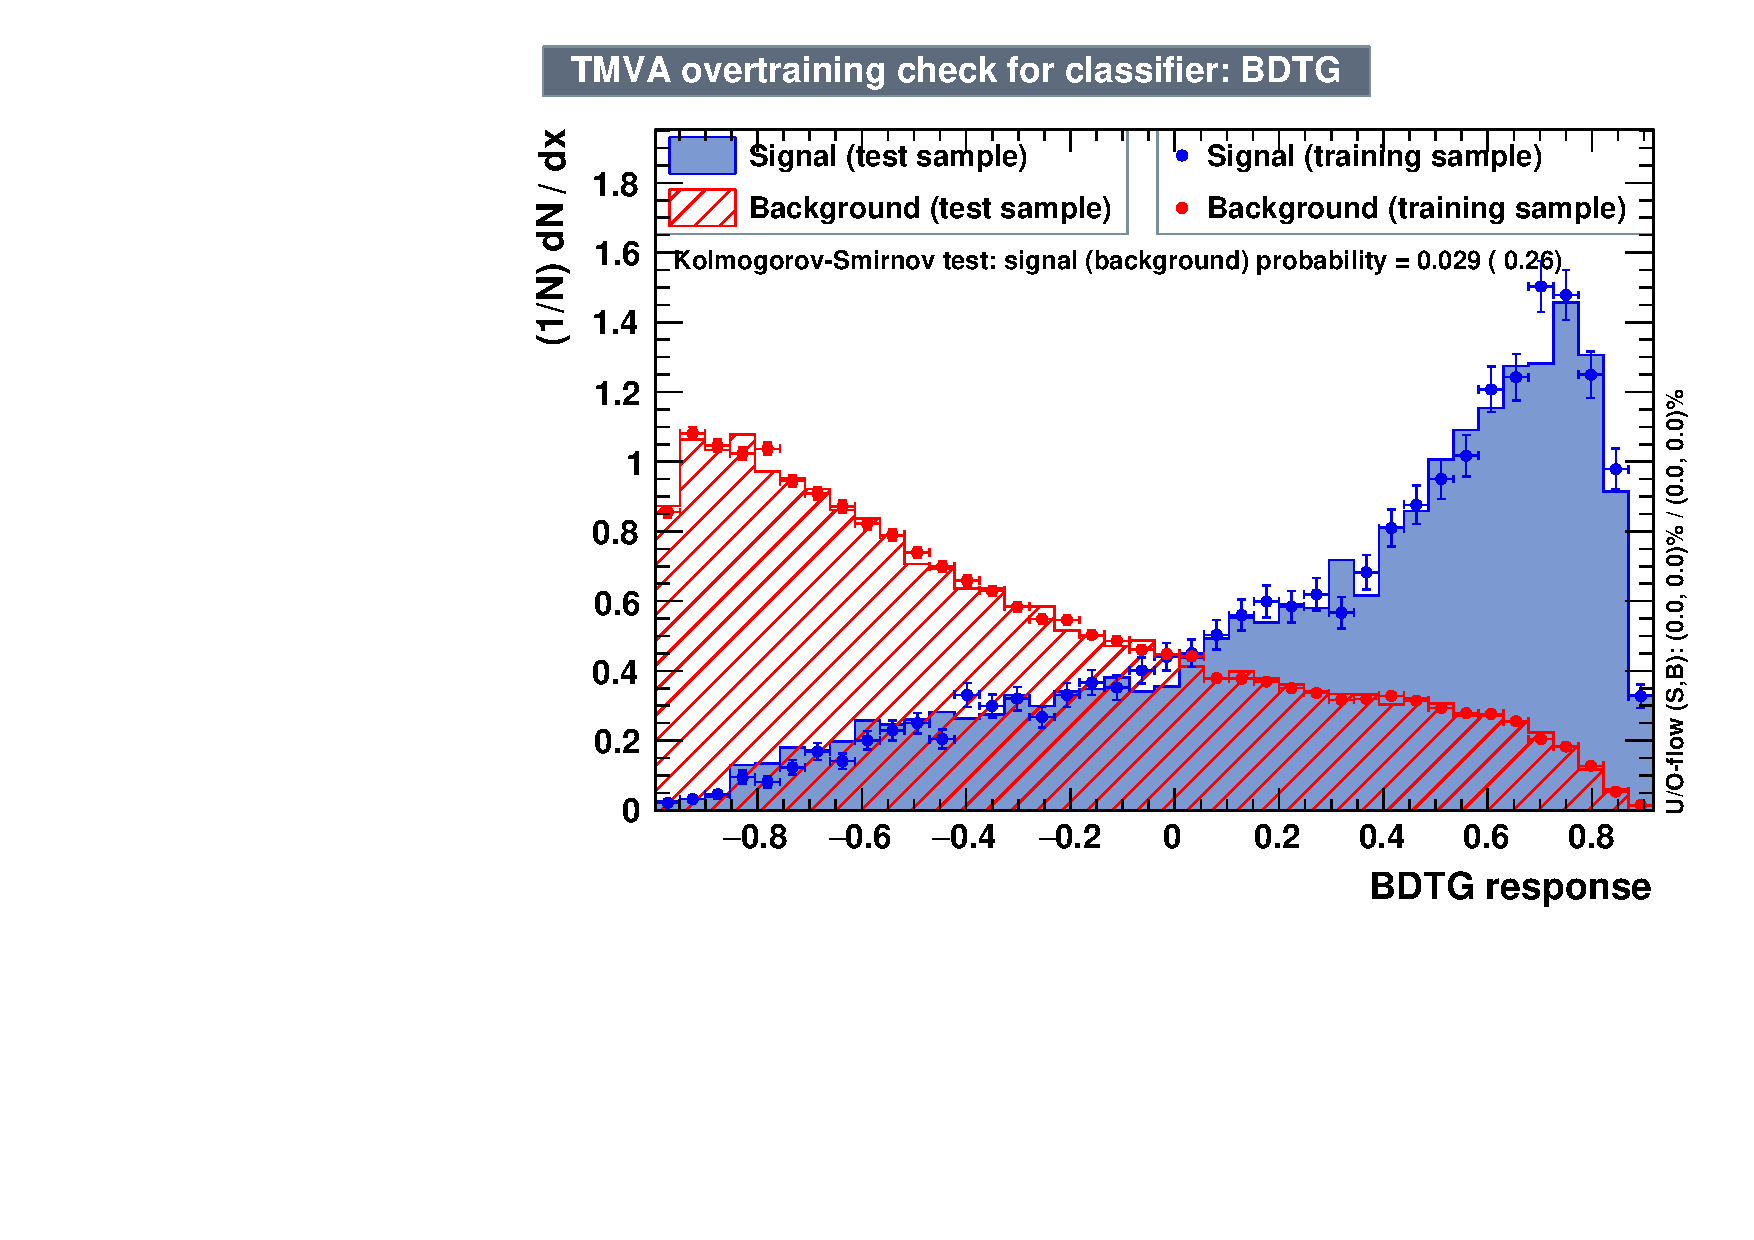
\includegraphics[width=0.4\textwidth]{bdt_response_ttv_3l.pdf}
   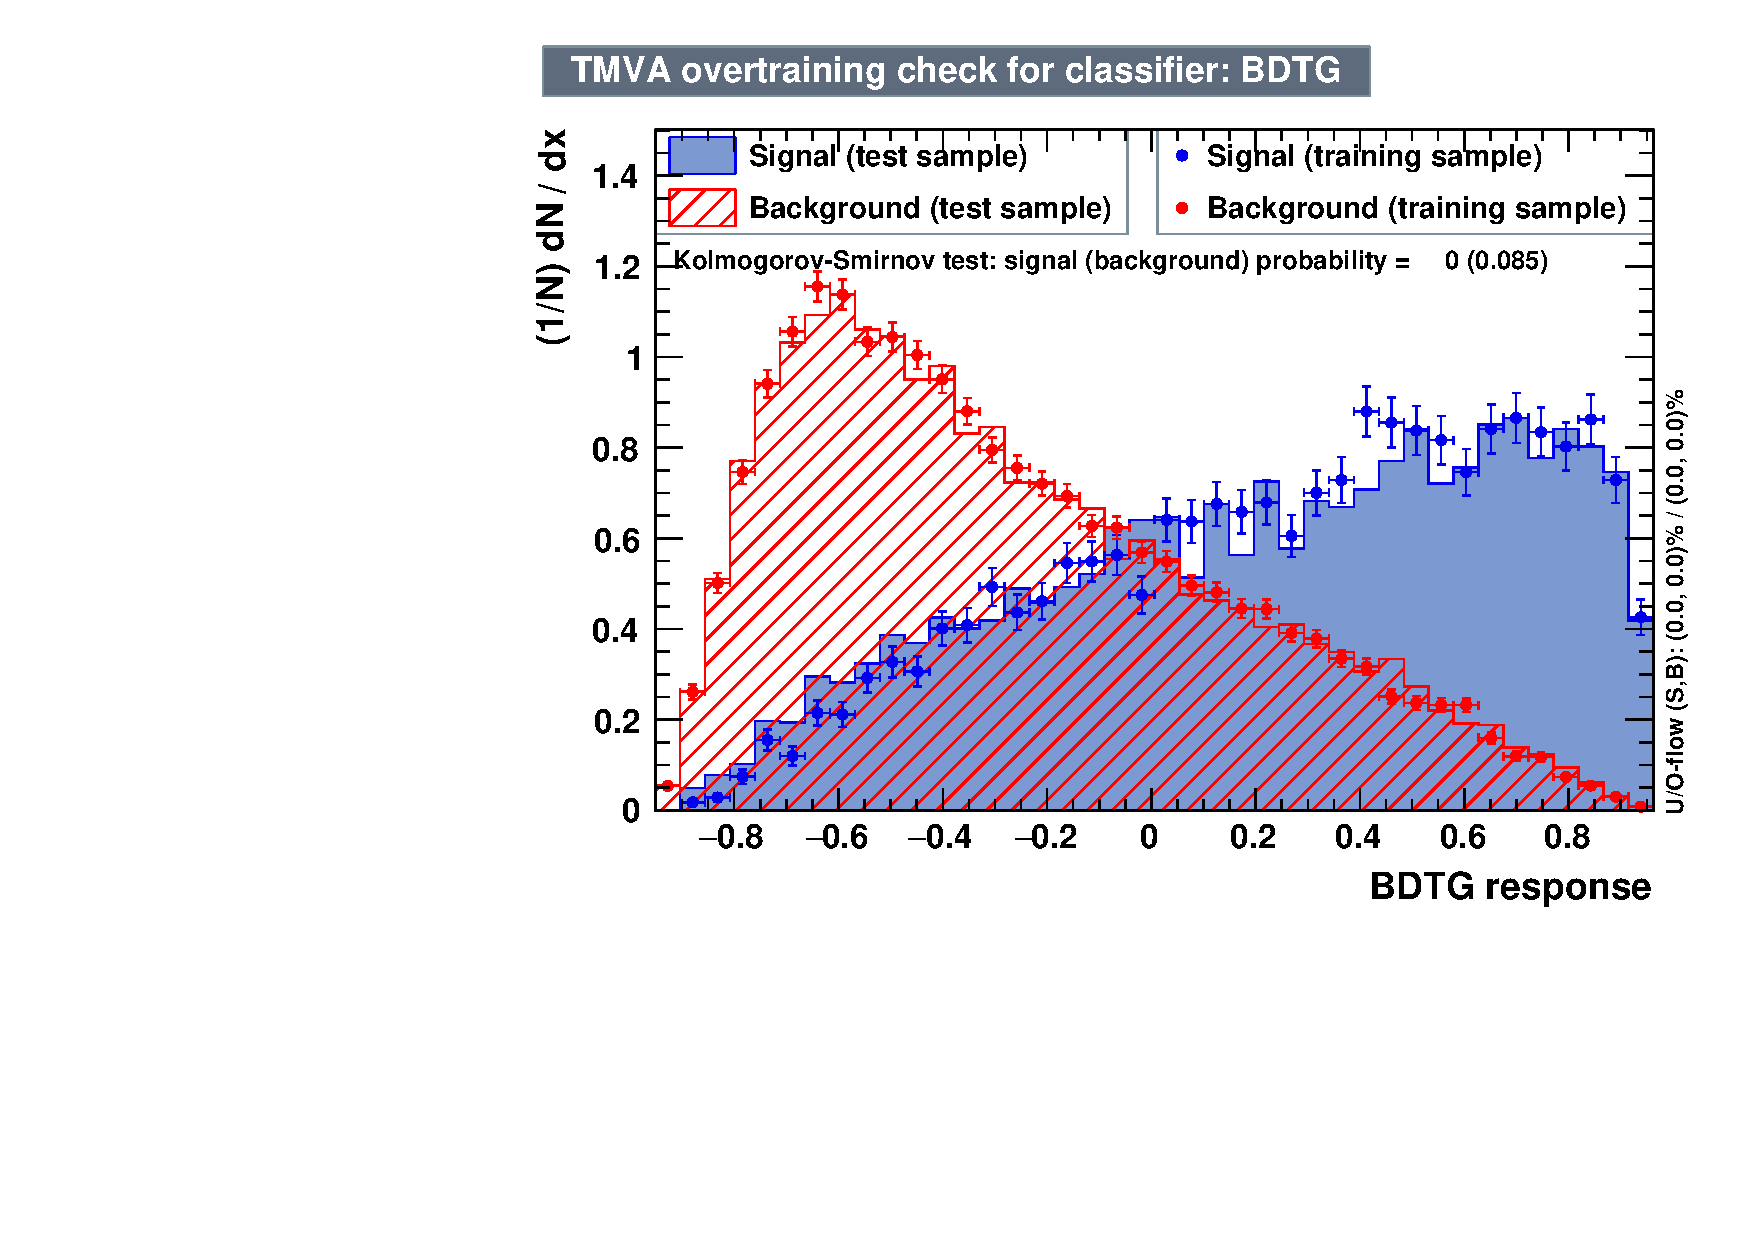
\includegraphics[width=0.4\textwidth]{bdt_response_tt_3l.pdf}
\caption[MVA classifiers performance.]{Top: background rejection vs signal efficiency (ROC curves) for various MVA classifiers (top) in the three lepton channel against \ttV\ (left) and \ttbar\ (right). Bottom: classifier output distributions for the gradient boosted decision trees, for training against \ttV\ (left) and against \ttbar\ (right).}
\label{roc}
\end{figure} 

%% \begin{figure} [!h]
%%   \centering
%%    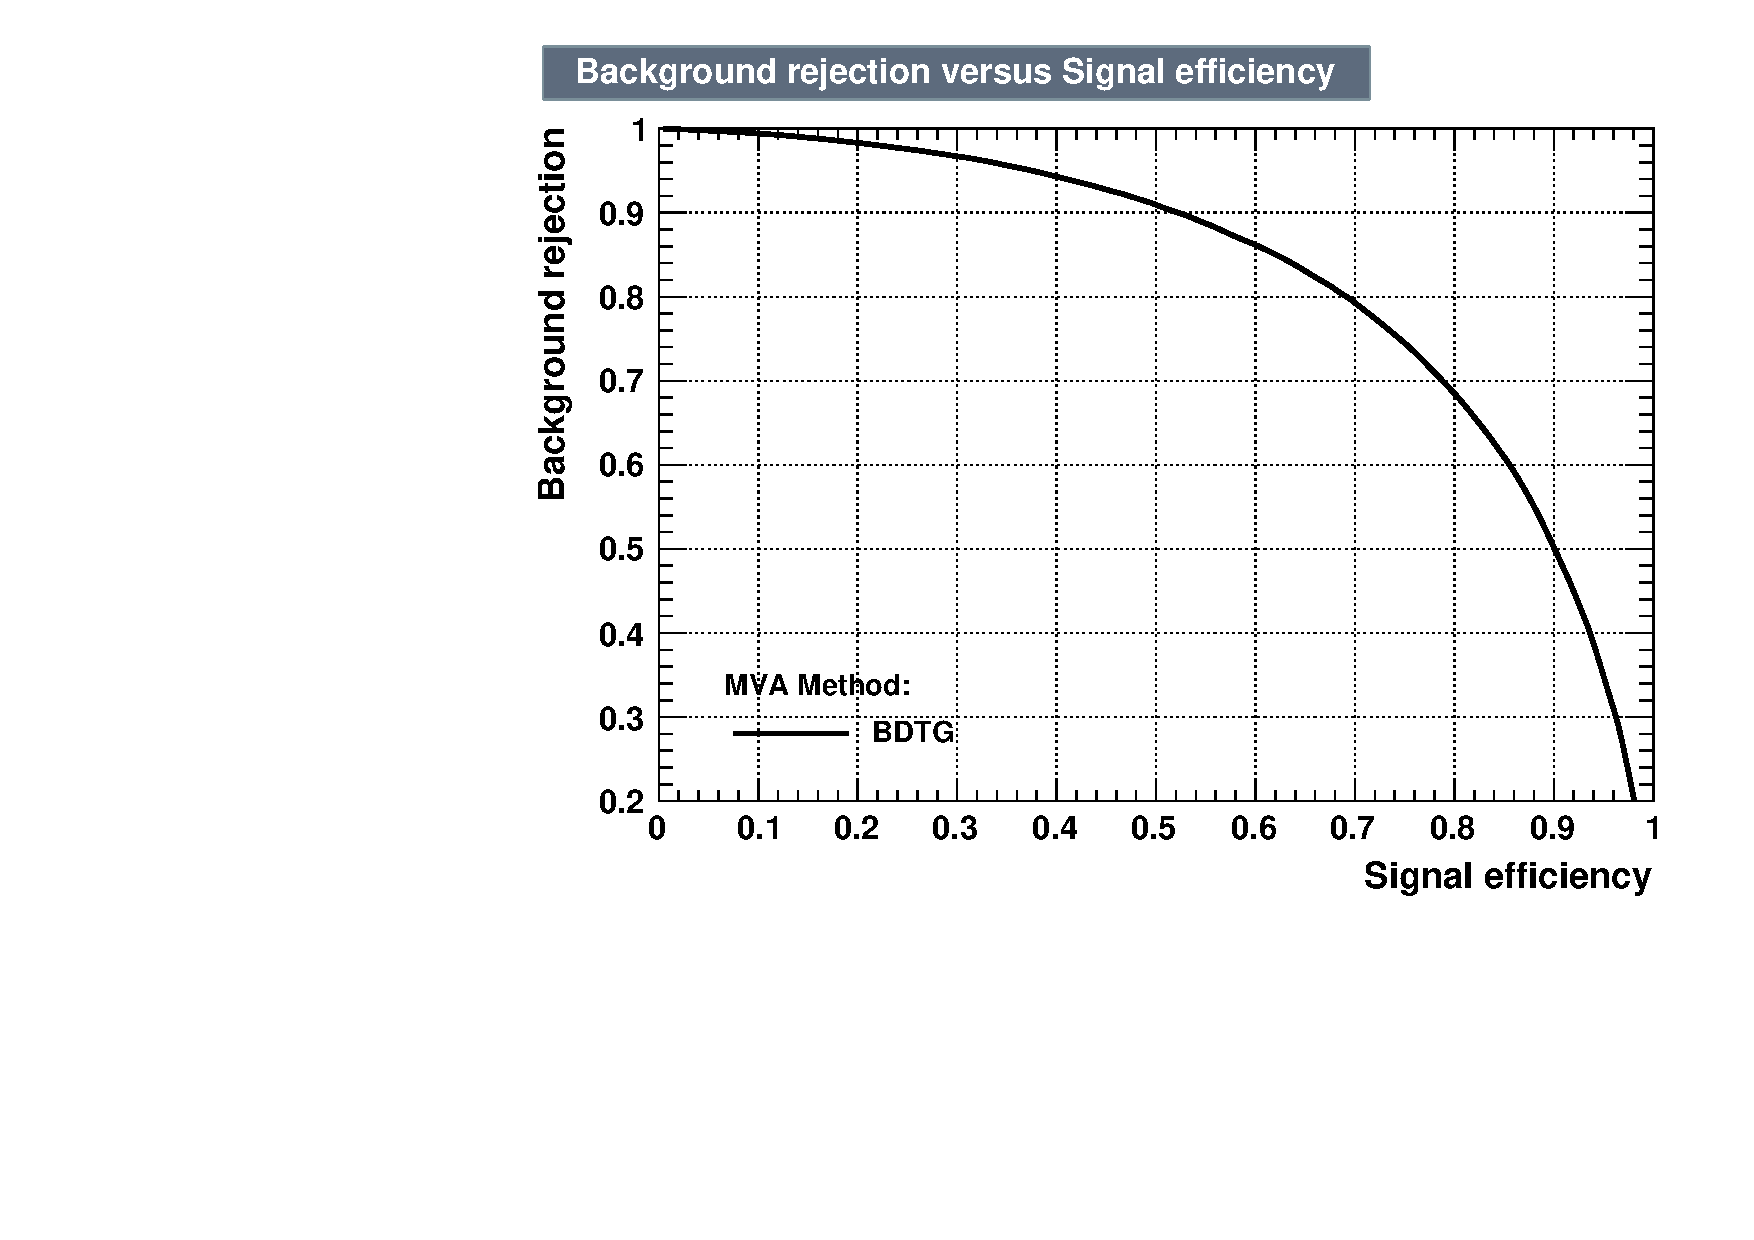
\includegraphics[width=0.4\textwidth]{roc_ttv_2lss.pdf}
%%    \includegraphics[width=0.4\textwidth]{roc_tt_2lss.pdf} \\
%%    \includegraphics[width=0.4\textwidth]{bdt_output_ttv_2lss.pdf}
%%    \includegraphics[width=0.4\textwidth]{bdt_output_tt_2lss.pdf}
%% \caption{Top: background rejection vs signal efficiency (ROC curve) in the same sign dilepton channel for a single discriminator: BDTG, against \ttV\ (left) and \ttbar\ (right). Bottom: classifier output distribution, for training against \ttV\ (left) and against \ttbar\ (right).}
%% \label{output_2lss}
%% \end{figure}

In both cases the gradient boosted decision tree (``BDTA\_GRAD'') classifier offers the best results, followed by an adaptive BDT classifier (``BDTA''). The BDTA\_GRAD classifier output distributions for signal and backgrounds are shown on the bottom of Fig.~\ref{roc}. As expected, a good discrimination power is obtained using default discriminator parameter values, with minimal overtraining. TMVA provides a ranking of the input variables by their importance in the classification process, shown in Tab.~\ref{ranking}.

\begin{table}[h!]
\centering
\footnotesize
\begin{tabular}{lllll}
      &\multicolumn{2}{c}{ttbar training}             & \multicolumn{2}{c}{ttV training}\\\hline
Rank  & Variable             & Importance  & Variable             & Importance \\ \hline
    1 & minDRll              & 1.329e-01   & dEtaFwdJetBJet       & 1.264e-01\\
    2 & dEtaFwdJetClosestLep & 1.294e-01   & Lep3Pt               & 1.224e-01\\
    3 & dEtaFwdJetBJet       & 1.209e-01   & maxEtaJet25          & 1.221e-01\\
    4 & dPhiHighestPtSSPair  & 1.192e-01   & dEtaFwdJet2BJet      & 1.204e-01\\
    5 & Lep3Pt               & 1.158e-01   & dEtaFwdJetClosestLep & 1.177e-01\\
    6 & maxEtaJet25          & 1.121e-01   & minDRll              & 1.143e-01\\
    7 & dEtaFwdJet2BJet      & 9.363e-02   & dPhiHighestPtSSPair  & 9.777e-02\\
    8 & nJetEta1             & 6.730e-02   & nJet25\_Recl         & 9.034e-02\\
    9 & nJet25\_Recl         & 6.178e-02   & nJetEta1             & 4.749e-02\\
   10 & lepCharge            & 4.701e-02   & lepCharge            & 4.116e-02\\\hline

\end{tabular}
\caption[TMVA input variables ranking for BDTA\_GRAD method]{TMVA input variables ranking for BDTA\_GRAD method for the trainings in the three lepton channel. For both trainings the rankings show almost the same 5 variables in the first places.}
\label{ranking}
\end{table}

%% \begin{table}[h!]
%% \centering
%% \footnotesize
%% \begin{tabular}{lllll}
%%       &\multicolumn{2}{c}{ttbar training}             & \multicolumn{2}{c}{ttV training}\\\hline
%% Rank  & Variable             & Importance  & Variable             & Importance \\ \hline
%%     1 & dEtaFwdJetClosestLep & 1.394e-01   & maxEtaJet25          & 1.357e-01\\ 
%%     2 & minDRll              & 1.359e-01   & dEtaFwdJet2BJet      & 1.267e-01\\
%%     3 & maxEtaJet25          & 1.308e-01   & dEtaFwdJetBJet       & 1.200e-01\\
%%     4 & dPhiHighestPtSSPair  & 1.116e-01   & Lep2Pt               & 1.196e-01\\
%%     5 & Lep2Pt               & 1.111e-01   & dEtaFwdJetClosestLep & 1.145e-01\\
%%     6 & dEtaFwdJetBJet       & 1.067e-01   & minDRll              & 1.077e-01\\
%%     7 & dEtaFwdJet2BJet      & 8.906e-02   & nJet25\_Recl         & 1.020e-01\\
%%     8 & nJetEta1             & 6.445e-02   & dPhiHighestPtSSPair  & 8.232e-02\\
%%     9 & nJet25\_Recl         & 6.254e-02   & nJetEta1             & 5.948e-02\\
%%    10 & lepCharge            & 4.848e-02   & lepCharge            & 3.198e-02\\ \hline
%% \end{tabular}
%% \caption{TMVA input variables ranking for BDTA\_GRAD method in same-sign dilepton channel.}
%% \label{ranking}
%% \end{table}


The TMVA settings used in the BDT training are shown in Tab.~\ref{tab:bdtsettings}.

\begin{table}
\centering
\begin{tabular}{l}
  \hline
  \verb|TMVA.Types.kBDT| \\
  \verb|NTrees=800| \\
  \verb|BoostType=Grad| \\
  \verb|Shrinkage=0.10| \\
  \verb|!UseBaggedGrad| \\
  \verb|nCuts=50| \\
  \verb|MaxDepth=3| \\
  \verb|NegWeightTreatment=PairNegWeightsGlobal| \\
  \verb|CreateMVAPdfs| \\
  \hline
\end{tabular}
\caption[TMVA configuration used in the BDT training.]{TMVA configuration used in the BDT training.}\label{tab:bdtsettings}
\end{table}


\section{Additional discriminating variables}

Two additional discriminating variables were tested considering the fact that the forward jet in the background could come from the pileup; since we have a real forward jet in the signal, it could give some improvement in the discriminating power. The additional variables describe the forward jet momentum (fwdJetPt25) and the forward jet identification(fwdJetPUID). Distributions for these variables in the three lepton channel are shown in the figure ~\ref{fwd_add_var_3l}. The forward jet identification distribution show that for both, signal and background, jets are mostly real jets. 

\begin{figure} [!h]
  \centering
   \includegraphics[width=0.9\textwidth]{fwd_add_var_ttv_3l.pdf}\\
   \includegraphics[width=0.9\textwidth]{fwd_add_var_tt_3l.pdf}
\caption[Additional discriminating variables distributions.]{Additional discriminating variables distributions for ttv training(Top row) and tt training (bottom row) in the three lepton channel. The origin of the jets in the forward jet identification distribution is tagged as 0 for ``pileup jets'' while ``real jets'' are tagged as 1.}
\label{fwd_add_var_3l}
\end{figure}

The testing was made including in the MVA input one variable at a time, so we can evaluate the dicrimination power of each variable, and then both simultaneously. fwdJetPUID was ranked in the last place in importance (11) in both training (ttV and tt) while fwdJetPt25 was ranked 3 in the ttV training and 7 in the tt training. When training using 12 variables, fwdJetPt25 was ranked 5 and 7 in the ttV and tt trainings respectively, while fwdJetPUID was ranked 12 in both cases.

The improvement in the discrimination performance provided by the additional variables is about 1\%, so it was decided not to include them in the procedure. Table ~\ref{tab:add_var_improvement} show the ROC-integral for all the testing cases we made.


\begin{table}
\centering
\begin{tabular}{lc}
  \hline
                 &  ROC-integral \\\hline               
base 10 var ttv  & 0.848\\
+ fwdJetPUID ttv & 0.849\\
+ fwdJetPt25 ttv & 0.856\\
12 var ttv       & 0.856\\\hline\hline
base 10 var tt   & 0.777\\
+ fwdJetPUID tt  & 0.777\\
+ fwdJetPt25 tt  & 0.787\\
12 var           & 0.787\\\hline

\end{tabular}
\caption[ROC-integral for all the testing cases.]{ROC-integral for all the testing cases we made in the evaluation of the additional variables discriminating power. The improvement in the discrimination performance provided by the additional variables is about 1\% }\label{tab:add_var_improvement}
\end{table}


%% %______________________ Signal Extraction ______________________
%% \section{Signal discrimination }
%% \label{secc:signal_extrac}


%% \subsection{Signal extraction procedure}
%% The two BDT classifiers introduced in the previous section, trained against the dominant \ttbar\ and \ttV\ backgrounds in each channel, are used to evaluate the limits in a fit to the classifier shape.
%% Figure~\ref{fig:mva12} shows the expected output distributions in a 2D plane of one training vs.\ the other.
%% Each event is now classified into one of ten 2D-bins according to its position in the plane, see Fig.~\ref{fig:binning}.
%% The number of bins is chosen such that no bins are entirely empty for any process.
%% The bin boundary positions have been studied and optimized with respect to the expected limit, see Sec.~\ref{sec:binopt}.

%% \begin{figure} [!h]
%%  \centering
%%  \includegraphics[width=0.45\textwidth]{hthq.pdf}
%%  \includegraphics[width=0.45\textwidth]{hthw.pdf}\\
%%  \includegraphics[width=0.45\textwidth]{hbg.pdf}
%%  \includegraphics[width=0.45\textwidth]{hratio.pdf}
%% \caption{BDT classifier output planes (training vs \ttbar\ on x-axis and vs \ttV\ on y-axis) for the \tHq\ and \tHW\ signals (top row), and for the combined backgrounds (bottom left). Backgrounds are evaluated as in the final background prediction, \ie\ these are not the samples used in the MVA training and this includes data-driven backgrounds. Bottom right shows the S/B ratio (combining \tHq\ and \tHW) in the same plane. Three lepton channel only.}
%% \label{fig:mva12}
%% \end{figure}

%% \begin{figure} [!h]
%%  \centering
%%  \includegraphics[width=0.8\textwidth]{hratio_binning.pdf}
%% \caption{Binning overlaid on the S/B ratio map on the plane of classifier outputs.}
%% \label{fig:binning}
%% \end{figure}

%% From this event categorization, a 1D histogram of expected distribution is produced for each signal and background process, and fit to the observed data (or the Asimov dataset for expected limits).

%% \subsection{Signal model}
%% The goal of this analysis is to test the compatibility of points in the parameter space of Higgs-to-vector boson and Higgs-to-top quark couplings.
%% The simulated \tHq, \tHW, and \ttH\ signal events are used with event-by-event weights to reflect the impact of the couplings on kinematic distributions, and together with different predictions of the respective production cross sections and branching ratios, we can produce limits for different values of \CV\ and \Ct.
%% (See Tab.~\ref{tab:reweight} for the set of \Ct\ and \CV\ values generated.)
%% The slight shape-dependence of the BDT outputs as a function of the couplings is documented in App.~\ref{sec:bdtvscvct}.

%% Apart from the \Ct/\CV\ interference of the \tHq\ and \tHW\ production cross sections, the cross section of \ttH\ scales as $\Ct^2$.
%% Furthermore, the Higgs branching fractions to vector bosons depend on \CV, and the overall Higgs decay width depend both on \Ct\ and \CV\ when considering resolved top-quark loops in the $\PH\to\gamma\gamma$, $\PH\to\Z\gamma$, and $\PH\to\Pg\Pg$ decays.
%% The relative contributions from $\PH\to\WW$, $\PH\to\ZZ$, and $\PH\to\tautau$ changes with changing \CV.

%% We hence set an upper limit on the combined cross section times branching ratio of \tHq, \tHW, and \ttH.

%% If we assume a modifier for the Higgs-to-tau coupling ($\kappa_\tau$) to be equal to $\Ct$, the relative fractions of $\WW$, $\ZZ$, and $\tautau$ in our selection will only depend on the ratio of $\Ct/\CV$.
%% Any limit set at any given value of $\Ct/\CV$ is thus valid for all values of $\Ct$ and $\CV$ with that ratio, and could then be compared with theoretical predictions of cross sections at different values of either modifier.
%% Rather than as a function of the $\Ct/\CV$ ratio, limits could (equivalently) be reported as a function of the relative strength of Higgs-top and Higgs-vector-boson couplings, multiplied by the relative sign.
%% Such a parameter, further referred to as \ft, as defined in Eq.~\ref{eq:ft}, spans the entire possible parameter space between $-1.0$ and $1.0$, with the SM expectation at $0.5$.
%% Absolute values of $1.0$ or $0.0$ would then correspond to purely Higgs-top and purely Higgs-V couplings, respectively.
%% \begin{equation} \label{eq:ft}
%% 	\ft = \mathrm{sign}(\Ct/\CV) \times \frac{\Ct^2}{\Ct^2+\CV^2}.
%% \end{equation}

%% Table~\ref{tab:ctcvvalues} shows the points in the $\Ct/\CV$ and \ft\ parameter space that are mapped by the 51 individual \Ct\ and \CV\ points.

%% \begin{table}[h!]
%% \centering
%% \begin{tabular}{rrrrr}
%%  $\ft$ & \Ct/\CV & $\CV=0.5$ & $\CV=1.0$ & $\CV=1.5$ \\ \hline
%%   -0.973 & -6.000 & -3.00 &       &       \\
%%   -0.941 & -4.000 & -2.00 &       &       \\
%%   -0.900 & -3.000 & -1.50 & -3.00 &       \\
%%   -0.862 & -2.500 & -1.25 &       &       \\
%%   -0.800 & -2.000 & -1.00 & -2.00 & -3.00 \\
%%   -0.692 & -1.500 & -0.75 & -1.50 &       \\
%%   -0.640 & -1.333 &       &       & -2.00 \\
%%   -0.610 & -1.250 &       & -1.25 &       \\
%%   -0.500 & -1.000 & -0.50 & -1.00 & -1.50 \\
%%   -0.410 & -0.833 &       &       & -1.25 \\
%%   -0.360 & -0.750 &       & -0.75 &       \\
%%   -0.308 & -0.667 &       &       & -1.00 \\
%%   -0.200 & -0.500 & -0.25 & -0.50 & -0.75 \\
%%   -0.100 & -0.333 &       &       & -0.50 \\
%%   -0.059 & -0.250 &       & -0.25 &       \\
%%   -0.027 & -0.167 &       &       & -0.25 \\
%%    0.000 &  0.000 &  0.00 &  0.00 &  0.00 \\
%%    0.027 &  0.167 &       &       &  0.25 \\
%%    0.059 &  0.250 &       &  0.25 &       \\
%%    0.100 &  0.333 &       &       &  0.50 \\
%%    0.200 &  0.500 &  0.25 &  0.50 &  0.75 \\
%%    0.308 &  0.667 &       &       &  1.00 \\
%%    0.360 &  0.750 &       &  0.75 &       \\
%%    0.410 &  0.833 &       &       &  1.25 \\
%%    0.500 &  1.000 &  0.50 &  1.00 &  1.50 \\
%%    0.610 &  1.250 &       &  1.25 &       \\
%%    0.640 &  1.333 &       &       &  2.00 \\
%%    0.692 &  1.500 &  0.75 &  1.50 &       \\
%%    0.800 &  2.000 &  1.00 &  2.00 &  3.00 \\
%%    0.862 &  2.500 &  1.25 &       &       \\
%%    0.900 &  3.000 &  1.50 &  3.00 &       \\
%%    0.941 &  4.000 &  2.00 &       &       \\
%%    0.973 &  6.000 &  3.00 &       &       \\ \hline
%% \end{tabular}
%% \caption{The 33 distinct values of $\Ct/\CV$ and \ft\ as mapped by the 51 \Ct\ and \CV\ points.}
%% \label{tab:ctcvvalues}
%% \end{table}

%% The overall higgs decay width (modified by both \Ct\ and \CV) becomes irrelevant if limits are quoted as absolute cross sections rather than multiples of the expected cross section (which depends on the overall Higgs decay width).

%% % Two possibilities are explored: one where the $\gamma\gamma$, $\Z\gamma$, and $\Pg\Pg$ decays are modified with \Ct\ (referred to as the ``resolved'' model henceforth), and one where they are kept fixed at their SM values.
%% % In both cases, the $\PH\to\cPqc\cPqc$ branching is left unchanged with \Ct.

%% The 1D histograms of events as categorized in regions of the 2D BDT plane is then used in a maximum likelihood fit of signal and background shapes, where the \tHq, \tHW, and \ttH\ signals are floating with a common signal strength modifier $r$, producing a 95\% C.L. upper limit the observed cross section of $\tHq+\tHW+\ttH$.

%% This is done separately for each point of \Ct\ and \CV, where the cross sections and branching fractions are scaled accordingly in each point.
%% Limits at fixed values of $\Ct/\CV$ are by construction identical.
%% Tables~\ref{tab:brscalingK6_0p5}--\ref{tab:brscalingK6_1p5} and~\ref{tab:xsbrscalingK6_0p5}--\ref{tab:xsbrscalingK6_1p5} in Appendix~\ref{sec:xsbrscalings} show the scalings of cross section times branching fraction, as well as branching fractions alone for each of the Higgs decay modes and each of the signal components.

%% %% Leaving out the limit plots in each channel for now.
%% % \begin{figure} [!h]
%% %  \centering
%% %  \includegraphics[width=0.32\textwidth]{limits/limits_3l_cv_1p0.pdf}
%% %  \includegraphics[width=0.32\textwidth]{limits/limits_2lss_mm_cv_1p0.pdf}
%% %  \includegraphics[width=0.32\textwidth]{limits/limits_2lss_em_cv_1p0.pdf} \\
%% %  \includegraphics[width=0.32\textwidth]{limits/limits_3l_cv_1p5.pdf}
%% %  \includegraphics[width=0.32\textwidth]{limits/limits_2lss_mm_cv_1p5.pdf}
%% %  \includegraphics[width=0.32\textwidth]{limits/limits_2lss_em_cv_1p5.pdf} \\
%% %  \includegraphics[width=0.32\textwidth]{limits/limits_3l_cv_0p5.pdf}
%% %  \includegraphics[width=0.32\textwidth]{limits/limits_2lss_mm_cv_0p5.pdf}
%% %  \includegraphics[width=0.32\textwidth]{limits/limits_2lss_em_cv_0p5.pdf}
%% % \
%% % \caption{Expected asymptotic limit on $\frac{\sigma}{\sigma_{theor}}$ as a function of \Ct\ for $\CV=1.0$, $\CV=1.5$, $\CV=0.5$ (top to bottom) for the three lepton channel (left), the \mumu\ channel (middle), and the \emu\ channel (right).}
%% % \label{fig:limits_cv_3l}
%% % \end{figure}





%% %______________________ Systematic errors ______________________
%% \section{Systematic errors }
%% \label{secc:sys}

%% Table~\ref{tab:uncertainties} shows all sources of systematic uncertainty currently considered in the analysis.
%% \begin{table}[h!]
%%   \centering
%%   \begin{tabular}{lll}\hline
%% Source                          & Channel     & Size \\\hline
%% \multicolumn{3}{l}{\bf Experimental uncertainties} \\
%% Luminosity                      & all         & 1.026 \\
%% Loose lepton efficiency         &             & 1.02 per lepton  \\
%% Tight lepton efficiency         &             & 1.03 per lepton  \\
%% Trigger efficiency              & \mumu\      & 1.01 \\
%%                                 & \emu\       & 1.01 \\
%%                                 & \ee\        & 1.02 \\
%%                                 & \threel\    & 1.03 \\
%% Jet energy scale                & all         & templates \\
%% Forward jet modeling            & all         & templates, see Tab.~\ref{tab:ratioFwdJet} \\
%% \cPqb\ tagging efficiency       & all         & templates \\ \hline

%% \multicolumn{3}{l}{\bf Theory uncertainties} \\
%% $Q^2$ scale (\tHq)              & all         & 0.92--1.06 (depending on \Ct, \CV)\\
%% $Q^2$ scale (\tHW)              & all         & 0.93--1.05 (depending on \Ct, \CV)\\
%% $Q^2$ scale (\ttH)              & all         & 0.915/1.058\\
%% $Q^2$ scale (\ttW)              & all         & 1.12\\
%% $Q^2$ scale (\ttZ)              & all         & 1.11\\
%% pdf (\ttH)                      & all         & 1.036\\
%% pdf $\Pg\Pg$ (\ttZ)             & all         & 0.966\\
%% pdf $\Pq\Paq$ (\ttW)            & all         & 1.04\\
%% pdf $\Pq\Pg$ (\tHq)             & all         & 1.037\\
%% pdf $\Pq\Pg$ (\tHW)             & all         & 1.040\\ \hline
%% \multicolumn{3}{l}{\bf Higgs branching fractions} \\
%% \verb|param_alphaS|             & all         & 1.012\\
%% \verb|param_mB|                 & all         & 0.981\\
%% \verb|HiggsDecayWidthTHU_hqq|   & all         & 0.988\\
%% \verb|HiggsDecayWidthTHU_hvv|   & all         & 1.004\\
%% \verb|HiggsDecayWidthTHU_hll|   & all         & 1.019\\\hline

%% \multicolumn{3}{l}{\bf Backgrounds}         \\
%% \WZ\ control region statistics  & \threel\    & 1.10 \\
%% \WZ\ control region backgrounds & \threel\    & 1.20 \\
%% \WZ\ modeling                   & \threel\    & 1.07  \\
%% $\WZ+2\text{jet}$ background    & \mumu,\emu\ & 1.50 \\
%% Rare SM processes               & all         & 1.50 \\
%% Charge flips                    & \emu\       & 1.30 \\\hline
%% \multicolumn{3}{l}{\bf Fake rate estimate}     \\
%% Electron FR measurement         &             & templates \\
%% Muon FR measurement             &             & templates \\
%% Electron closure                & \ee\        & 1.05 norm., (0.99 (\ttbar)/1.06 (\ttV)) shape var. \\
%%                                 & \emu\       & 0.94 norm., (0.98 (\ttbar)/1.07 (\ttV)) shape var. \\
%%                                 & \threel\    & 1.40 norm., (1.09 (\ttbar)/1.05 (\ttV)) shape var. \\
%% Muon closure                    & \mumu\      & 1.07 norm., (0.97 (\ttbar)/0.91 (\ttV)) shape var. \\
%%                                 & \emu\       & 1.09 norm., (1.06 (\ttbar)/1.03 (\ttV)) shape var. \\
%%                                 & \threel\    & 1.09 norm., (0.95 (\ttbar)/0.83 (\ttV)) shape var. \\\hline
%%    \end{tabular} 
%%    \caption{Pre-fit size of systematic uncertainties.}\label{tab:uncertainties}
%%  \end{table}

%% \textbf{Experimental uncertainties}
%% A normalization uncertainty is derived from the measurement of data/MC scale factors for lepton and trigger efficiencies.
%% Jet energy scale uncertainties and \cPqb\ tagging efficiency are evaluated using dedicated shape templates derived from a variation of the jet energy scale within its uncertainty and from varying the \cPqb\ tagging data/MC scale factors within their uncertainty.

%% The forward jet $\eta$ distribution is poorly modeled in simulation, see Appendix~\ref{app:fwdcontrol}.
%% To estimate the effect of a mismodeled forward jet distribution, we reweight the events in simulation (\ie\ for signal and the irreducible backgrounds) based on the normalized data/MC ratio in the control region and thereby derive an alternative shape of the BDT output distributions that reflects a hypothetical perfect data/MC agreement.

%% \textbf{Theory uncertainties}
%% $Q^2$ scale and parton distribution function (pdf) uncertainties are applied as an overall normalization uncertainty using numbers from the NLO theory calculation.

%% \textbf{Backgrounds}
%% In addition to the theory uncertainties on the main irreducible backgrounds of \ttW, \ttZ, and \ttH, the smaller irreducible backgrounds and the charge mis-identification estimate are covered with flat normalization uncertainties.
%% The \WZ\ contribution is normalized in a data control region and an uncertainty on the scale factor is derived in the process.
%% Finally, the dominant uncertainty relates to the estimate of the reducible non-prompt lepton contribution using a fake rate method.
%% The main normalization uncertainty on the used fake rates derives from limited statistics in the data control region, and the subtraction of residual prompt lepton contribution, see Ref.~\cite{CMS_AN_2017-029}.
%% Furthermore, shape variations resembling data/MC differences and deviations in closure test are evaluated as shape uncertainties.

%% \textbf{Fake rate closure uncertainties}
%% The BDT output shapes are compared between a pure MC estimation of fake leptons (in \ttbar), and an application of fake-rates as measured in QCD MC, applied in \ttbar\ MC events.
%% The difference in the resulting normalization and output shapes, both the training vs. \ttbar\ and vs. \ttV, are estimated and propagated to the fit as normalization and shape variations.
%% See Figs~\ref{fig:frclosure_2lss_ee} to~\ref{fig:frclosure_3l_mufake} for the results of these closure tests and Tab.~\ref{tab:uncertainties} for the resulting pre-fit uncertainties.

%% \begin{figure}[htb]
%%  \centering
%%  \includegraphics[width=0.245\textwidth]{FR_closures/thqMVA_tt_2lss_ee_norm.pdf} 
%%  \includegraphics[width=0.245\textwidth]{FR_closures/thqMVA_ttv_2lss_ee_norm.pdf} 
%%  \includegraphics[width=0.245\textwidth]{FR_closures/thqMVA_tt_2lss_ee_shape.pdf} 
%%  \includegraphics[width=0.245\textwidth]{FR_closures/thqMVA_ttv_2lss_ee_shape.pdf}\\ 
%% \caption{BDT outputs comparing \ttbar\ MC to a fake-rate prediction using fake rates measured in QCD MC.\@ Agreement in normalization is estimated from the left two plots, shape disagreement is estimated from the right two (normalized) plots. Same-sign \ee\ selection.} 
%% \label{fig:frclosure_2lss_ee}
%% \end{figure} 

%% \begin{figure}[htb]
%%  \centering
%%  \includegraphics[width=0.245\textwidth]{FR_closures/thqMVA_tt_2lss_em_elfake_norm.pdf} 
%%  \includegraphics[width=0.245\textwidth]{FR_closures/thqMVA_ttv_2lss_em_elfake_norm.pdf} 
%%  \includegraphics[width=0.245\textwidth]{FR_closures/thqMVA_tt_2lss_em_elfake_shape.pdf} 
%%  \includegraphics[width=0.245\textwidth]{FR_closures/thqMVA_ttv_2lss_em_elfake_shape.pdf}\\ 
%% \caption{BDT outputs comparing \ttbar\ MC to a fake-rate prediction using fake rates measured in QCD MC.\@ Agreement in normalization is estimated from the left two plots, shape disagreement is estimated from the right two (normalized) plots. Same-sign \emu\ selection with electron fakes.} 
%% \label{fig:frclosure_2lss_em_elfake}
%% \end{figure} 

%% \begin{figure}[htb]
%%  \centering
%%  \includegraphics[width=0.245\textwidth]{FR_closures/thqMVA_tt_2lss_em_mufake_norm.pdf} 
%%  \includegraphics[width=0.245\textwidth]{FR_closures/thqMVA_ttv_2lss_em_mufake_norm.pdf} 
%%  \includegraphics[width=0.245\textwidth]{FR_closures/thqMVA_tt_2lss_em_mufake_shape.pdf} 
%%  \includegraphics[width=0.245\textwidth]{FR_closures/thqMVA_ttv_2lss_em_mufake_shape.pdf}\\ 
%% \caption{BDT outputs comparing \ttbar\ MC to a fake-rate prediction using fake rates measured in QCD MC.\@ Agreement in normalization is estimated from the left two plots, shape disagreement is estimated from the right two (normalized) plots. Same-sign \emu\ selection with muon fakes.} 
%% \label{fig:frclosure_2lss_em_mufake}
%% \end{figure} 

%% \begin{figure}[htb]
%%  \centering
%%  \includegraphics[width=0.245\textwidth]{FR_closures/thqMVA_tt_2lss_mm_norm.pdf} 
%%  \includegraphics[width=0.245\textwidth]{FR_closures/thqMVA_ttv_2lss_mm_norm.pdf} 
%%  \includegraphics[width=0.245\textwidth]{FR_closures/thqMVA_tt_2lss_mm_shape.pdf} 
%%  \includegraphics[width=0.245\textwidth]{FR_closures/thqMVA_ttv_2lss_mm_shape.pdf} \\
%% \caption{BDT outputs comparing \ttbar\ MC to a fake-rate prediction using fake rates measured in QCD MC.\@ Agreement in normalization is estimated from the left two plots, shape disagreement is estimated from the right two (normalized) plots. Same-sign \mumu\ selection.} 
%% \label{fig:frclosure_2lss_mm}
%% \end{figure} 

%% \begin{figure}[htb]
%%  \centering
%%  \includegraphics[width=0.245\textwidth]{FR_closures/thqMVA_tt_3l_elfake_norm.pdf} 
%%  \includegraphics[width=0.245\textwidth]{FR_closures/thqMVA_ttv_3l_elfake_norm.pdf} 
%%  \includegraphics[width=0.245\textwidth]{FR_closures/thqMVA_tt_3l_elfake_shape.pdf} 
%%  \includegraphics[width=0.245\textwidth]{FR_closures/thqMVA_ttv_3l_elfake_shape.pdf} \\
%% \caption{BDT outputs comparing \ttbar\ MC to a fake-rate prediction using fake rates measured in QCD MC.\@ Agreement in normalization is estimated from the left two plots, shape disagreement is estimated from the right two (normalized) plots. Three lepton selection with electron fakes.} 
%% \label{fig:frclosure_3l_elfake}
%% \end{figure} 

%% \begin{figure}[htb]
%%  \centering
%%  \includegraphics[width=0.245\textwidth]{FR_closures/thqMVA_tt_3l_mufake_norm.pdf} 
%%  \includegraphics[width=0.245\textwidth]{FR_closures/thqMVA_ttv_3l_mufake_norm.pdf} 
%%  \includegraphics[width=0.245\textwidth]{FR_closures/thqMVA_tt_3l_mufake_shape.pdf} 
%%  \includegraphics[width=0.245\textwidth]{FR_closures/thqMVA_ttv_3l_mufake_shape.pdf} 
%% \caption{BDT outputs comparing \ttbar\ MC to a fake-rate prediction using fake rates measured in QCD MC.\@ Agreement in normalization is estimated from the left two plots, shape disagreement is estimated from the right two (normalized) plots. Three lepton selection with muon fakes.} 
%% \label{fig:frclosure_3l_mufake}
%% \end{figure}


%% %______________________ Results ______________________
%% \section{Results}
%% \label{secc:results}

%% The unblinded distributions of BDT outputs are shown in Fig.~\ref{fig:bdt_outputs}.
%% The pre-fit distributions in the final binning used in the signal extraction are shown in Fig.~\ref{fig:finalbins}, with the post-fit distributions shown in Fig.~\ref{fig:postfit}.
%% \begin{figure} [!h]
%%  \centering
%%  \includegraphics[width=0.32\textwidth]{3lsignal/thqMVA_ttv_3l_40.pdf}
%%  \includegraphics[width=0.32\textwidth]{signalregion_2lss/mumu/thqMVA_ttv_2lss_40.pdf}
%%  \includegraphics[width=0.32\textwidth]{signalregion_2lss/emu/thqMVA_ttv_2lss_40.pdf} \\
%%  % \includegraphics[width=0.24\textwidth]{signalregion_2lss/ee/thqMVA_ttv_2lss_40.pdf} \\
%%  \includegraphics[width=0.32\textwidth]{3lsignal/thqMVA_tt_3l_40.pdf} 
%%  \includegraphics[width=0.32\textwidth]{signalregion_2lss/mumu/thqMVA_tt_2lss_40.pdf}
%%  \includegraphics[width=0.32\textwidth]{signalregion_2lss/emu/thqMVA_tt_2lss_40.pdf}
%%  % \includegraphics[width=0.24\textwidth]{signalregion_2lss/ee/thqMVA_tt_2lss_40.pdf}
%% \
%% \caption{Distribution of individual BDT outputs for (from left to right) the three lepton channel, the \mumu\ channel, and the \emu\ channel, for training against \ttV\ (top row) and against \ttbar\ (bottom row).}
%% \label{fig:bdt_outputs}
%% \end{figure}

%% \begin{figure} [!h]
%%  \centering
%%  % \includegraphics[width=0.24\textwidth]{3lsignal/finalBins_40.pdf}
%%  % \includegraphics[width=0.24\textwidth]{signalregion_2lss/mumu/finalBins_40.pdf}
%%  % \includegraphics[width=0.24\textwidth]{signalregion_2lss/emu/finalBins_40.pdf}
%%  % \includegraphics[width=0.24\textwidth]{signalregion_2lss/ee/finalBins_40.pdf} \\
%%  % \includegraphics[width=0.24\textwidth]{3lsignal/finalBins_log_40.pdf}
%%  % \includegraphics[width=0.24\textwidth]{signalregion_2lss/mumu/finalBins_log_mm_40.pdf}
%%  % \includegraphics[width=0.24\textwidth]{signalregion_2lss/emu/finalBins_log_em_40.pdf}
%%  % \includegraphics[width=0.24\textwidth]{signalregion_2lss/ee/finalBins_log_ee_40.pdf}
%%  \includegraphics[width=0.32\textwidth]{postfit/tHq_3l_13TeV_prefit.pdf}
%%  \includegraphics[width=0.32\textwidth]{postfit/tHq_2lss_mm_13TeV_prefit.pdf}
%%  \includegraphics[width=0.32\textwidth]{postfit/tHq_2lss_em_13TeV_prefit.pdf} \\
%%  \includegraphics[width=0.32\textwidth]{postfit/tHq_3l_13TeV_prefit_log.pdf}
%%  \includegraphics[width=0.32\textwidth]{postfit/tHq_2lss_mm_13TeV_prefit_log.pdf}
%%  \includegraphics[width=0.32\textwidth]{postfit/tHq_2lss_em_13TeV_prefit_log.pdf}
%% \caption{Expected (pre-fit) distributions in the final binning used for the signal extraction, for (from left to right) the three lepton channel, the \mumu\ channel, and the \emu\ channel. Linear scale (top row), and logarithmic scale (bottom row).}
%% \label{fig:finalbins}
%% \end{figure}

%% \begin{figure} [!h]
%%  \centering
%%  \includegraphics[width=0.32\textwidth]{postfit/tHq_3l_13TeV_fit_s.pdf}
%%  \includegraphics[width=0.32\textwidth]{postfit/tHq_2lss_mm_13TeV_fit_s.pdf}
%%  \includegraphics[width=0.32\textwidth]{postfit/tHq_2lss_em_13TeV_fit_s.pdf} \\
%%  \includegraphics[width=0.32\textwidth]{postfit/tHq_3l_13TeV_fit_s_log.pdf}
%%  \includegraphics[width=0.32\textwidth]{postfit/tHq_2lss_mm_13TeV_fit_s_log.pdf}
%%  \includegraphics[width=0.32\textwidth]{postfit/tHq_2lss_em_13TeV_fit_s_log.pdf}
%% \caption{Post-fit distributions in the final binning used for the signal extraction, for (from left to right) the three lepton channel, the \mumu\ channel, and the \emu\ channel. Linear scale (top row), and logarithmic scale (bottom row).}
%% \label{fig:postfit}
%% \end{figure}

%% \begin{figure} [!h]
%%  \centering
%%  \includegraphics[width=0.32\textwidth]{postfit/bgsub/ITC/tHq_3l_13TeV_prefit.pdf}
%%  \includegraphics[width=0.32\textwidth]{postfit/bgsub/ITC/tHq_2lss_mm_13TeV_prefit.pdf}
%%  \includegraphics[width=0.32\textwidth]{postfit/bgsub/ITC/tHq_2lss_em_13TeV_prefit.pdf} \\
%%  \includegraphics[width=0.32\textwidth]{postfit/bgsub/ITC/tHq_3l_13TeV_fit_s.pdf}
%%  \includegraphics[width=0.32\textwidth]{postfit/bgsub/ITC/tHq_2lss_mm_13TeV_fit_s.pdf}
%%  \includegraphics[width=0.32\textwidth]{postfit/bgsub/ITC/tHq_2lss_em_13TeV_fit_s.pdf}
%% \caption{Background-subtracted pre- (top) and post-fit (bottom) distributions in the final binning used for the signal extraction, for (from left to right) the three lepton channel, the \mumu\ channel, and the \emu\ channel. For a fit in the inverted couplings scenario, as Figs.~\ref{fig:finalbins} and~\ref{fig:postfit}.}
%% \label{fig:postfit_bgsub_ITC}
%% \end{figure}

%% \begin{figure} [!h]
%%  \centering
%%  \includegraphics[width=0.32\textwidth]{postfit/bgsub/SM/tHq_3l_13TeV_prefit.pdf}
%%  \includegraphics[width=0.32\textwidth]{postfit/bgsub/SM/tHq_2lss_mm_13TeV_prefit.pdf}
%%  \includegraphics[width=0.32\textwidth]{postfit/bgsub/SM/tHq_2lss_em_13TeV_prefit.pdf} \\
%%  \includegraphics[width=0.32\textwidth]{postfit/bgsub/SM/tHq_3l_13TeV_fit_s.pdf}
%%  \includegraphics[width=0.32\textwidth]{postfit/bgsub/SM/tHq_2lss_mm_13TeV_fit_s.pdf}
%%  \includegraphics[width=0.32\textwidth]{postfit/bgsub/SM/tHq_2lss_em_13TeV_fit_s.pdf}
%% \caption{Background-subtracted pre- (top) and post-fit (bottom) distributions in the final binning used for the signal extraction, for (from left to right) the three lepton channel, the \mumu\ channel, and the \emu\ channel. For a fit in the SM-like scenario ($\Ct=\CV=1$).}
%% \label{fig:postfit_bgsub_SM}
%% \end{figure}

%% We calculate asymptotic upper CL$_\text{S}$ limits at 95\% C.L. on the combined production cross section of \tHq, \tHW, and \ttH\ (reported as an upper limit on the cross section times modified branching ratio), for each of the 51 coupling configurations, see Tab.~\ref{tab:limits}.
%% The limits and best-fit values of the signal cross section (and corresponding signal strength at $\CV=1.0$) for each point are given in Tab.~\ref{tab:xslimits}, and in Tab.~\ref{tab:xslimits_chan} for the two main hypotheses, split by channel.
%% In the SM point a signal strength of $1.82\,^{+0.34}_{-0.33}\mathrm{(stat.)}\,^{+0.55}_{-0.59}\mathrm{(syst.)}$ (compared to the SM cross section at $\CV=1.0$) is obtained, corresponding to a cross section of $0.33\pm0.12\,\mathrm{pb}$.
%% The observed significance of the signal, in a background-only hypothesis, is $2.7\,\sigma$, with an a-priori expected significance of $1.5\,\sigma$.
%% Without considering systematic uncertainties, the significance increases to $6.2\,\sigma$.
%% A scan of the observed and expected significances for each coupling configuration is shown in Fig.~\ref{fig:significances}.

%% % The full results are shown in Fig.~\ref{fig:r_limits_cv} for the non-resolved model with fixed $\PH\to\gamma\gamma/\Z\gamma/\Pg\Pg$ branching ratios, and the two scenarios of exactly inverted couplings ($\CV=1.0$,$\Ct=-1.0$) and the standard model are reported in Tab.~\ref{tab:limits}.  %% FIXME
%% The pulls and impacts of the most important nuisance parameters are shown in Fig.~\ref{fig:impacts}.

%% \begin{table}[h!]
%% \centering
%% \begin{tabular}{llcccccc}
%% Scenario  & Channel   & Obs. Limit & \multicolumn{5}{c}{Exp. Limit}         \\
%%            &                                  &     & $-2\sigma$ &$-1\sigma$ & Median        & $+1\sigma$ & $+2\sigma$  \\ \hline
%% $\CV=1.0$  & \mumu\                           & 2.3          & 0.71 & 0.94 &         1.32  & 1.88 & 2.60 \\
%% $\Ct=-1.0$ & \emu\                            & 1.9          & 0.65 & 0.87 &         1.21  & 1.71 & 2.32 \\
%%            % & \ee\                             & 3.3          & 1.05 & 1.41 &         1.98  & 2.80 & 3.86 \\
%%            & \threel\                         & 1.6          & 0.43 & 0.59 &         0.86  & 1.26 & 1.78 \\
%%            & Combined ($\mu\mu,3\ell$)        & \textbf{1.6} & 0.40 & 0.54 & \textbf{0.78} & 1.12 & 1.57 \\
%%            & Combined ($\mu\mu,\Pe\mu,3\ell$) & \textbf{1.4} & 0.37 & 0.50 & \textbf{0.71} & 1.03 & 1.43 \\ \hline
%%            % & Combined (all channels)          & \textbf{1.6} & 0.37 & 0.51 & \textbf{0.72} & 1.03 & 1.43 \\ \hline
%%   (SM)     & \mumu\                           & 4.9          & 1.20 & 1.61 &         2.27  & 3.24 & 4.54 \\
%% $\CV=1.0$  & \emu\                            & 3.3          & 1.10 & 1.48 &         2.07  & 2.95 & 4.06 \\
%% % $\Ct=1.0$  & \ee\                             & 4.4          & 1.65 & 2.24 &         3.20  & 4.62 & 6.52 \\
%% $\Ct=1.0$  & \threel\                         & 3.0          & 0.91 & 1.22 &         1.73  & 2.49 & 3.47 \\
%%            & Combined ($\mu\mu,3\ell$)        & \textbf{3.4} & 0.79 & 1.07 & \textbf{1.51} & 2.17 & 3.01 \\
%%            & Combined ($\mu\mu,\Pe\mu,3\ell$) & \textbf{3.1} & 0.71 & 0.96 & \textbf{1.36} & 1.94 & 2.70 \\ \hline
%%            % & Combined (all channels)          & \textbf{3.1} & 0.71 & 0.95 & \textbf{1.34} & 1.92 & 2.65 \\ \hline
%% \end{tabular}
%% \caption{Expected and observed CL$_\text{S}$ limits (at 95\% C.L.) on the signal strength of combined $\tH+\ttH$ production in each channel, and for different combinations thereof, for a scenario with inverted couplings ($\CV=1.0$, $\Ct=-1.0$, top section), and for the standard model ($\CV=\Ct=1.0$, bottom section). Numbers are for 35.9\fbinv.}
%% \label{tab:limits}
%% \end{table}

%% \begin{table}[h!]
%%   \begin{center}
%%     \begin{tabular}{llcccc} \hline 
%%       Scenario  & Channel  & Obs. Limit    & \multicolumn{3}{c}{Exp. Limit (pb)}         \\
%%                 &          & (pb)          & Median        & $\pm1\sigma$ & $\pm2\sigma$ \\ \hline \hline
%%    $\Ct/\CV=-1$ & \mumu\   & 1.00          &         0.58  & [0.42, 0.83] & [0.31, 1.15] \\
%%                 & \emu\    & 0.84          &         0.54  & [0.39, 0.76] & [0.29, 1.03] \\
%%                 & \threel\ & 0.70          &         0.38  & [0.26, 0.56] & [0.19, 0.79] \\ 
%%                 & Combined & \textbf{0.64} & \textbf{0.32} & [0.22, 0.46] & [0.16, 0.64] \\ \hline
%%     $\Ct/\CV=1$ & \mumu\   & 0.87          &         0.41  & [0.29, 0.58] & [0.22, 0.82] \\
%%     (SM-like)   & \emu\    & 0.59          &         0.37  & [0.26, 0.53] & [0.20, 0.73] \\
%%                 & \threel\ & 0.54          &         0.31  & [0.22, 0.43] & [0.16, 0.62] \\
%%                 & Combined & \textbf{0.56} & \textbf{0.24} & [0.17, 0.35] & [0.13, 0.49] \\ \hline
%%     \end{tabular}
%%     \caption{Expected and observed 95\% C.L. upper limits on the $\tH+\ttH$ production cross section times $\PH\to\W\W^*+\tautau+\Z\Z^*$ branching ratio for a scenario of inverted couplings ($\Ct/\CV=-1.0$, top rows) and for a standard-model-like signal ($\Ct/\CV=1.0$, bottom rows), in pb. The expected limit is calculated on a background-only Asimov dataset and quoted with $\pm$1$\sigma$ and $\pm$2$\sigma$ probability ranges.
%%     \label{tab:xslimits_chan}}
%%   \end{center}
%% \end{table}


%% \begin{table}[h!]
%% \centering
%% \begin{tabular}{rr|ccc|cc}
%% $f_t$  & \Ct/\CV\ & Exp.\ lim. & SM exp. & Obs.\ lim. & Best fit $\sigma$ [pb] & Best fit $r$ \\ \hline
%% -0.973 & -6.000 & $0.328~_{-0.090}^{+0.136}$ & $0.507~_{-0.158}^{+0.206}$ & 0.603 & $0.305~_{-0.169}^{+0.155}$ & $0.013~_{-0.007}^{+0.007}$ \\
%% -0.941 & -4.000 & $0.335~_{-0.098}^{+0.137}$ & $0.509~_{-0.166}^{+0.215}$ & 0.627 & $0.322~_{-0.174}^{+0.157}$ & $0.036~_{-0.020}^{+0.018}$ \\
%% -0.900 & -3.000 & $0.335~_{-0.096}^{+0.138}$ & $0.510~_{-0.172}^{+0.215}$ & 0.639 & $0.334~_{-0.173}^{+0.160}$ & $0.075~_{-0.039}^{+0.036}$ \\
%% -0.862 & -2.500 & $0.334~_{-0.097}^{+0.139}$ & $0.505~_{-0.173}^{+0.217}$ & 0.649 & $0.341~_{-0.174}^{+0.160}$ & $0.119~_{-0.061}^{+0.056}$ \\
%% -0.800 & -2.000 & $0.330~_{-0.095}^{+0.141}$ & $0.500~_{-0.176}^{+0.212}$ & 0.656 & $0.345~_{-0.176}^{+0.165}$ & $0.202~_{-0.103}^{+0.097}$ \\
%% -0.692 & -1.500 & $0.325~_{-0.095}^{+0.139}$ & $0.485~_{-0.172}^{+0.209}$ & 0.660 & $0.340~_{-0.176}^{+0.164}$ & $0.369~_{-0.191}^{+0.178}$ \\
%% -0.640 & -1.333 & $0.325~_{-0.097}^{+0.139}$ & $0.482~_{-0.173}^{+0.210}$ & 0.659 & $0.334~_{-0.174}^{+0.169}$ & $0.456~_{-0.238}^{+0.231}$ \\
%% -0.610 & -1.250 & $0.321~_{-0.095}^{+0.140}$ & $0.474~_{-0.169}^{+0.210}$ & 0.653 & $0.328~_{-0.177}^{+0.164}$ & $0.505~_{-0.272}^{+0.252}$ \\
%% -0.500 & -1.000 & $0.315~_{-0.093}^{+0.142}$ & $0.450~_{-0.160}^{+0.213}$ & 0.638 & $0.304~_{-0.176}^{+0.175}$ & $0.685~_{-0.396}^{+0.395}$ \\
%% -0.410 & -0.833 & $0.312~_{-0.095}^{+0.138}$ & $0.424~_{-0.147}^{+0.210}$ & 0.615 & $0.276~_{-0.177}^{+0.168}$ & $0.819~_{-0.526}^{+0.498}$ \\
%% -0.360 & -0.750 & $0.307~_{-0.093}^{+0.138}$ & $0.409~_{-0.136}^{+0.200}$ & 0.593 & $0.256~_{-0.176}^{+0.170}$ & $0.874~_{-0.601}^{+0.581}$ \\
%% -0.308 & -0.667 & $0.301~_{-0.092}^{+0.138}$ & $0.384~_{-0.124}^{+0.198}$ & 0.566 & $0.231~_{-0.174}^{+0.165}$ & $0.915~_{-0.689}^{+0.655}$ \\
%% -0.200 & -0.500 & $0.292~_{-0.090}^{+0.136}$ & $0.345~_{-0.109}^{+0.181}$ & 0.497 & $0.166~_{-0.162}^{+0.163}$ & $0.895~_{-0.871}^{+0.879}$ \\
%% -0.100 & -0.333 & $0.278~_{-0.086}^{+0.132}$ & $0.303~_{-0.092}^{+0.156}$ & 0.409 & $0.092~_{-0.092}^{+0.157}$ & $0.679~_{-0.679}^{+1.159}$ \\
%% -0.059 & -0.250 & $0.268~_{-0.083}^{+0.129}$ & $0.283~_{-0.085}^{+0.152}$ & 0.365 & $0.059~_{-0.059}^{+0.148}$ & $0.515~_{-0.515}^{+1.285}$ \\
%% -0.027 & -0.167 & $0.260~_{-0.081}^{+0.125}$ & $0.266~_{-0.077}^{+0.135}$ & 0.328 & $0.029~_{-0.029}^{+0.142}$ & $0.297~_{-0.297}^{+1.434}$ \\
%%  0.000 &  0.000 & $0.254~_{-0.079}^{+0.123}$ & $0.252~_{-0.073}^{+0.123}$ & 0.294 & $0.000~_{-0.000}^{+0.132}$ & $0.002~_{-0.002}^{+1.776}$ \\
%%  0.027 &  0.167 & $0.275~_{-0.086}^{+0.132}$ & $0.284~_{-0.084}^{+0.148}$ & 0.357 & $0.040~_{-0.040}^{+0.154}$ & $0.650~_{-0.650}^{+2.514}$ \\
%%  0.059 &  0.250 & $0.297~_{-0.093}^{+0.141}$ & $0.329~_{-0.099}^{+0.171}$ & 0.458 & $0.119~_{-0.119}^{+0.183}$ & $2.015~_{-2.015}^{+3.098}$ \\
%%  0.100 &  0.333 & $0.322~_{-0.099}^{+0.148}$ & $0.405~_{-0.135}^{+0.220}$ & 0.611 & $0.246~_{-0.184}^{+0.166}$ & $4.147~_{-3.103}^{+2.802}$ \\
%%  0.200 &  0.500 & $0.324~_{-0.096}^{+0.141}$ & $0.505~_{-0.181}^{+0.212}$ & 0.730 & $0.413~_{-0.177}^{+0.150}$ & $5.982~_{-2.559}^{+2.174}$ \\
%%  0.308 &  0.667 & $0.281~_{-0.082}^{+0.122}$ & $0.462~_{-0.159}^{+0.172}$ & 0.651 & $0.382~_{-0.144}^{+0.136}$ & $4.186~_{-1.574}^{+1.492}$ \\
%%  0.360 &  0.750 & $0.268~_{-0.079}^{+0.116}$ & $0.442~_{-0.154}^{+0.160}$ & 0.620 & $0.364~_{-0.135}^{+0.130}$ & $3.392~_{-1.253}^{+1.214}$ \\
%%  0.410 &  0.833 & $0.258~_{-0.075}^{+0.112}$ & $0.427~_{-0.147}^{+0.162}$ & 0.599 & $0.351~_{-0.130}^{+0.127}$ & $2.754~_{-1.022}^{+0.999}$ \\
%%  0.500 &  1.000 & $0.244~_{-0.072}^{+0.105}$ & $0.401~_{-0.137}^{+0.154}$ & 0.562 & $0.328~_{-0.121}^{+0.118}$ & $1.821~_{-0.671}^{+0.657}$ \\
%%  0.610 &  1.250 & $0.240~_{-0.070}^{+0.104}$ & $0.394~_{-0.133}^{+0.154}$ & 0.545 & $0.315~_{-0.119}^{+0.118}$ & $1.072~_{-0.403}^{+0.399}$ \\
%%  0.640 &  1.333 & $0.242~_{-0.071}^{+0.105}$ & $0.398~_{-0.136}^{+0.156}$ & 0.547 & $0.316~_{-0.121}^{+0.122}$ & $0.921~_{-0.352}^{+0.354}$ \\
%%  0.692 &  1.500 & $0.244~_{-0.071}^{+0.106}$ & $0.401~_{-0.136}^{+0.159}$ & 0.543 & $0.312~_{-0.120}^{+0.120}$ & $0.678~_{-0.261}^{+0.262}$ \\
%%  0.800 &  2.000 & $0.256~_{-0.075}^{+0.109}$ & $0.416~_{-0.138}^{+0.169}$ & 0.552 & $0.311~_{-0.127}^{+0.121}$ & $0.317~_{-0.129}^{+0.123}$ \\
%%  0.862 &  2.500 & $0.268~_{-0.078}^{+0.114}$ & $0.433~_{-0.142}^{+0.169}$ & 0.558 & $0.310~_{-0.130}^{+0.127}$ & $0.170~_{-0.072}^{+0.070}$ \\
%%  0.900 &  3.000 & $0.276~_{-0.080}^{+0.118}$ & $0.442~_{-0.144}^{+0.177}$ & 0.563 & $0.308~_{-0.134}^{+0.128}$ & $0.102~_{-0.044}^{+0.042}$ \\
%%  0.941 &  4.000 & $0.290~_{-0.084}^{+0.122}$ & $0.459~_{-0.149}^{+0.184}$ & 0.566 & $0.304~_{-0.140}^{+0.134}$ & $0.046~_{-0.021}^{+0.020}$ \\
%%  0.973 &  6.000 & $0.306~_{-0.081}^{+0.122}$ & $0.474~_{-0.150}^{+0.192}$ & 0.571 & $0.300~_{-0.150}^{+0.131}$ & $0.016~_{-0.008}^{+0.007}$ \\
%%  \hline
%% \end{tabular}
%% \caption{Expected (for background only, and for a SM-like Higgs signal) and observed 95\% C.L. upper limits (in pb), and best fit signal strength $r$ and corresponding best fit cross section for the combined $\tH+\ttH$ cross section times modified branching ratio for the combination of all three channels, for different values of $\Ct/\CV$ or the equivalent $\ft$ numbers.}
%% \label{tab:xslimits}
%% \end{table}

%% \begin{table}[h!]
%% \centering
%% \begin{tabular}{lr}
%%  \hline
%%   \threel\  & $r=1.44 {}_{-0.84} {}^{+0.91}$ \\
%%   \emu\     & $r=1.42 {}_{-1.03} {}^{+1.06}$ \\
%%   \mumu\    & $r=2.75 {}_{-1.11} {}^{+1.22}$ \\
%%   Combined  & $r=1.82 {}_{-0.69} {}^{+0.76}$ \\ 
%%   Expected  & $r=1.00 {}_{-0.65} {}^{+0.70}$ \\ 
%%  \hline
%% \end{tabular}
%% \caption{Best-fit signal strengths for a SM-like Higgs signal for the individual channels.}
%% \label{tab:sigstrengths}
%% \end{table}


%% \begin{figure} [!h]
%%  \centering
%%  \includegraphics[width=0.48\textwidth]{limits/xs_limits_K6.pdf}
%%  \includegraphics[width=0.48\textwidth]{limits/xs_limits_K6_split_cv.pdf}\\
%%  \includegraphics[width=0.48\textwidth]{limits/xs_limits_K6_alpha.pdf}
%%  \includegraphics[width=0.48\textwidth]{limits/xs_limits_K6_alpha_split_cv.pdf}
%% \caption{Expected (from background-only) and observed asymptotic limits on the combined $\tH+\ttH$ cross section times modified BR as a function of $\Ct/\CV$ (top) and $\mathrm{sign}(\Ct/\CV)\times\frac{\Ct^2}{(\Ct^2+\CV^2)}$ (bottom) for the combination of three lepton channel, \mumu, and \emu\ channel.}
%% \label{fig:xs_limits_cv}
%% \end{figure}

%% \begin{figure} [!h]
%%  \centering
%%  \includegraphics[width=0.48\textwidth]{limits/xs_limits_K6_smexp.pdf}
%%  \includegraphics[width=0.48\textwidth]{limits/xs_limits_K6_smexp_split_cv.pdf}\\
%%  \includegraphics[width=0.48\textwidth]{limits/xs_limits_K6_alpha_smexp.pdf}
%%  \includegraphics[width=0.48\textwidth]{limits/xs_limits_K6_alpha_smexp_split_cv.pdf}
%% \caption{As Fig.~\ref{fig:xs_limits_cv} but calculating the expected limit on an Asimov dataset that includes SM-like \ttH\ and \tH\ signals.}
%% \label{fig:xs_limits_cv_smexp}
%% \end{figure}

%% \begin{figure} [!h]
%%  \centering
%%  \includegraphics[width=0.48\textwidth]{limits/xs_fits_K6.pdf}
%%  \includegraphics[width=0.48\textwidth]{limits/xs_fits_K6_split_cv.pdf}\\
%%  \includegraphics[width=0.48\textwidth]{limits/xs_fits_K6_alpha.pdf}
%%  \includegraphics[width=0.48\textwidth]{limits/xs_fits_K6_alpha_split_cv.pdf}
%% \caption{Best fit values of the combined $\tH+\ttH$ cross section times modified BR as a function of $\Ct/\CV$ (top) and $\mathrm{sign}(\Ct/\CV)\times\frac{\Ct^2}{(\Ct^2+\CV^2)}$ (bottom) for the combination of three lepton channel, \mumu, and \emu\ channel.}
%% \label{fig:xs_fits_cv}
%% \end{figure}


%% \begin{figure} [!h]
%%  \centering
%%  \includegraphics[width=0.48\textwidth]{significances/significances.pdf} \\
%%  \includegraphics[width=0.48\textwidth]{significances/significances_alpha.pdf}
%% \caption{Observed and a priori expected significance of the fit result (in a background-only hypothesis) as a function of $\Ct/\CV$ (top) and \ft\ (bottom) for the combination of three lepton channel, \mumu, and \emu\ channel.}
%% \label{fig:significances}
%% \end{figure}

%% % \begin{figure} [!h] %% FIXME: Put in appendix
%% %  \centering
%% %  \includegraphics[width=0.48\textwidth]{limits/limits_comb3_K4_cv_1p0.pdf}
%% %  \includegraphics[width=0.48\textwidth]{limits/limits_comb3_K5_cv_1p0.pdf}\\
%% %  \includegraphics[width=0.48\textwidth]{limits/limits_comb3_K4_cv_1p5.pdf}
%% %  \includegraphics[width=0.48\textwidth]{limits/limits_comb3_K5_cv_1p5.pdf}\\
%% %  \includegraphics[width=0.48\textwidth]{limits/limits_comb3_K4_cv_0p5.pdf}
%% %  \includegraphics[width=0.48\textwidth]{limits/limits_comb3_K5_cv_0p5.pdf}
%% % \caption{Expected asymptotic limits on the combined $\tH+\ttH$ signal strength as a function of \Ct\ for $\CV=1.0$, $\CV=1.5$, $\CV=0.5$ (top to bottom) for the combination of three lepton channel, \mumu, and \emu\ channel, for the resolved model (left, with modified $\PH\to\gamma\gamma/\Z\gamma/\Pg\Pg$ branching ratios), and the unresolved model (right, with unmodified overall Higgs decay width.). (Note that the slight dip at $\Ct=0,\CV=0.5$ is the result of a bug, and not physical.)}
%% % \label{fig:r_limits_cv}
%% % \end{figure}

%% \begin{figure} [!h]
%%  \centering
%%  \includegraphics[width=0.8\textwidth]{limits/impacts/impacts1.pdf}\\
%%  \includegraphics[width=0.8\textwidth]{limits/impacts/impacts2.pdf}\\
%% \caption{Post-fit pulls and impacts of the 40 nuisance parameters with largest impacts for the fit on the observed data, for the $\Ct/\CV=-1.0$ hypothesis.}
%% \label{fig:impacts}
%% \end{figure}

%% \begin{figure} [!h]
%%  \centering
%%  \includegraphics[width=0.8\textwidth]{limits/impacts/sm/impacts1.pdf}\\
%%  \includegraphics[width=0.8\textwidth]{limits/impacts/sm/impacts2.pdf}\\
%% \caption{Post-fit pulls and impacts of the 40 nuisance parameters with largest impacts for the fit on the observed data, for the standard model ($\Ct/\CV=1.0$) hypothesis.}
%% \label{fig:impacts_sm}
%% \end{figure}

%% \begin{figure} [!h]
%%  \centering
%%  \includegraphics[width=0.8\textwidth]{limits/impacts/asimov/impacts1.pdf}\\
%%  \includegraphics[width=0.8\textwidth]{limits/impacts/asimov/impacts2.pdf}\\
%% \caption{Post-fit pulls and impacts of the 40 nuisance parameters with largest impacts for a fit to the Asimov dataset with fixed signal strength, for the $\Ct/\CV=-1.0$ hypothesis.}
%% \label{fig:impacts_asimov}
%% \end{figure}



%______________________ References ______________________
%% \begin{thebibliography}{99}
%% \bibitem{JPDAP} Echeverria, E. et al., Semiconducting boron carbides with better charge extraction through the addition of pyridine moieties. J Phys D Appl Phys {\textbf49} (2016) 355302
%% \bibitem{APA} Echeverria, E. et al., Novel semiconducting boron carbide/pyridine polymers for neutron detection at zero bias. Appl. Phys. A, Vol. {\textbf118} issue 1 (2014) 113-118. 
%% \bibitem{MRS} Echeverria, E. et al., Neutron Detection Signatures at Zero Bias in Novel Semiconducting Boron Carbide/Pyridine Polymers, Mater. Res. Soc. Symp. Proc. {\textbf Vol.1} (2015)
%% \bibitem{Aronniemmi} M., Aronniemmi, Sainio, J., and Lahtinen, J. Chemical state quantification of iron and chromium oxides using XPS: the effect of the background subtraction method. Surf. Sci. {\textbf 578} (2005), p.108
%% \bibitem{Briggs} P.M.A. Sherwood. Data analysis in XPS and AES, D. Briggs, M.P. Seah (Eds.), Practical Surface Analysis, vol. 1, Auger and X-ray Phototoelectron Spectroscopy (second ed.), John Wiley \& Sons, Inc. (1990), p. 555
%% \bibitem{26_APA} Dong, B., James, R. and Kelber, J.A. PECVD of boron carbide/aromatic composite films: Precursor stability and resonance stabilization energy. Surf. Coat. Technol. {\textbf 290} (2016) 94-99
%% \bibitem{27_APA} James, R., Pasquale, F.L. and Kelber, J.A. Plasma-enhanced chemical vapor deposition of ortho-carborane: structural insights and interaction with Cu overlayers. J. Phys.:Condens. Matter {\textbf 25} (2013) 355004
%% \bibitem{bing} Dong, B., Echeverria, E., Oyelade, A., Knight, S., Schubert, M., Dowben, P.A., and Kelber, J.A. Chemical and Electronic Structure of Aniline/Orthocarborane Composite Films. \textbf{Submitted}
%% \bibitem{37_APA} Pasquale F.L., Li, Y., Du, J.C., Kelber, J.A. Novel alloy polymer formed from ortho-carborane and benzene or pyridine. J. Phys.: Condens. Matter {\textbf 25} (2013) 105801. doi:10.1088/0953-8984/25/10/105801
%% \bibitem{38_APA} Pasquale, F.L., James, R., Welch, R., Echeverria, E., Dowben, P.A., Kelber, J.A. Novel cross-linked ortho-carborane and ortho-carborane: Y (Y = 1,4-diaminobenzene, pyridine, benzene) polymer films: a new class of carborane-based materials with tunable electronic structure ECS Trans. {\textbf 53} (2013) 303-310. doi:10.1149/05301.0303ecst
%% %\bibitem{39_APA} Pasquale, F.L., Liu, J., Dowben, P.A., Kelber, J.A. Mater. Chem. Phys. {\bf 133} (2012) 901-906. doi:10.1016/j.matchemphys.2012.01.114
%% %\bibitem{51_APA} Echeverria, E., Pasquale, F.L., Col\'on Santana, J.A., Zhang, L., James, R., Sokolov, A., Kelber, J.A., Dowben, P.A. Mater. Lett. {\bf 110} (2013) 20-23. doi:10.1016/j.matlet.2013.08.009
%% %\bibitem{52_APA} Hammarstroem, L., Johansson, O. Coord. Chem. Rev. {\bf 254} (2010) 2546. doi:10.1016/j.ccr.2010.01.006 


%% \bibitem{1_APA} Caruso, A.N., The physics of solid-state neutron detector materials and geometries. J. Phys.: Condens. Matter {\textbf 22} (2010) 1-32. doi:10.1088/0953-8984/22/44/443201
%% \bibitem{2_APA} Caruso, A.N., Billa, R.B., Balaz, S., Brand, J.I., Dowben, P.A. The heteroisomeric diode.  J. Phys.: Condens. Matter {\textbf 16} (2004) L139-L146 (2004). doi:10.1088/0953-8984/16/10/L04
%% \bibitem{3_APA} Robertson, B.W. et al., A Class of boron-rich solid-state neutron detectors. Appl. Phys. Lett. {\textbf 80} (2002) 3644-3646. doi:10.1063/1.1477942
%% \bibitem{4_APA} Robertson, B.W. et al., Semiconducting boron-rich neutron detectors. Proc. SPIE {\textbf 4785} (2002) 226-233. doi:10.1117/12.453923
%% \bibitem{5_APA} Adenwalla, S. et al., Semiconducting boron-rich neutron detectors. Proc. SPIE {\textbf 5199} (2004) 70-74. doi:10.1117/12.
%% \bibitem{6_APA} Osberg, K. et al., A Handheld Neutron-Detection Sensor System Utilizing a New Class of Boron Carbide Diode. IEEE Sens. J. {\textbf 6} (2006) 1531-1538. doi:10.1109/JSEN.2006.883905
%% \bibitem{7_APA} Osberg, K. et al., A hand-held neutron detection sensor system. IEEE Int. Symp. Circ. (2006) 1179-1182. doi:10.1109/ISCAS.2006.1692801
%% \bibitem{8_APA} Caruso, A.N. et al., The all boron carbide diode neutron detector: Comparison with theory. Mater. Sci. Eng. {\textbf 135} (2006) 129-133. doi:10.1016/j.mseb.2006.08.049
%% \bibitem{9_APA} Day, E., Diaz, M.J., Adenwalla, S. Effect of bias on neutron detection in thin semiconducting boron carbide films. J. Phys. D Appl. Phys. {\textbf 39} (2006) 2920-2924. doi:10.1088/0022-3727/39/14/007
%% \bibitem{10_APA} Hong, N., Mullins, J., Foreman, K., Adenwalla, S. Boron carbide based solid state neutron detectors: the effects of bias and time constant on detection efficiency.  J. Phys. D Appl. Phys. {\textbf 43} (2010) 275101. doi:10.1088/0022-3727/43/27/275101
%% \bibitem{49} Nicollian E.H. and Goetzberger A. The Si-SiO2 Interface - Electrical Properties as Determined by the Metal-Insulator-Silicon Conductance Technique.  Bell Syst. Tech. J. {\textbf 46} (1967) 1055
%% \bibitem{50} Nicollian E.H. and Brews J.R. MOS (Metal Oxide Semiconductor) Physics and Technology. 1982 New York, Wiley-Interscience, 1982. 920 p
%% \bibitem{51} Sze S.M. and Ng K.K. Physics of Semiconductor Devices, 2006 John Wiley \& Sons, Inc. 


%% \bibitem{G_peterson} Peterson, G., Su, Q., Wang, Y., Dowben, P., Nastasi, M. Improved p-n heterojunction device performance induced by irradiation in amorphous boron carbide films. Mater. Sci. Eng. B {\textbf 202} (2015) 25
%% \bibitem{George_BZN} Peterson, G.G., Echeverria, E., Dong, B., Silva, J.P., Wilson, E.R., Kelber, J.A., Nastasi, M., Dowben, P.A. Increased drift carrier lifetime in semiconducting boron carbides deposited by plasma enhanced chemical vapor deposition from carboranes and benzene. Journal of Vacuum Science \& Technology A: Vacuum, Surfaces, and Films \textbf{35} (2017) 03E101
%% \bibitem{NS_1} R.S. Seymour, B. Richardson, M. Morichi, M. Bliss, R.A. Craig, D.S. Sunberg, Scintillating-Glass-Fiber Neutron Sensors, their Application and Performance for Plutonium Detection and Monitoring, Journal of Radioanalytical and Nuclear Chemistry, \textbf{243(2)} (2000) 387-388
%% \bibitem{NS_2} Nuclear Regulatory Commission, Special Nuclear Material, accessed January, 2012. [Online]. Retrieved from http://www.nrc.gov/materials/sp-nucmaterials.html
%% \bibitem{M_1} C.W.E. van Eijk, Inorganic scintillators in medical imaging, Phys. Med. Biol. \textbf{47} (2002) R85-R106 
%% \bibitem{M_2} E.J. Hall. Radiobiology for the Radiologist. Lippincott Williams \& Wilkins; 5th edition, (2000)
%% \bibitem{M_3} H.E. Johns and J.R Cunningham. The Physics of Radiology. Charles C Thomas 3rd edition, (1978)
%% \bibitem{He_1} Kouzes R.T. 2009.  The $^3$He Supply Problem.  PNNL-18388, Pacific Northwest National Laboratory, Richland, WA.
%% \bibitem{sec_1} Kouzes R.T., Detecting Illicit Nuclear Materials. American Scientist, \textbf{93(5)} (2005) 422-427 
%% \bibitem{sec_2} Kouzes R.T. 2010 and Ely J.H., Status Summary of 3He and Neutron Detection Alternatives for Homeland Security. PNNL-19360, Pacific Northwest National Laboratory, Richland, WA.
%% \bibitem{sec_3} Van Ginhoven, R.M., R.T. Kouzes, and D.L. Stephens, Alternative Neutron Detector Technologies for Homeland Security. PNNL-18471, Pacific Northwest National Laboratory, Richland, WA.

%% \bibitem{11_MRS} Simeone, D., Mallet, C., Dubuisson, P., Baldinozzi, G., Gervais, C., Maquet, J. Study of boron carbide evolution under neutron irradiation by Raman spectroscopy. J. Nuclear Materials {\textbf 277} (2000) 1-10. doi: 10.1016/S0022-3115(99)00149-X
%% \bibitem{12_MRS} Emin, D. Unusual properties of icosahedral boron-rich solids. Journal of Solid State Chemistry {\textbf 179} (2006) 2791-2798. doi:10.1016/j.jssc.2006.01.014
%% \bibitem{13_MRS} Carrard, M., Emin, D., and Zuppiroli, L. Defect clustering and self-healing of electron-irradiated boron-rich solids. Phys. Rev. B {\textbf 51} (1995) 11270-11274. doi:10.1103/PhysRevB.51.11270

%% \end{thebibliography}
